% الگوی این پایان‌نامه مورد تایید دانشگاه صنعتی اصفهان قرار گرفته است و فارغ از الگوهای دانشکده‌ها مورد پذیرش کتابخانه مرکزی می باشد
% لطفا هر نوع باگ را در ساختار این پایان‌نامه به mersadkhan@gmail.com ارسال کنید و از آخرین نسخه این پایان‌نامه که روی سایت دانشکده فیزیک در بخش فرمها قرار می گیرد اطمینان حاصل کنید
% لطفا قبل از شروع با این این استایل ابتدا فونت‌هایی را که در پوشه fonts قرار داده شده است نصب کنید. این استایل به تایید دانشکده فیزیک رسیده است و استاندارد می باشد
% %این مجموعه ابتدا توسط دکتر رامین جوادی در دانشکده ریاضی دانشگاه صنعتی اصفهان نوشته و گردآوری شد. استفاده از فونت‌های خانواده X و پاره‌ای تصحیحات دیگر توسط اینجانب مرصاد مستقیمی از دانشکده فیزیک دانشگاه صنعتی اصفهان به آن اضافه شد.  اکنون از فونت وزیرمتن در کتابت استفاده می شود که بهترن از تتمامی فونت های فارسی موجود است. با توجه به تصمیمات آقای وفا خلیقی توسعه دهنده زیپرشین استفاده از تمامی فونت های غیر آزاد ممنوع  خواهد شد.الیته سعی شد تا با وارد کردن برخی قسمت های پایان‌نامه اینجانب به آن این مجموعه برای دانشجویان دانشکده فیزیک استاندارد‌سازی شود.ابتدای کار با این مجموعه فونت های مربوطه را تماماً نصب کنید. فونت ها را در پوشه ای برای شما قرار داده ام می توانید خود نیز این مجموعه را تغییر داده و بهبود ببخشید.خواندن پیشفرض هایی که در وبگاه  http://parsilatex.com/site/  در بخش مثالهای زیپرشین است را به شما پیشنهاد می‌کنم. توجه داشته باشید که در این فایل خام لاتک سعی بر تناسب با استاندارهای فارسی و همینطور ارتقاء فرم  دانشگاه شده است و از این رو سر تیترهای فصول  در سمت راست قرار گرفته و بالای هر صفحه عنوان هر فصل آمده است تا خوانندگان پایان ‌نامه شما راحت تر به مطالب دسترسی داشته باشند.در فصل اول قسمتی از ابتدای پایان نامه اینجانب و در فصل دوم نمونه ای برای استفاده از واژه نامه و همینطور فهرست اختصارات و چگونگی زیرنویس شدن همزمان با در ج در فهرست آمده است.یک فایل xindy.sh نیز در بسته وجود دارد تا کاربران سیستم عامل گنو/لینوکس با اجرای آن ویا با درج تصحیحات مندرج درآن در ابزار نوشتاری خود(شخصا از kileاستفاده کرده ام) بتوانند فهرست واژگان و اختصارات را به روز کنند. برای این دسته از کاربران لازم است که از نصبxindy  اطمینان حاصل کنند.(اگر کار نکرد یعنی نصب نیست!)با استفاده از استایل ieeetr فارسی که آقای امین‌طوسی  و دیگران زحمت آن را کشیده بودند استایلی جدید با نام iut-fa را ساخته ام که doi و url را هم دارد. برای اینکه ببینید چگونه doi یک مقاله را وارد کرده و به آن لینک داده ام فایل biblography من را ببینید.البته اگر تمام مراجع شما لاتین است می‌توانید از همان فرمت استاندارد و استایل urlplain استفاده کنید که خود به خود doi هارا وارد می کند.برای وارد کردن مراجع به زبان فارسی باید  یک سویچ اضافه با نام languageدر  مرجعتان مشخص کند که زبانpersian است. د انشجویان دکترا یا آنهایی که بیش از یک استاد راهنما دارند فایل thesis.cls را نگاه کنند  ممکن است نیاز باشد در آن فایل تغییراتی بدهید(البته امیدوارم متوجه بشوید چه تغییراتی کمی حوصله و دانش نیاز دارد لذا بد نیست پشتیبانی بگیرید.) این فرمت به تایید دانشکده فیزیک دانشگاه صنعتی اصفهان رسیده است و شما می توانید بدون نگرانی از آن استفاده کنید.  
% در نسخه جدید امکان اضافه نمودن استاد داخلی و خارجی و چند استاد راهنما اضافه شد و مشکلات زیرنویس‌ها و همچنین جابه جایی کپشن تصاویر حل شد
% در نسخه جدید از فونت زیبای وزیرمتن به جای همه فونت ها استفاده شد. یاد صابر راستی کردار  خالق بخشنده این فونت زیبا گرامی باد.
\documentclass[a4paper,11pt,oneside,openany]{iut-thesis}

%================================================settings
% برای چاپ پایان‌نامه به صورت دو رو خط فوق را کامنت و خط زیر را فعال کنید همچنین تغییرات لازم برای هدر‌ها را نیز انجام دهید که در ادامه به آن اشاره شده است
%  \documentclass[a4paper,11pt,twoside,openany]{thesis}
\usepackage{amsthm,amssymb,amsmath,textcomp}% فونت‌ها، نمادها و محیط‌های ams
\usepackage{setspace,xargs}
\usepackage{array}%آرایه‌های ریاضی
\usepackage{verbatim}%می‌توان محیط های جدید را با این بسته تعریف نمود
\usepackage{verbatimbox}
\usepackage{indentfirst} %جهت ایجاد تورفتگی در اول پاراگراف
\usepackage{xfrac}
% بسته زیر برای جداول است
\usepackage{tabulary}
\usepackage{colortbl}
\usepackage{framed} 
% بسته زیر برای تنظیمات هدر صفحات است
\usepackage{fancyhdr}
% تنظیم Heading
\usepackage{longtable}
% پکیج برای جداول طولانی
\usepackage{enumitem}
% محیط شمارنده
\usepackage{multicol}
\setlength{\columnsep}{1cm}
% پکیج برای چند ستونی سازی 
%===============================================footnote=====================================
%بسته و تنظیمات زیر زیرنویس هر صفحه را از یک شروع می کند.
\usepackage{zref-perpage}
\zmakeperpage{footnote}
\usepackage{remreset}
\makeatletter
\@removefromreset{footnote}{chapter}
\makeatother
%======================================================================================
\usepackage{tikz,tikz-cd}% برای رسم اشکال و یا نمودارها استفاده می شود. این بسته یکی از مهمترین بسته‌های لاتک است
\usetikzlibrary{shapes.geometric, arrows,patterns}

\usepackage [pagebackref=true, colorlinks, linkcolor=blue, citecolor=magenta, urlcolor=cyan] {hyperref}
% چنانچه قصد پرینت گرفتن نوشته خود را دارید، خط بالا را غیرفعال و  از دستور زیر استفاده کنید. در ضمن pagebackref برای نشان دادن شماره صفحه ارجاعات مراجع در بخش bibliography است.
% \usepackage [pagebackref=false, colorlinks, linkcolor=black, citecolor=black, urlcolor=black] {hyperref}

\usepackage{afterpage}
\usepackage{bookmark}%برای فعال شدن لینک‌ها از این بسته استفاده می شود
% پکیج زیر رنگ و گرافیک و تعریف پوشه عکس‌ها
\usepackage{graphicx,xcolor}

\graphicspath{{./images/}}
\newcommand\figwidth{0.4}
% پکیج زیر برای اضافه کردن کدهای برنامه‌هاست
\usepackage[procnames]{listings}
 \usepackage{lscape}% چنانچه بخواهید صفحه ای را به صورت لندسکیپ درآورید این بسته کمک می کند
\usepackage [a4paper, bindingoffset=-.5cm, footskip=1cm, headheight = 16pt, top=3cm, bottom=2.5cm,  right=3cm,  left=3cm ,] {geometry}% ابعاد صفحه و حاشیه‌ها
% تنظیم ارجاعات
\usepackage[numbers]{natbib}%این بسته برای اضافه نمودن دستورات مرجع زنی مختلف است
% بسته زیر فهرست های  و مراجع را به فهرست مطالب اضافه می کند
\usepackage[nottoc]{tocbibind}
% دو بسته زیر امکان caption را برای عکس‌ها فراهم می نماید
\usepackage[margin=10pt,font=small,labelfont=bf,labelsep=endash]{caption} 
\usepackage[margin=10pt,font=footnotesize,labelfont=bf,labelsep=endash]{subcaption}
\usepackage[xindy,acronym,toc]{glossaries}% اضافه کردن مراجع و نمایه به فهرست مطالب
%بسته زیر امکان ارجاع دهی الکترونیک به مقالات را ایجاد می کند .البته باید استایل مورد استفاده در بخش مراجع دارای تابع doi باشد.استایل های iut-fa و plainnat-faاین آپشن را دارا هستند.
\usepackage{doi}
% خط زیر امکان نوشتن کنار عکس را می دهد
\usepackage{sidecap}
\sidecaptionvpos{figure}{t}
%خط زیر برای خوانش فونت‌ها در ویندوز است.
\usepackage[OT1,EU1]{fontenc}
%خط زیر مراجع را از اولین فصل شماره گذاری می کند و در لیست تصاویر نشان نمی‌دهد.
\usepackage{notoccite}
% در مورد تقدم و تاخر وارد کردن بسته ها تنها باید به چند نکته دقت کرد:
% الف) بسته xepersian حتما حتما باید آخرین بسته ای باشد که فراخوانی می شود
% ب) بسته hyperref جزو آخرین بسته هایی باید باشد که فراخوانی می شود.
% ج) بسته glossaries حتما باید بعد از hyperref فراخوانی شود. 
%  اگر از بسته float استفاده نمی کنید caption جداول مانند تصاویر بسته به اینکه بالا نوشته شده باشند یا پایین تغییر مکان می دهند. چنانچه نیازمندید تا از بسته‌های float که در زیر آمده است استفاده کنید زیرنویس جداول همه در پایین نوشته می شود. برای اینکه زیرنویس‌ها بعد از فعالسازی بسته های float بالا یا پایین جداول نوشته شود حسب انتخاب باید قبل از table مکان را با یکی از دستورات زیر ست نمایید توجه کنید که بعد از دستورات زیر تمامی زیرنویس ها از آن به بعد مطابق با آخرین دستور اعمالی تنظیم می شوند. برای نمونه به جداول فصل چهارم نگاه کنید.
% \usepackage{floatrow}
% \usepackage{morefloats}
% \floatsetup[table]{capposition=bottom}
% \floatsetup[table]{capposition=top}
%برای نشان دادن رد ماتریس از این عبارت تعریف شده است.می‌توانید عبارات خود را تعریف کنید.
% خط زیر اپراتور تریس را ست می نماید
\DeclareMathOperator{\Tr}{Tr}
%============================================Other
% اگر می خواهید پکیج دیگری اضافه کنید به این قسمت اضافه کنید


%%=========================================== XePersian
%  \usepackage{xepersian}
%اگر می‌خواهید زیرنویس ها تک ستونی شود خط فوق را  فعال کنید و دو خط زیر را غیر فعال کنید
 \usepackage[extrafootnotefeatures]{xepersian}
 \twocolumnfootnotes
% \settextfont[Scale=1.1]{Yas}
% \setdigitfont[Scale=1.1]{Yas}
% %اگر میخواهید اعداد در فرمولها لاتین باشد خط بالا را کامنت و خط پایین را فعال کنید
% % \DefaultMathsDigits
% \defpersianfont\nastaliq[Scale=2]{IranNastaliq}
% \defpersianfont\nastaliqsmal[Scale=1]{IranNastaliq}
% \defpersianfont\titr[Scale=1]{XB Titre}
% \defpersianfont\traffic[Scale=1]{XM Traffic}
% % \deflatinfont\urwchl[Scale=1]{Chancery}
% از آنجا که فونت وزیرمتن و فونت ساحل  مرحوم راستی‌کردار بهترین فونت هایفارسی تا به امروز است تمامی فونت ها به این مجموعه ارتقا پیدا کرد
\settextfont[Scale=1]{Vazirmatn}
\setdigitfont[Scale=1]{Vazirmatn}
%اگر میخواهید اعداد در فرمولها لاتین باشد خط بالا را کامنت و خط پایین را فعال کنید
% \DefaultMathsDigits
\defpersianfont\nastaliq[Scale=2]{Vazirmatn}
\defpersianfont\nastaliqsmal[Scale=1]{Vazirmatn}
\defpersianfont\titr[Scale=1]{Vazirmatn}
\defpersianfont\traffic[Scale=1]{Vazirmatn}

% ٫=========================================================
\newcommand\namad[2]{#1\dotfill\lr{#2}\\}
% برای فاصله گذاری استاندارد بین خطوط و دستورات با چند آرگومان اختیاری
%=========================================================================================
% %این خطوط اعداد پانویس‌ها را درست می کند
% \makeatletter
% \footmarkstyle{\textsuperscript{\if@RTL\else\latinfont\fi#1}}
% \makeatother

\makeatletter
\def\@makeLTRfnmark{\hbox{\@textsuperscript{\latinfont\@thefnmark}}}
\renewcommand\@makefntext[1]{%
    \parindent 1em%
    \noindent
    \hb@xt@1.8em{\hss\if@RTL\@makefnmark\else\@makeLTRfnmark\fi}#1}
\makeatother
% %============================================= Counters
% \def\thesection{\arabic{section}-\thechapter}
% \def\thesubsection{\arabic{subsection}-\thesection}
% \def\theequation{\arabic{equation}-\thechapter}
% \def\thetheorem{\arabic{theorem}-\thesection}
% \def\thefigure{\arabic{figure}-\thechapter}
% \def\thetable{\arabic{table}-\thechapter}
% \def\imagetop#1{\vtop{\null\hbox{#1}}}
%\numberwithin{equation}{section}

%
% %خطوط زیر برای تغییر در شکل خط بالای سر پانویسهاست
% \renewcommand{\footnoterule}{%
% 
%   \kern -3pt
%   \hrule width 0.65\textwidth height 0.85pt
%   \kern 2pt
% }
%%%%%%%%%%%%%%%%%%%%%%%%%%%%%%%%%%%%%%%%%%%%%%%%%%%%%%%%%%%%%%%%%%%%%%%%%%%%%%%%%
%

%%%%%%%%%%%%%%%%%%%
\makeatletter
 \def\abj@num@i#1{%
   \ifcase#1\or الف \or ب\or ج\or د%
            \or ه‍\or و\or ز\or ح\or ط\fi
   \ifnum#1=\z@\abjad@zero\fi}   
 \def\@harfi#1{\ifcase#1\or الف\or ب\or پ\or ت\or ث\or
 ج\or چ\or ح\or خ\or د\or ذ\or ر\or ز\or ژ\or س\or ش\or ص\or ض\or ط\or ظ\or ع\or غ\or
 ف\or ق\or ک\or گ\or ل\or م\or ن\or و\or ه\or ی\else\@ctrerr\fi}
 \def\@glsgetgrouptitle#1{\ifcase#1\or الف \or ب\or پ\or ت\or ث\or
 ج\or چ\or ح\or خ\or د\or ذ\or ر\or ز\or ژ\or س\or ش\or ص\or ض\or ط\or ظ\or ع\or غ\or
 ف\or ق\or ک\or گ\or ل\or م\or ن\or و\or ه\or ی\else\@ctrerr\fi}
\makeatother
\makeatletter
\bidi@patchcmd{\@Abjad}{آ}{الف}
{\typeout{Succeeded in changing `آ` into `الف`}}
{\typeout{Failed in changing `آ` into `الف`}}
\makeatother
\PersianAlphs
% خطوط فوق جای آرا با الف عوض می‌کنند.اگر آ را ترجیح می دهید این خطوط را غیرفعال کنید
\makeatletter 
\def\@chapter[#1]#2{\ifnum \c@secnumdepth >\m@ne
                         \refstepcounter{chapter}%
                         \typeout{\@chapapp\space\thechapter.}%
                         \addcontentsline{toc}{chapter}%
                                   {\@chapapp~\protect\numberline{\thechapter}#1}%
                    \else
                      \addcontentsline{toc}{chapter}{#1}%
                    \fi
                    \chaptermark{#1}%
                    \addtocontents{lof}{\protect\addvspace{10\p@}}%
                    \addtocontents{lot}{\protect\addvspace{10\p@}}%
                    \if@twocolumn
                      \@topnewpage[\@makechapterhead{#2}]%
                    \else
                      \@makechapterhead{#2}%
                      \@afterheading
                    \fi}
\renewcommand*\l@section{\@dottedtocline{1}{3.5em}{3.3em}}
\renewcommand*\l@subsection{\@dottedtocline{2}{4.8em}{4.2em}} 
\makeatother
% خطوط فوق تنظیمات فواصل را در فهرست مطالب انجام می دهند اعداد در سه خط پایانی این خطوط مدیر این کارند
% \SepMark{-}
% در فهرست مطالب و ارجاعات اگر می‌خواهید به جای نقطه - بگذارید از خط بالا استفاده کنید.
\makeatletter
\bidi@patchcmd{\Hy@org@chapter}{%
\addcontentsline{toc}{chapter}%
{\protect\numberline{\thechapter}#1}%
}{%
\addcontentsline{toc}{chapter}%
{\protect\numberline{\chaptername~\tartibi{chapter}}#1}%
}{\typeout{We succeded in redefining \string\@chapter}}
{\typeout{We failed in redefining \string\@chapter}}
\bidi@patchcmd{\l@chapter}{%
\setlength\@tempdima{1.5em}%
 }{%
\setlength\@tempdima{3.em}%
}{\typeout{We succeded in redefining \string\l@chapter}}
{\typeout{We failed in redefining \string\l@chapter}}
%تنظیم فاصله پیوست ها در فهرست با خطوط بالاست
%%%%%%%%%%%%%%%%%%%%%%%%%%%%%%%%%%
%%% ============================================================================================================

%%% تنظیمات مربوط به بسته  glossaries
%%% تعریف استایل برای واژه نامه فارسی به انگلیسی، در این استایل واژه‌های فارسی در سمت راست و واژه‌های انگلیسی در سمت چپ خواهند آمد. از حالت گروه ‌بندی استفاده می‌کنیم، 
%%% یعنی واژه‌ها در گروه‌هایی به ترتیب حروف الفبا مرتب می‌شوند، مثلا:
%%% الف
%%% افتصاد ................................... Economy
%%% اشکال ........................................ Failure
%%% ش
%%% شبکه ...................................... Network

\newglossarystyle{myFaToEn}{%
	\renewenvironment{theglossary}{}{}
	\renewcommand*{\glsgroupskip}{\vskip 10mm}
	\renewcommand*{\glsgroupheading}[1]{\subsection*{\glsgetgrouptitle{##1}}}
	\renewcommand*{\glossentry}[2]{\begin{flushleft}\noindent\glsentryname{##1}{،##2}\dotfill\space\glsentrytext{##1}\end{flushleft}
	}
}

%% % تعریف استایل برای واژه نامه انگلیسی به فارسی، در این استایل واژه‌های فارسی در سمت راست و واژه‌های انگلیسی در سمت چپ خواهند آمد. از حالت گروه ‌بندی استفاده می‌کنیم، 
%% % یعنی واژه‌ها در گروه‌هایی به ترتیب حروف الفبا مرتب می‌شوند، مثلا:
%% % E
%%% Economy ............................... اقتصاد
%% % F
%% % Failure................................... اشکال
%% %N
%% % Network ................................. شبکه

\newglossarystyle{myEntoFa}{%
	%%% این دستور در حقیقت عملیات گروه‌بندی را انجام می‌دهد. بدین صورت که واژه‌ها در بخش‌های جداگانه گروه‌بندی می‌شوند، 
	%%% عنوان بخش همان نام حرفی است که هر واژه در آن گروه با آن شروع شده است. 
	\renewenvironment{theglossary}{}{}
	\renewcommand*{\glsgroupskip}{\vskip 10mm}
	\renewcommand*{\glsgroupheading}[1]{\begin{LTR} \subsection*{\glsgetgrouptitle{##1}} \end{LTR}}
	%%% در این دستور نحوه نمایش واژه‌ها می‌آید. در این جا واژه فارسی در سمت راست و واژه انگلیسی در سمت چپ قرار داده شده است، و بین آن با نقطه پر می‌شود. 
	\renewcommand*{\glossentry}[2]{\begin{flushleft}\glsentrytext{##1}\noindent\dotfill\space \lr{\glsentryname{##1}{ ,##2}}\end{flushleft}	
	}
}

%%% تعیین استایل برای فهرست اختصارات
\newglossarystyle{myAbbrlist}{%
	%%% این دستور در حقیقت عملیات گروه‌بندی را انجام می‌دهد. بدین صورت که اختصارات‌ در بخش‌های جداگانه گروه‌بندی می‌شوند، 
	%%% عنوان بخش همان نام حرفی است که هر اختصار در آن گروه با آن شروع شده است. 
	\renewenvironment{theglossary}{}{}
	\renewcommand*{\glsgroupskip}{\vskip 10mm}
	\renewcommand*{\glsgroupheading}[1]{\begin{LTR} \subsection*{\glsgetgrouptitle{##1}} \end{LTR}}
	%%% در این دستور نحوه نمایش اختصارات می‌آید. در این جا حالت کوچک اختصار در سمت چپ و حالت بزرگ در سمت راست قرار داده شده است، و بین آن با نقطه پر می‌شود. 
	\renewcommand*{\glossentry}[2]{\noindent\glsentrytext{##1}\lr{##2,}\dotfill\space \Glsentrylong{##1}
		
	}
	%%% تغییر نام محیط abbreviation به فهرست اختصارات
	\renewcommand*{\acronymname}{\rl{فهرست اختصارات}}
}

%%% برای اجرا xindy بر روی فایل .tex و تولید واژه‌نامه‌ها و فهرست اختصارات و فهرست نمادها یکسری  فایل تعریف شده است.‌ Latex داده های مربوط به واژه نامه و .. را در این 
%%%  فایل‌ها نگهداری می‌کند. مهم‌ترین option‌ این قسمت این است که 
%%% عنوان واژه‌نامه‌ها و یا فهرست اختصارات و یا فهرست نمادها را می‌توانید در این‌جا مشخص کنید. 
%%% در این جا عباراتی مثل glg، gls، glo و ... پسوند فایل‌هایی است که برای xindy بکار می‌روند. 
\newglossary[glg]{english}{gls}{glo}{واژه‌نامه انگلیسی به فارسی}
\newglossary[blg]{persian}{bls}{blo}{واژه‌نامه فارسی به انگلیسی}
\makeglossaries
\glsdisablehyper
%%% تعاریف مربوط به تولید واژه نامه و فهرست اختصارات و فهرست نمادها
%%%  در این فایل یکسری دستورات عمومی برای وارد کردن واژه‌نامه آمده است.
%%%  به دلیل این‌که قرار است این دستورات پایه‌ای را بازنویسی کنیم در این‌جا تعریف می‌کنیم. 
\let\oldgls\gls
\let\oldglspl\glspl

\makeatletter

\renewrobustcmd*{\gls}{\@ifstar\@msgls\@mgls}
\newcommand*{\@mgls}[1] {\ifthenelse{\equal{\glsentrytype{#1}}{english}}{\oldgls{#1}\glsuseri{f-#1}}{\lr{\oldgls{#1}}}}
\newcommand*{\@msgls}[1]{\ifthenelse{\equal{\glsentrytype{#1}}{english}}{\glstext{#1}\glsuseri{f-#1}}{\lr{\glsentryname{#1}}}}

\renewrobustcmd*{\glspl}{\@ifstar\@msglspl\@mglspl}
\newcommand*{\@mglspl}[1] {\ifthenelse{\equal{\glsentrytype{#1}}{english}}{\oldglspl{#1}\glsuseri{f-#1}}{\oldglspl{#1}}}
\newcommand*{\@msglspl}[1]{\ifthenelse{\equal{\glsentrytype{#1}}{english}}{\glsplural{#1}\glsuseri{f-#1}}{\glsentryplural{#1}}}

\makeatother

\newcommand{\newword}[4]{
	\newglossaryentry{#1}     {type={english},name={\lr{#2}},plural={#4},text={#3},description={}}
	\newglossaryentry{f-#1} {type={persian},name={#3},text={\lr{#2}},description={}}
}

%%% بر طبق این دستور، در اولین باری که واژه مورد نظر از واژه‌نامه وارد شود، پاورقی زده می‌شود. 
\defglsentryfmt[english]{\glsgenentryfmt\ifglsused{\glslabel}{}{\LTRfootnote{\glsentryname{\glslabel}}}}

%%% بر طبق این دستور، در اولین باری که واژه مورد نظر از فهرست اختصارات وارد شود، پاورقی زده می‌شود. 
\defglsentryfmt[acronym]{\glsentryname{\glslabel}\ifglsused{\glslabel}{}{\LTRfootnote{\glsentrydesc{\glslabel}}}}


%%%%%% ================================================ دستور برای قرار دادن فهرست اختصارات 
\newcommand{\printabbreviation}{
	\cleardoublepage
	\phantomsection
	\baselineskip=.75cm
	%% با این دستور عنوان فهرست اختصارات به فهرست مطالب اضافه می‌شود. 
%	\addcontentsline{toc}{chapter}{فهرست اختصارات}
	\setglossarystyle{myAbbrlist}
	\begin{LTR}
		\Oldprintglossary[type=acronym]	
	\end{LTR}
	\clearpage
}%

\newcommand{\printacronyms}{\printabbreviation}
%%% در این جا محیط هر دو واژه نامه را باز تعریف کرده ایم، تا اولا مشکل قرار دادن صفحه اضافی را حل کنیم، ثانیا عنوان واژه نامه ها را با دستور addcontentlist وارد فهرست مطالب کرده ایم.
\let\Oldprintglossary\printglossary
\renewcommand{\printglossary}{
	\let\appendix\relax
	%% تنظیم کننده فاصله بین خطوط در این قسمت
	\clearpage
	\phantomsection
	%% این دستور موجب این می‌شود که واژه‌نامه‌ها در  حالت دو ستونی نوشته شود. 
	\twocolumn{}
	%% با این دستور عنوان واژه‌نامه به فهرست مطالب اضافه می‌شود. 
% 	\addcontentsline{toc}{chapter}{واژه نامه انگلیسی به فارسی}
	\setglossarystyle{myEntoFa}
	\Oldprintglossary[type=english]
	
	\clearpage
	\phantomsection
	%% با این دستور عنوان واژه‌نامه به فهرست مطالب اضافه می‌شود. 
% 	\addcontentsline{toc}{chapter}{واژه نامه فارسی به انگلیسی}
	\setglossarystyle{myFaToEn}
	\Oldprintglossary[type=persian]
	\onecolumn{}
}%
%%%%%% ============================================================================================================
%%%%%% 

%
%%============================================ Titles
% \renewcommand{\abstractname}{\Large چکیده}
\renewcommand{\listfigurename}{فهرست تصاویر}
%\renewcommand{\latinabstract}{}
\renewcommand{\proofname}{\textbf{برهان}}
\renewcommand{\qedsymbol}{$\blacksquare$}
\renewcommand{\bibname}{مراجع}

% \newcommand*{\doi}[1]{doi:\href*{http://dx.doi.org/#1}{#1}}
% for figures: caption label is italic, the caption text is bold / italic
%\captionsetup[figure]{labelfont={bf,it},textfont={normalfont,it}}
% for subfigures: caption label is bold, the caption text normal.
% justification is raggedright (i.e. left aligned)
% singlelinecheck=off means that the justification setting is used even when the caption is only a single line long. 
% if singlelinecheck=on, then caption is always centered when the caption is only one line.
%\captionsetup[subfigure]{labelfont=normalfont,textfont=bf,singlelinecheck=off,justification=raggedright}
%\captionsetup{textfont=rm,justification=centering,labelsep=newline}
%%======================================== Environments
\newcounter{theorem}[section]
\newcommand{\environ}[2]{\vspace{7pt} \refstepcounter{theorem}\par\noindent  \textbf{\hboxR{#1}\space\thetheorem} \textbf{\space\hboxR{#2}} \\[5pt]}
\newcommand{\closeenviron}{\par\vspace{3pt}}
\newenvironment{thm}[1][]{\environ{قضیه}{#1}\it}{\closeenviron}
\newenvironment{lem}[1][]{\environ{لم}{#1}\it}{\closeenviron}
\newenvironment{prop}[1][]{\environ{گزاره}{#1}\it}{\closeenviron}
\newenvironment{cor}[1][]{\environ{نتیجه}{#1}\it}{\closeenviron}
\newenvironment{con}[1][]{\environ{حدس}{#1}\it}{\closeenviron}
\newenvironment{dfn}[1][]{\environ{تعریف}{#1}\rm}{‌\hfill $\blacktriangle$ \closeenviron}
\newenvironment{notation}[1][]{\environ{نماد}{#1}\rm}{‌\hfill $\blacktriangledown$ \closeenviron}
\newenvironment{rem}[1][]{\environ{ملاحظه}{#1}\rm}{‌\hfill $\blacklozenge$ \closeenviron}
\newenvironment{exm}[1][]{\environ{مثال}{#1}\rm}{‌\hfill $\bigstar$ \closeenviron}
%
\makeatletter
\newenvironment{prob}[4][]{\@ifempty{#1}
{\vspace{15pt} \par\noindent
\parbox{15cm}{\hskip 7pt\underline{\bf #2}\\[4pt]
\begin{tabular}{p{40pt}l}
\textbf{نمونه:}& \parbox[t]{11.8cm}{#3}\\[7pt]
\textbf{سوال:}& \parbox[t]{11.8cm}{#4}
\end{tabular}\vspace{5pt}
}}
{\vspace{5pt} \par\noindent
\parbox{15cm}{\hskip 7pt\underline{\bf #2}\\[4pt]
\begin{tabular}{p{40pt}l}
\textbf{ثابت‌ها:}& \parbox[t]{11.5cm}{#1}\\[4pt]
\textbf{نمونه:}& \parbox[t]{11.5cm}{#3}\\[7pt]
\textbf{سوال:}& \parbox[t]{11.5cm}{#4}
\end{tabular}\vspace{5pt}
}}} {\\[5pt]}
\makeatother

%

%%======================================== Main body
%


\headheight = 20pt
\pagestyle{plain}
\fancyhf{}
% \lhead{\thepage}
% \rhead{\leftmark}
\doublespacing
\allowdisplaybreaks[1]
% اجازه برای شکستن صفحه در وسط محیط ریاضی
%\setlength{\parindent}{1cm} %دستور برای مشخص کردن فاصله ابتدای هر پاراگراف

% %%%%% ============================================================================================================
% % فرامین مربوط به تعیین رنگ و استفاده از آنها در قسمت کد های برنامه نویسی
\definecolor{keywords}{RGB}{255,0,90}
\definecolor{comments}{RGB}{0,0,205}
\definecolor{red}{RGB}{160,0,0}
\definecolor{green}{RGB}{0,150,0}
 \definecolor{Background}{rgb}{0.98,0.98,0.98}
 \definecolor{Keywords}{rgb}{0,0,1}
  \definecolor{Black}{RGB}{0,0,0}
 \definecolor{VioletRed}{RGB}{208,32,144}
 \definecolor{DarkOliveGreen}{RGB}{85,107,47}
 \definecolor{Saddle Brown}{RGB}{139,69,19}
 \definecolor{juliacomment}{RGB}{204,204,0}
 
%  تنظیمات زیر برای رنگ بندی کد بش است
  \lstdefinestyle{Mybash}{ language = Bash,
  literate = {\$\#}{{{\$\#}}}2,
  columns  = fullflexible,
 basicstyle=\ttfamily\scriptsize, 
        keywordstyle=\color{DarkOliveGreen}\bfseries,
        commentstyle=\color{comments}\bfseries,
        stringstyle=\color{green}\bfseries,
        showstringspaces=false,
        identifierstyle=\color{Black}\bfseries,
        procnamekeys={cp,sudo,chmod,fplo2wannier},
        prebreak=\raisebox{0ex}[0ex][0ex]{\ensuremath{\hookleftarrow}},
        numbers=left,
        numberstyle=\footnotesize\color{Saddle Brown},
        breaklines=true,  
        numbersep=5pt,
        captionpos=b,   
        backgroundcolor=\color{Background}\bfseries,
        tabsize=2,
        morekeywords={[2]},
        keywordstyle={[2]\color{VioletRed}\bfseries},
        morekeywords={[3],kmeshfplo,cp,bash,sudo,chmod,fplo2wannier,apt-get},
        keywordstyle={[3]\color{DarkOliveGreen}\bfseries},
        emph={self},
        emphstyle={\color{self}\bfseries},
        frame=1
	}
 \lstdefinestyle{Tex}{ language = Tex,
  literate = {\$\#}{{{\$\#}}}2,
  columns  = fullflexible,
    escapeinside={\%*}{*)},
      morekeywords={encoding,
        xs:schema,xs:element,xs:complexType,xs:sequence,xs:attribute},
 basicstyle=\ttfamily\scriptsize, 
        keywordstyle=\color{DarkOliveGreen}\bfseries,
        commentstyle=\color{comments}\bfseries,
        stringstyle=\color{green}\bfseries,
        showstringspaces=false,
        identifierstyle=\color{Black}\bfseries,
         procnamekeys={end,begin,documentclass,usepackage},
        prebreak=\raisebox{0ex}[0ex][0ex]{\ensuremath{\hookleftarrow}},
        numbers=left,
        numberstyle=\footnotesize\color{Saddle Brown},
        breaklines=true,  
        numbersep=5pt,
        captionpos=b,   
        backgroundcolor=\color{Background}\bfseries,
        tabsize=2,
        morekeywords={[2]amsmath,amssymb,amsthm,array,babel,biblatex,bm,booktabs,boxedminipage,caption,cancel,chemmacros,changepage,cleveref,dcolumn,enumitem,epstopdf,esint,eucal,fancyhdr,float,fontenc,gensymb,geometry,glossaries,graphicx,grffile,hyperref,indentfirst,inputenc,latexsym,listings,longtable,mathptmx,mathrsfs,mathtools,mhchem,microtype,multicol,natbib,pdfpages,rotating,setspace,showkeys,showidx,subfiles,subcaption,syntonly,textcomp,theorem,todonotes,siunitx,ulem,url,verbatim,xcolor,xypic},
        keywordstyle={[2]\color{VioletRed}\bfseries},
%         morekeywords={[3]},
%         keywordstyle={[3]end,begin,documentclass,usepackage \color{DarkOliveGreen}\bfseries},
        emph={self},
        emphstyle={\color{self}\bfseries},
        frame=1
	}
% تنظیمات زیر برای رنگبندی کد Python‌است
 \lstdefinestyle{Mypython}{language=Python, 
 basicstyle=\ttfamily\scriptsize, 
        sensitive=true,
        keywordstyle=\color{Keywords}\bfseries,
        commentstyle=\color{comments}\bfseries,
        stringstyle=\color{green}\bfseries,
        showstringspaces=false,
        identifierstyle=\color{Black}\bfseries,
        procnamekeys={def,class},
        prebreak=\raisebox{0ex}[0ex][0ex]{\ensuremath{\hookleftarrow}},
        numbers=left,
        numberstyle=\footnotesize\color{Saddle Brown},
        breaklines=true,  
        numbersep=5pt,
        captionpos=b,   
        backgroundcolor=\color{Background}\bfseries,
        tabsize=2,
        morekeywords={[2]@invariant},
        keywordstyle={[2]\color{VioletRed}\bfseries},
        morekeywords={[3],reshape,sin,cos,exp,conjugate,shape,pi,sqrt,genfromtxt,isclose,arctan,complex,dot,arccos,array,float64,sum,multiply,divide,subtract,add,nan_to_num,arctan2,zeros},
        keywordstyle={[3]\color{DarkOliveGreen}\bfseries},
        emph={self},
        emphstyle={\color{self}\bfseries},
        frame=1
	}
% تنظیمات برای رنگ بندی کد C است
\definecolor{mGreen}{rgb}{0,0.6,0}
\definecolor{mGray}{rgb}{0.5,0.5,0.5}
\definecolor{mPurple}{rgb}{0.58,0,0.82}
\definecolor{backgroundColour}{rgb}{0.95,0.95,0.92}
\definecolor{mygreen}{RGB}{28,172,0} % color values Red, Green, Blue
\definecolor{mylilas}{RGB}{170,55,241}
\lstdefinestyle{CStyle}{
    backgroundcolor=\color{backgroundColour},   
    commentstyle=\color{mGreen},
    keywordstyle=\color{magenta},
    numberstyle=\scriptsize\color{Saddle Brown},
    stringstyle=\color{mPurple},
 basicstyle=\ttfamily\scriptsize, 
    breakatwhitespace=false,         
    breaklines=true,                 
    captionpos=b,                    
    keepspaces=true,                 
    numbers=left,                    
    numbersep=5pt,                  
    showspaces=false,                
    showstringspaces=false,
    showtabs=false,                  
    tabsize=2,
    language=C
}
\lstdefinestyle{julia}
{
  keywordsprefix=\@,
  morekeywords={,exit,whos,edit,load,is,isa,isequal,typeof,tuple,ntuple,uid,hash,finalizer,convert,promote,
    subtype,typemin,typemax,realmin,realmax,sizeof,eps,promote_type,method_exists,applicable,
    invoke,dlopen,dlsym,system,error,throw,assert,new,Inf,Nan,pi,im,begin,while,for,in,return,
    break,continue,macro,quote,let,for,function,println,while,
    if,elseif,else,try,catch,end,bitstype,ccall,do,using,module,
    import,export,importall,baremodule,immutable,local,global,const,Bool
  },
  sensitive=true,
  alsoother={$},%
   morecomment=[l]\#,%
   morecomment=[n]{\#=}{=\#},%
   morestring=[s]{"}{"},%
   morestring=[m]{'}{'},%
basicstyle=\ttfamily\scriptsize, 
        sensitive=true,
        keywordstyle=\color{Keywords}\bfseries,
        commentstyle=\color{juliacomment}\bfseries,
        stringstyle=\color{green}\bfseries,
        showstringspaces=false,
        identifierstyle=\color{Black}\bfseries,
        procnamekeys={def,class},
        prebreak=\raisebox{0ex}[0ex][0ex]{\ensuremath{\hookleftarrow}},
        numbers=left,
        numberstyle=\footnotesize\color{Saddle Brown},
        breaklines=true,  
        numbersep=5pt,
        captionpos=b,   
        backgroundcolor=\color{backgroundColour}\bfseries,
         morekeywords={[3],reshape,sin,cos,exp,conjugate,shape,pi,sqrt,genfromtxt,isclose,arctan,complex,dot,arccos,array,float64,sum,multiply,divide,subtract,add,nan_to_num,arctan2,zeros,Int,Int8,Int16,Int32,rand,randn,trace,lolog,diag,eye,linespace,grid
    Int64,Uint,Uint8,Uint16,Uint32,Uint64,Float32,Float64,Complex64,Complex128,Any,Nothing,None,type,typealias,abstract},
           keywordstyle={[3]\color{DarkOliveGreen}\bfseries},
        tabsize=2,
        emph={self},
        emphstyle={\color{self}\bfseries},
        frame=1
}
\definecolor{mygreen}{rgb}{0,0.6,0}
\definecolor{mygray}{rgb}{0.5,0.5,0.5}
\definecolor{mymauve}{rgb}{0.58,0,0.82}
\lstdefinestyle{mymatlab}{language=Matlab,%
  basicstyle=\ttfamily\scriptsize,         % size of fonts used for the code
    %basicstyle=\color{red},
    backgroundcolor=\color{backgroundColour},   
    breaklines=true,%
    morekeywords={matlab2tikz},
      captionpos=b,                    % sets the caption-position to bottom
    keywordstyle=\color{blue},%
%     morekeywords=[2]{1}, keywordstyle=[2]{\color{black}},
    identifierstyle=\color{black},%
    stringstyle=\color{mylilas},
    commentstyle=\color{mygreen},%
    showstringspaces=false,%without this there will be a symbol in the places where there is a space
    numbers=left,%
    numberstyle={\tiny \color{black}},% size of the numbers
    numbersep=9pt, % this defines how far the numbers are from the text
    emph=[1]{for,end,break},emphstyle=[1]\color{red}, %some words to emphasise
    numberstyle=\footnotesize\color{Saddle Brown}
    %emph=[2]{word1,word2}, emphstyle=[2]{style},    
}
\lstdefinestyle{myfortran}{language=[90]Fortran,
backgroundcolor=\color{backgroundColour},   
  morecomment=[l]{!\ }% Comment only with space after !
   backgroundcolor=\color{white},   % choose the background color
 basicstyle=\ttfamily\scriptsize,         % size of fonts used for the code
  breaklines=true,                 % automatic line breaking only at whitespace
  captionpos=b,                    % sets the caption-position to bottom
  commentstyle=\color{mygreen},    % comment style
  escapeinside={\%*}{*)},          % if you want to add LaTeX within your code
  keywordstyle=\color{blue},       % keyword style
  stringstyle=\color{mymauve},     % string literal style
  numbers=left,
  numberstyle=\footnotesize\color{Saddle Brown},
}
%=====================================================

\XeTeXinterchartokenstate=1
%دستوری برای اینکه کشیدگی در کلمات ایجاد شود
\abovedisplayshortskip=10pt
\belowdisplayshortskip=8pt
%دستوری برای تنظیم فاصله عمودی قبل و بعد از فرمول‌ها
%=============================================تعریف محیط ها
%تعریف و نحوه ظاهر شدن عنوان قضیه‌ها، تعریف‌ها، مثال‌ها و ...
\theoremstyle{definition}
\newtheorem{definition}{تعریف}[section]
\theoremstyle{theorem}
\newtheorem{theorem}[definition]{قضیه}
\newtheorem{lemma}[definition]{لم}
\newtheorem{proposition}[definition]{گزاره}
\newtheorem{corollary}[definition]{نتیجه}
\newtheorem{remark}[definition]{ملاحظه}
\theoremstyle{definition}
\newtheorem{example}[definition]{مثال}

%اگر می‌خواید هر محیط، شماره‌گذاری مستقل خودش رو داشته باشه خطوط زیر را از حالت کامنت خارج و خطوط فوق را کامنت کنید
% \theoremstyle{definition}
% \newtheorem{definition}{تعریف}[section]
% \newtheorem{theorem}{قضیه}[section]
% \newtheorem{lemma}{لم}[section]
% \newtheorem{proposition}{گزاره}[section]
% \newtheorem{corollary}{نتیجه}[section]
% \newtheorem{remark}{ملاحظه}[section]
% \theoremstyle{definition}
% \newtheorem{example}{مثال}[section]
%%%%%%%%%%%%%%%%%%%%%%%%%%
% تغییر نام کلمه «اثبات» به «برهان»
\renewcommand\proofname{\textbf{برهان}}
%%%%%%%%%%%%%%%%%%%%%%%%%%

\hypersetup{
%درج عنوان پایان نامه و کلمات کلیدی در زیر موجب می شود تا در سیستم‌های جستجو این فایل راحت تر پیدا شود 
pdftitle={sample of thesis},
pdfauthor={Mersad Mostaghimi},
pdfsubject={MS.c Thesis},
pdfkeywords={thesis,latex,tex},
pdfdirection={R2L}
}
%واژه نامه
%%% نحوه تعریف واژگان 
%اولین کلمه فارسی در لغت نامه و دومی در  متن ظاهر می شود٫به دلیل زبان فارسی جای باکس ها ممکن است در ادیتور تغییر کند
%\newword{word key}{word}{آنچه در لغتنامه است}{آنچه در متن است}
\newword{RandomVariable}{Random Variable}{متغیر تصادفی}{متغیرهای تصادفی}

\newword{Action}{Action}{کنش}{کنش‌ها}

\newword{Optimization}{Optimization}{بهینه‌سازی}{بهینه‌سازی}

\newword{Isosurface}{Isosurface}{سطح کاهش یافته}{سطح کاهش یافته}

\newword{نظریه تابعی چگالی}{Density Functional Theory}{نظریه تابعی چگالی}{نظریه تابعی چگالی}

\newword{Localized Molecular Orbitals}{Localized Molecular Orbitals}{اوربیتال‌های مولکولی جایگزیده}{اوربیتال‌های مولکولی جایگزیده}
\newword{Maximum Localized Wannier Functions}{Maximum Localized Wannier Functions}{توابع وانیر بیشینه جایگزیده}{توابع وانیر بیشینه جایگزیده}
\newword{Linear-scaling}{Linear-scaling}{مقیاس خطی}{مقیاس خطی}
\newword{Band}{Band}{نوار}{نوارهای}
\newword{Ballistic}{Ballistic}{بالستیک}{بالستیک}
\newword{Orthonormal}{Orthonormal}{راست هنجار}{راست‌هنجاراند}
\newword{Quantum Transport}{Quantum Transport}{ترابرد کوانتومی}{ترابرد کوانتومی}
\newword{smooth gauge}{Smooth Gauge}{پیمانه نرم}{پیمانه نرم}
\newword{well-localized}{Well-Localized}{کاملاً جایگزیده}{کاملاً جایگزیده}
\newword{propagate}{Propagate}{انتشار یافتن}{انتشار}
\newword{spread}{Spread}{گستردگی}{گستردگی}
\newword{nonunique}{Nonunique}{نایکتایی}{نایکتایی}
\newword{Isolated bands}{Isolated bands}{نوارهای منزوی}{نوارهای منزوی}
\newword{manifold}{Manifold}{بس‌شاخه،بس‌راهه}{بس‌شاخه}
\newword{degeneracy}{Degeneracy}{تبهگنی}{تبهگنی‌ها}
\newword{Composited bands}{Composited bands}{نوارهای‌ مرکّب}{نوار‌های مرکّب}
\newword{supercell}{Supercell}{ابریاخته}{ابریاخته}
\newword{projection}{Projection}{تصویر}{تصویرکردن}
\newword{bond}{Bond}{پیوند}{پیوند}
\newword{Localization Functional}{Localization Functional}{تابعی جایگزیدگی،تابعی گستردگی}{تابعی جایگزیدگی}
\newword{Spread}{Spread}{پخش‌شدگی}{پخش‌شدگی}
\newword{gauge invariant}{Gauge Invariant}{ناوردای پیمانه‌ای}{ناوردای پیمانه‌ای}
\newword{finite defference}{Finite Defference Method}{روش اختلاف محدود}{روش اختلاف محدود}
\newword{postprocessing}{Postprocessing}{محاسبات ثانویه}{محاسبات ثانویه}
\newword{Projector-Augmented Wave method}{Projecror-Augmented Wave method}{توابع موج تصویر تقویت شده}{توابع موج تصویر تقویت شده}
\newword{ultrasofts pseudopotentials}{Ultrasofts Pseudopotentials}{شبه‌پتانسیل‌های فراصوت }{شبه‌پتانسیل‌های فراصوت }
\newword{steepest desent}{Steepest-Desent}{نزول در راستای تندترین شیب}{نزول در راستای تندترین شیب}
\newword{flowchart}{flowchart}{روندنما}{روندنمای}
\newword{global minimum}{Global minimum}{کمینه اصلی }{کمینه اصلی }
\newword{local minimum}{Local Minimum}{کمینه موضعی}{کمینه‌های موضعی}
\newword{topological defects}{topological defect}{نقص‌های مکانی}{نقص‌های مکانی}
\newword{مغزه}{core}{مغزه}{مغزه‌ی}
\newword{زیرشعبی}{Downfold}{زیرشعب}{زیرشعبی}
\newword{جفت‌شدگی}{Hybridize}{جفت‌شدگی،جفت‌شدن}{جفت‌شدگی}
\newword{عدم تطابق}{Mismatch}{عدم تطابق}{عدم تطابق}
\newword{در‌هم‌تنیدگی نوارهای انرژی}{Entangled Energy Bands}{در‌هم‌تنیدگی نوارهای انرژی}{در‌هم‌تنیدگی نوارهای انرژی}
\newword{واتنیدگی}{Disentangelment}{واتنیدن،واتنیدگی}{واتنیدگی}
\newword{تقریب چگالی اسپینی موضعی}{Local Spin Density Approximation}{تقریب چگالی اسپینی موضعی}{تقریب چگالی اسپینی موضعی}
\newword{تقریب هم‌خط}{Collinear Approximation}{تقریب هم‌خط}{تقریب هم‌خط}
\newword{نسبیتی اسکالر}{Scalar Relativestic}{نسبتی اسکالر}{نسبیتی اسکالر}
\newword{ترکیب خطی اوربیتال‌های اتمی}{Linear Combination of Atomic Orbitals}{ترکیب خطی اوربیتال‌های اتمی}{ترکیب خطی اوربیتال‌های اتمی}
\newword{دگرشکل}{Allotrop}{دگرشکل}{دگرشکل}
\newword{انرژی تشکیل}{Cohesive(Binding) Energy}{انرژی تشکیل}{انرژی تشکیل}
\newword{انتگرال‌گیری سه‌خطی}{Trilinear Interpolation}{انتگرال‌گیری سه‌خطی}{انتگرال‌گیری سه‌خطی}
\newword{لغت‌نامه}{Dictionary}{لغت‌نامه}{لغت‌نامه}
\newword{محاسبات مقدماتی}{Postprocceing}{محاسبات مقدماتی}{محاسبات مقدماتی}
\newword{چگالی حالات تصویر شده}{Projected Density Of States}{چگالی حالات تصویر شده}{چگالی حالات تصویر شده}
\newword{چگالی حالات موضعی}{Local Density Of States}{چگالی حالات موضعی}{چگالی حالات موضعی}
\newword{حافظه موقّت}{RAM}{حافظه موقّت}{حافظه موقّت}
% اختصارات
%%% نحوه تعریف اختصارات
\newacronym{DFT}{DFT}{Density Functional Theory}
\newacronym{DOS}{DOS}{Density Of States}
\newacronym{CDMA}{CDMA}{Code Division Multiplexing Access}
\newacronym{BAN}{BAN}{Body Area Network}
\newacronym{MLWFs}{MLWFs}{Maximum Localized Wannier Functions}
\newacronym{MV}{MV}{Marzari and Vanderbilt method}
\newacronym{FPLO}{FPLO}{Full Potential Local Orbital}
\newacronym{LSDA}{LSDA}{Local Spin Density Approximation}
\newacronym{PBE}{PBE}{Perdew–Burke–Ernzerhof }
\newacronym{PL}{PL}{planar}
\newacronym{BL}{BL}{Buckled}
\newacronym{AFM}{AFM}{Atomic Force Microscopy}
\begin{document}
\thispagestyle{empty}
\noindent
\vskip 7cm
\begin{center}

\includegraphics[scale=1]{besmellah.jpg}
\end{center}

\university{دانشگاه صنعتی اصفهان}
\department{دانشکده فیزیک}
\type{پایان‌نامه کارشناسی ارشد}
\degree{کارشناسی ارشد}
\subject{فیزیک ماده چگال }
\field{محاسباتی}
\title{
راهنمای لاتک برای نوشتن پایان‌نامه در دانشگاه صنعتی اصفهان
}
% اگر عنوان پایان‌نامه شما طولانی است می‌توانید بخشی از آن را در قسمت زیر وارد کنید. 
\tit{}
\supervisor{دکتر محمود اشرفی‌زاده}
% چنانچه استاد راهنمای دوم دارید نام ایشان را در داخل گیومه متغییر زیر بنویسید
\secsupervisor{دکتر سیَد جواد هاشمی‌فر}
\advisor{دکتر مجتبی اعلایی} 
% چنانچه استاد راهنمای دوم دارید متغییر زیر را ست نمایید
\secadvisor{} 
% نام استاد(دان) مشاور را وارد کنید. چنانچه استاد مشاور ندارید، دستورات پایین را غیرفعال کنید.
\defenddate{1397/2/4}
\author{مرصاد مستقیمی}
\supervisorM{آقای دکتر محمود اشرفی‌زاده}
%استاد مشاور دوم می تواند خالی باشد
\secsupervisorM{آقای دکتر سیّد جواد هاشمی‌فر}
\advisorM{آقای دکتر مجتبی اعلایی}
%استاد راهنمای دوم می تواند خالی باشد
\secadvisorM{}
\refreeinB{آقای دکتر اسماعیل عبدالحسینی سارسری}
\refreeinA{خانم دکتر نفیسه رضایی}
%ممتحنین خارجی می تواند خالی باشد
 \refreeoutA{}%
\refreeoutB{}%
\DGC{آقای دکتر فرهاد شهبازی}
\thesisdate{اردیبهشت ۱۳۹۷}
%
\makefatitle
\approval

\chapter*{نوآوری‌ها}
\begin{itemize}
\item
محاسبه توابع بیشینه جایگزیده وانیر با استفاده از کد \lr{FPLO} 
\item 
نوشتن برنامه تولیدکننده ورودی های کد \lr{WANNIER90} 
\item 
 بررسی ساختارهای زنجیره کربن و  سیلیسین و بررسی عملکرد کدهای فوق در این ساختارها 
\end{itemize}
%%================================== Acknowledgement & Abstract
\acknowledge
جا دارد از دوستانی که در تهیه این قالب به من کمک نموده‌اند تشکر کنم. آقایان علیرضا قوامی‌نیا، فرشاد قریبی، دکتر سید حسین موسوی  و خانم‌ها بامداد  و همچنین دوستان عزیزم در دانشکده فیزیک دانشگاه صنعتی اصفهان . همچنین از دکتر محمود اشرفی‌زاده نیز قدردانی می نمایم

 \vspace{0.5cm}
\hspace*{10.4cm} 
\hfill
مرصاد مستقیمی

\hfill
اردیبهشت ۱۳۹۷


%============================================ List of Contents, Figures and Notations
\begin{spacing}{1.7}
\tableofcontents
% اگر فهرست تصاویر نمی خواهید خط زیر را کامنت کنید
\listoffigures\cleardoublepage
\listoftables\cleardoublepage
% اگر فهرست نمادها را نمی خواهید خط زیر را کامنت کنید
\chapter*{فهرست نمادها }
\addcontentsline{toc}{chapter}{فهرست نمادها }
\noindent
%%%%%%%%%%%%%%%%%%%%%%%%%%%%%
\begin{multicols}{2}
\namad{مجموعه اعداد طبیعی}{$\mathbb{N}$}
\namad{آلفا}{$\alpha$}
\namad{درجه سلسیوس}{\textcelsius}
\namad{مجموعه اعداد طبیعی}{$\mathbb{N}$}
\namad{آلفا}{$\alpha$}
\namad{درجه سلسیوس}{\textcelsius}
\namad{مجموعه اعداد طبیعی}{$\mathbb{N}$}
\namad{آلفا}{$\alpha$}
\namad{درجه سلسیوس}{\textcelsius}
\namad{مجموعه اعداد طبیعی}{$\mathbb{N}$}
\namad{آلفا}{$\alpha$}
\namad{درجه سلسیوس}{\textcelsius}
\namad{مجموعه اعداد طبیعی}{$\mathbb{N}$}
\namad{آلفا}{$\alpha$}
\namad{درجه سلسیوس}{\textcelsius}
\namad{مجموعه اعداد طبیعی}{$\mathbb{N}$}
\namad{آلفا}{$\alpha$}
\namad{درجه سلسیوس}{\textcelsius}
\namad{مجموعه اعداد طبیعی}{$\mathbb{N}$}
\namad{آلفا}{$\alpha$}
\namad{درجه سلسیوس}{\textcelsius}
\namad{مجموعه اعداد طبیعی}{$\mathbb{N}$}
\namad{آلفا}{$\alpha$}
\namad{درجه سلسیوس}{\textcelsius}
\namad{مجموعه اعداد طبیعی}{$\mathbb{N}$}
\namad{آلفا}{$\alpha$}
\namad{درجه سلسیوس}{\textcelsius}
\namad{مجموعه اعداد طبیعی}{$\mathbb{N}$}
\namad{آلفا}{$\alpha$}
\namad{درجه سلسیوس}{\textcelsius}
\namad{مجموعه اعداد طبیعی}{$\mathbb{N}$}
\namad{آلفا}{$\alpha$}
\namad{درجه سلسیوس}{\textcelsius}
\end{multicols}
% % =============================
\end{spacing}
%%========================================== Chapters
%در اینجا چکیده فارسی ،مقدمه،فصول و سایر سربخش‌ها را که در فایلهای مجزا هستند وارد نموده ایم.
\fancyhf{}
\chapter*{\vfill چکیده}
%\chapter*{ چکیده}
\addcontentsline{toc}{chapter}{چکیده}
%\begin{center}
%\begin{minipage}{.8\textwidth}
{\fontsize{10}{11}\selectfont
در این قالب پایان‌نامه نمونه‌هایی برای نوشتن یک پایان‌نامه و یا متن در محیط لاتک توضیح داده می شود در ابتدا نصب تکلایو روی سیستم عامل‌های مختلف توضیح داده می‌شود و همچنین تنظیمات مربوط به IDE بیان می شود و در ادامه ابزار‌های پرکاربرد مانند تغییرات فونت،رسم تصویر و شکل و جدول، فرمول‌نویسی، مرجع زنی و فهرست‌های مختلف مانند لغت نامه و اختصارات، نوشتن کد به زبان‌های مختلف و... آمده است. برای مطالعه این فایل لازم است همراه با خوانش فایل \lr{PDF} دستوراتی که منجر به تولید این پایان‌نامه می‌شود  را در فایل کد منبع لاتک آن دنبال کنید. برای نوشتن پایان‌نامه خودتان فقط کافی است جایی را که با نام و عناوین مربوط به استاد راهنما و یا نام نویسنده به صورت متغیر آمده است با عبارات مطلوب خود پرکنید. کلاس این پایان‌نامه طوری طراحی شده است که مقادیر داده شده را طبق یک تنظیم استاندارد جایگذاری می‌کند. از این رو تنها کاری که شما باید در نوشتن پایان‌نامه با این قالب انجام دهید صرفا جایگذاری مقادیر خودتان است. سعی شده است تا جای ممکن حتی در کدهای درون قالب نیز توضیحات مفصلی داده شود.

\keywords{
قالب پایان‌نامه، دانشگاه صنعتی اصفهان، امرکز ابررایانش ملی ایران
 }}
 \newpage
%\end{minipage}
%\end{center}

\pagenumbering{arabic}\setcounter{page}{1}
% خطوط زیر هدر‌های صفحات را تنظیم می‌کند
\pagestyle{fancy}
\fancyhf{}
\rhead{\leftmark}
\lhead{\thepage}
% اگر پایان‌نامه شما دو رو است برای تنظیمات هدر بایستی دو خط بالا را کامنت و خط دو خط پایین را فعال کنید. در چاپ کتابچه دقت کنید تا شماره صفحه همیشه در بیرونی ترین حالت کاغذ قرار گیرد برای این کار می توانید جای \leftmarkو \thepage را با هم عوض کنید و یا تنظیمات زوج و فرد و راست و چپ را تغییر دهید
% \fancyhead[LE,RO]{\leftmark}
% \fancyhead[RE,LO]{\thepage}
% چنانچه مقدمه شما جزئی از فصل یک نیست می توانید خط زیر را از حالت کامنت خارج نمایید 
\preface
مقدمه در این‌جا آورده شود ...
\EndPreface 
\chapter{نصب \lr{texlive}}\label{chp:chap1}
\thispagestyle{empty}
% \rhead{\leftmark}
\section{دانلود آخرین نسخه}\label{seq1-1}
ابتدا باید ایمیج برنامه را از یکی از میرور‌های سایت CTAN دانلود کنید. دانشگاه یزد در آدرس \\
\url{http://tug.ctan.org/systems/texlive/Images/ }\\
فایل \lr{iso} مربوط به \lr{texlive} را به  اشتراک می گذارد. این فایل iso را باید در ویندوز با یکی از برنامه‌های اجرا گر اصطلاحاً مانت کنیم. در نسخه‌های جدید ویندوز(ویندوز هشت به بعد) با دو بار کلیک روی فایل ایزو خود به خود مانت می‌شود.  در ویندوز‌های قدیمی برای بارگذاری فایل ایمیج می توان از برنامه‌هایی نظیر \lr{poweriso} استفاده کرد. همچنین می توان این ایمیج را روی یک \lr{DVD} رایت نمود و از آن استفاده کرد. برنامه‌های رایت مانند \lr{nero} می‌توانند فایل ایمیج را روی \lr{DVD} بنویسند.
\subsection{نصب روی ویندوز}
دو روند کلی برای نصب
\lr{TeXLive} در این صفحه آموزش داده می‌شود. هر دو روند نتیجه یکسانی را در برخواهند داشت. در هر دو روند فرض شده است که شما 
\lr{DVD}
نصب \lr{TexLive} را به نحوی در اختیار دارید. شکل زیر نمایی از فایل‌های موجود در این \lr{DVD} را برای \lr{TexLive2015} نشان می‌دهد. 
\begin{figure}[h!]
\centering{ 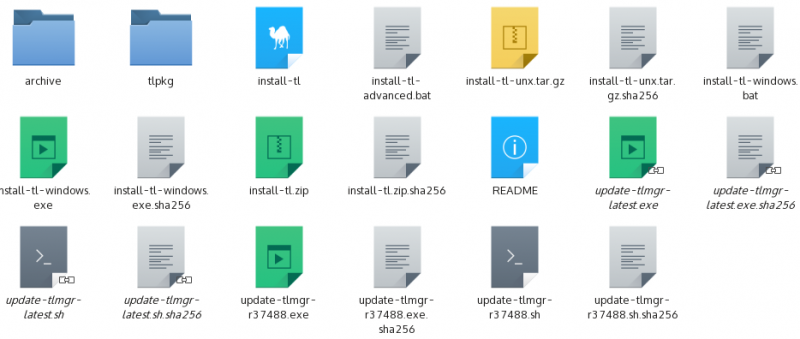
\includegraphics[width=0.65\linewidth]{Texlivefolder}
 \caption{نمایی از فایل ها و فولدرهای موجود در پوشه  \lr{TeXLive2015}}}
\end{figure}
برای مثال فرض کنید که می‌خواهیم \lr{TeXLive2015} را بر روی سیستم‌عامل ویندوز نصب کنیم. ددر روش نصب ساده شما کافی است که پنج گام زیر را طی کنید. البته قبل از آن یقیین حاصل کنید که در درایوی که می‌خواهید 
\lr{TeXLive} را نصب کنید فضای کافی وجود دارد. به عنوان نمونه برای 
\lr{TeXLive2015}
شما نیازمند حدود ۴ تا ۵ گیگ فضا هستید.
\begin{enumerate}
 \item 
 ابتدا اگر توزیع
 \lr{TeX} دیگری دارید، و یا نسخه قدیمی‌تری از 
 \lr{TeXLive}
 را دارید به طور کامل پاک کنید. گرچه نسخه‌های دیگر
 \lr{TeX} و حتی نسخه‌های گذشته 
 \lr{TeXLive} نیز می‌تواند به همراه نسخه جدید وجود داشته باشد، اما بهتر است که این‌کار انجام شود. به عنوان مثال برای پاک کردن نسخه قدیمی 
 \lr{TeXLive} به منوی \lr{Control Panel} بروید و از آن‌جا به بخش \lr{Programs and Features} بروید و \lr{TeXLive} نسخه قدیمی را پاک کنید. 
\begin{figure}[h!]
 \centering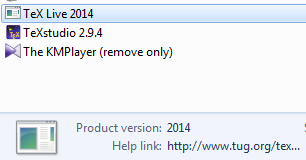
\includegraphics[scale=0.5]{UninstallTexLive}
\end{figure}
با این کار یک صفحه سیاه رنگ باز می‌شود، منتظر بمانید تا پیام \lr{Press any key} ظاهر شود، آن‌گاه می‌توانید یقین کنید که نسخه قبلی \lr{TeXLive} به صورت موفقیت آمیز پاک شده است. 
\begin{figure}[h!]
 \centering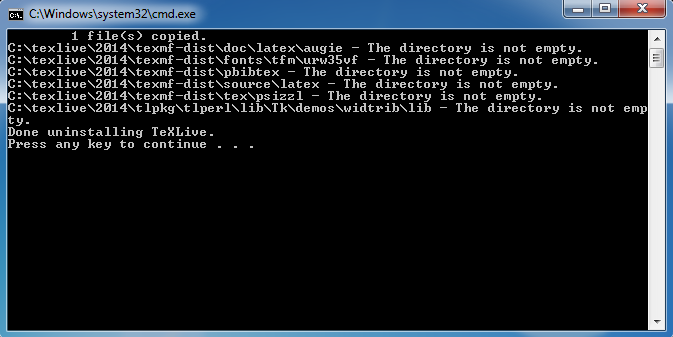
\includegraphics[scale=0.5]{Texliveuninstallcmd}
 \caption{پیام انتهایی در پایان \lr{Uninstall} برنامه \lr{TeXLive}}
\end{figure}
در ضمن می‌توانید باقیمانده فایل‌ها را نیز با مراجعه به پوشه نصب 
\lr{TeXLive} که به صورت پیش‌فرض در پوشه‌ای به نام \lr{texlive} در درایو \lr{C} قرار دارد، پاک کنید. 
\item
به پوشهٔ 
\lr{TeXLive}
بروید. روی فایل \lr{install-tl-advanced.bat} دابل کلیک کنید. (نکته: در ویندوزهای \lr{vista} به بعد باید روی فایل فوق کلیک راست کنید و \lr{Run As Administrator}
را بزنید.) 
\begin{figure}[h!]
 \centering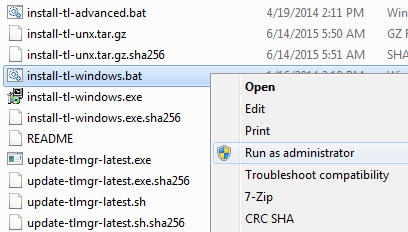
\includegraphics[scale=0.5]{InstallTexLiveRunasAdmin}
 \caption{برای نصب \lr{TeXLive} حتما گزینه \lr{Run as Administrator} را انتخاب کنید.}
\end{figure}
\item
روی \lr{Install TexLive} کلیک کنید تا نصب شروع شود. دقت کنید که در \lr{TeXLive2015} باید چندین پنجره را 
\lr{Next} بزنید تا در آخرین صفحه این دکمه را مشاهده کنید.
\begin{figure}[h!]
 \centering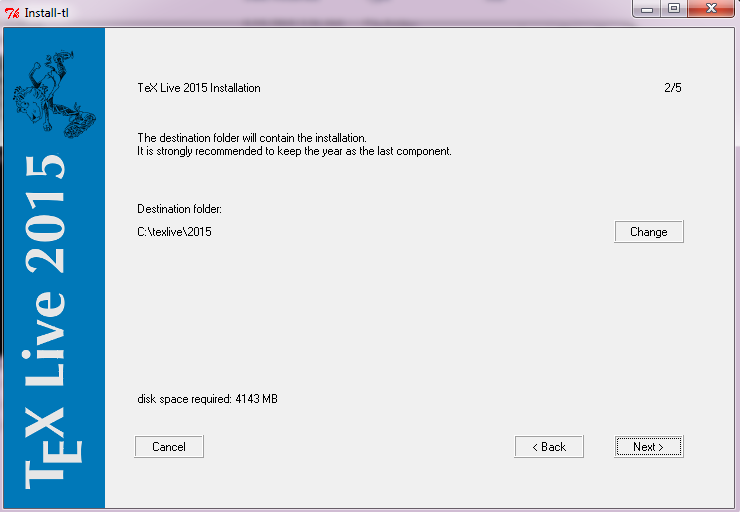
\includegraphics[scale=0.5]{InstallTexLivewindows}
 \caption{در بین صفحات نصب \lr{TeXLive2015} در یک صفحه از شما مسیری که می‌خواهید این برنامه در آن نصب شود، پرسیده می‌شود.}
\end{figure}
\item
بعد از فشردن کلید \lr{Install TexLive} پنچره‌ای به شما نشان داده می‌شود که بیانگر روند نصب بسته‌های \lr{TexLive} است. دقت کنید که به صورت همزمان یک پنجره \lr{cmd} نیز باز است که این پنجره نیز روند نصب را به شما نشان می‌دهد. صبر کنید تا هنگامی که در انتهای نصب باید پیغام \lr{Wellcome to TeX Live} را بگیرید. 
\begin{figure}[h!]
 \centering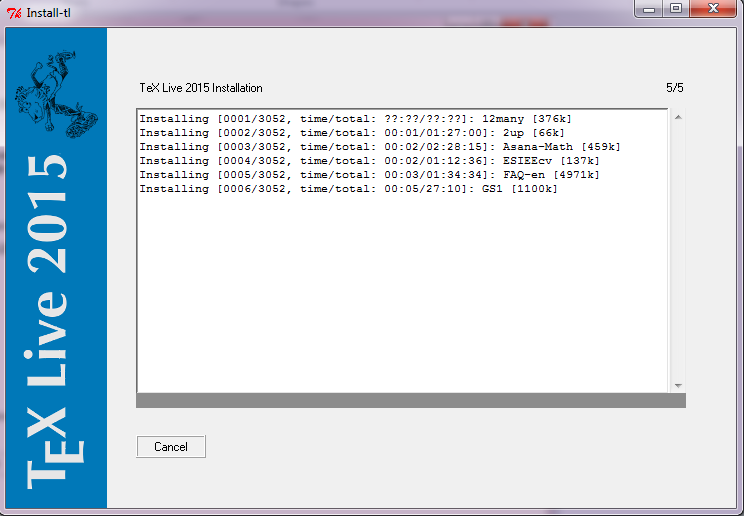
\includegraphics[scale=0.5]{InstallTexLivePackage}
 \caption{پنجره‌ای که در آن روند نصب بسته‌های \lr{LaTeX} نشان داده می‌شود.}
\end{figure}
\item
روی دکمه \lr{Finish} کلیک کنید. 
\end{enumerate}
\subsection{نصب در لینوکس}
دقت کنید که ما در این مجال دستورات را برای لینوکس \lr{Ubuntu} و \lr{Mint} آورده‌ایم. برای مابقی \lr{Linux} ها دقیقا کارهای مشابهی را باید انجام داد. 
\subsubsection{نصب به صورت \lr{command Line}}
ابتدا اگر بسته‌های تک‌لایو از قبل نصب دارید، با زدن دستور زیر در ترمینال حذف کنید.
\begin{latin}
\begin{lstlisting}[style=Mybash]‫
sudo apt-get remove texlive-*
\end{lstlisting}
\end{latin}

یک ترمینال باز کنید. به مسیر پوشه \lr{TeX Live} بروید. لیست فایل‌های موجود در پوشهٔ 
\lr{TeX Live} تقریباً باید به این صورت باشد:
\begin{latin}
\begin{lstlisting}[style=Mybash]
iran@iran:~$ cd /media
iran@iran:/media$ dir
floppy   floppy0  texlive
iran@iran:/media$ cd texlive
iran@iran:/media/texlive$ dir
archive               README
install-tl            rsync
install-tl-advanced.bat       install-tl.bat            tlpkg
install-tl-unx.tar.gz         update-tlmgr-r23180.exe
install-tl-unx.tar.gz.sha256  update-tlmgr-r23180.exe.sha256
install-tl.zip            update-tlmgr-r23180.sh
install-tl.zip.sha256         update-tlmgr-r23180.sh.sha256
\end{lstlisting}
\end{latin}
همانطور که می‌بینید فایلی با نام \lr{install-tl} هست. برای اجرای آن، دستور زیر را بزنید.
\begin{latin}
\begin{lstlisting}[style=Mybash]
sudo perl install-tl
\end{lstlisting}
\end{latin}
پیغام زیر را می‌گیرید.
\begin{latin}
\begin{lstlisting}[style=Mybash]
[sudo] password for iran:
\end{lstlisting}
\end{latin}
چون بصورت \lr{sudo} هست، پسورد کاربر جاری را از شما می‌خواهد. وارد کنید و دکمه \lr{Enter} را بزنید.

پیغام منوهای زیر ظاهر می‌شود.
\begin{latin}
\begin{lstlisting}[style=Mybash]
<O> options:‬
‪   [ ] use letter size instead of A4 by default‬
‪   [X] allow execution of restricted list of programs via \write18‬
‪   [X] create all format files‬
‪   [X] install macro/font doc tree‬
‪   [X] install macro/font source tree‬
‪   [X] after install, use tlnet on CTAN for package updates
 
‪ <V> set up for portable installation‬
 
‪Actions:‬
‪ <I> start installation to hard disk‬
‪ <H> help‬
‪ <Q> quit‬
 
‪Enter command:
\end{lstlisting}
\end{latin}
حرف
\lr{O} (اُ لاتین) را بزنید تا وارد قسمت 
\lr{Options} شوید.

حرف
\lr{L} را بزنید تا 
\lr{symlink}ها ایجاد شوند.

با این کار 
\lr{symlink}ها ایجاد می‌شوند و نیازی به اضافه کردن‌شان به 
\lr{path} سیستم نیست.

۳ تا اینتر بزنید تا مسیرهایی که پیشنهاد می‌دهد تأیید شوند. می‌توانید تغییر دهید، ولی پیشنهاد نمی‌شود.

حرف
\lr{Y} را بزنید تا بارگیری به‌روزرسانی‌های بسته‌ها بعد اتمام نصب انجام نشود. (به‌دلیل ایجاد مشکل احتمالی پیشنهاد نمی‌شود. مگر اینکه سرعت اینترنت عالی داشته باشید. پیشنهاد می‌شود بعد اتمام نصب، این کار را خودتان به جای استفاده از این گزینه، انجام دهید. یا بهتر از آن، مخزن تک‌لایو را بروزرسانی کنید و از روی آن نصب کنید.)حرف\lr{R} را بزنید که به منوی اصلی برگردید.حرف\lr{I}(آی لاتین) را زدم که نصب شروع بشه.بعد از اتمام نصب، این پیغام زیر را داد:
\begin{latin}
\begin{lstlisting}[style=Mybash]
Most importantly, add /usr/local/texlive/2011/bin/i386-linux
 to your PATH for current and future sessions.
 
 Welcome to TeX Live!
Logfile: /usr/local/texlive/2011/install-tl.log
iran@iran:/media/texlive$
\end{lstlisting}
\end{latin}
همان‌طور که می‌بینید، خطایی در مورد نصب نداده است و پیغام 
\lr{Wellcome to TeX Live} داده است.
\subsection{نصب در مکینتاش}
برای نصب تک‌لایو در مکینتاش، در
\lr{Terminal} بزنید:
\begin{latin}
\begin{lstlisting}[style=Mybash]
sudo ./install-tl.bat
\end{lstlisting}
\end{latin}
قبل شروع فرآیند نصب،
\lr{symlink} ها را در قسمت 
\lr{options} فعال کنید. یعنی بعد زدن دستور بالا، و قبل هر کاری دیگر، در پنجرهٔ ترمینال به‌ترتیب بزنید:\\
ابتدا \lr{O} سپس \lr{Y} و در آخر\lr{R} 
\section{نصب ویرایشگر}
شما می‌توانید فایل 
\lr{LaTeX} خود را در هر ویرایشگری به مانند یک 
\lr{Notepad} ساده بنویسید، و سپس با بازکردن یک 
\lr{cmd}
در ویندوز و یا
\lr{Terminal} در لینوکس، کامپایلر مورد نظر را بر روی فایل خود اجرا کنید. به عنوان مثال فایلی به نام 
\lr{sample.tex}
با محتوای زیر را در نظر بگیرید.
\begin{latin}
\begin{lstlisting}[style=Tex]
\documentclass{report}
\usepackage{xepersian}
\settextfont{XB Niloofar}
 \begin{document}
%*\rl{سلام}*)
\end{document}
\end{lstlisting}
\end{latin}
برای کامپایل این فایل کافی است که یک 
\lr{cmd}
یا
\lr{Terminal} در مسیر این فایل باز کنید و کامپایلر 
\lr{XeLaTeX} در آن تایپ کنید.
\begin{latin}
\begin{lstlisting}[style=Mybash]
xelatex sample.tex
\end{lstlisting}
\end{latin}
البته در اکثر ویرایشگرهای
\lr{LaTeX}
به مانند \lr{TeXStudio، TeXMaker} و ... امکاناتی تعبیه شده است که در همان ویرایشگر می‌توانید کامپایل مورد نظر را انجام دهید. پیش‌فرض کامپایل برخی از این ویرایشگرها \lr{pdfLaTeX} است. مسأله‌ای که وجود دارد این است که برای استفاده از بسته \lr{XePersian} می‌بایست کامپایل \lr{XeLaTeX} بر روی فایل خود انجام دهید. در این نوشتار می‌خواهیم این موضوع را مطرح کنیم که چگونه تنظیم پیش‌فرض کامپایلر این ویرایشگر‌ها را تغییر دهیم.
\subsubsection{ویرایشگر \lr{TeXStudio}}
از منوی \lr{option}، گزینه \lr{Configure TexStudio} را انتخاب کنید. از پنجره‌ای که برای شما باز می‌شود، قسمت \lr{Build} را برگزینید. در قسمت \lr{Build} از گزینه \lr{Default Compiler} کامپایلر مورد نظر خود را انتخاب کنید.
\begin{figure}[h!]
 \centering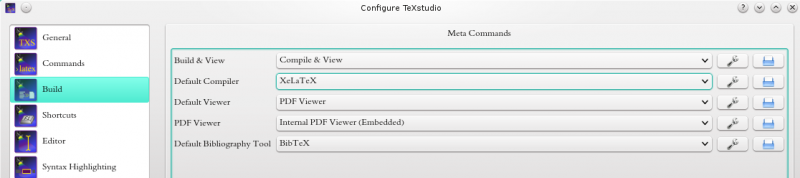
\includegraphics[scale=0.4]{Texstudioxelatex.png}
\end{figure}
البته دقت کنید که با این کار شما کامپایلر پیش‌فرض را کلا تغییر می‌دهید. اما ممکن است که شما فقط بخواهید کامپایلر پیش‌فرض بر روی \lr{XeLaTeX} باشد، اما اکنون بنا به دلیلی بخواهید دوباره \lr{pdflatex} کامپایل کنید، نیازی نیست کامپایلر پیش‌فرض را دوباره تغییر دهید. برای این‌کار از منوی \lr{Tools} قسمت \lr{Command} می‌توانید کامپایلر دلخواه خود را انتخاب کنید.
\begin{figure}[h!]
 \centering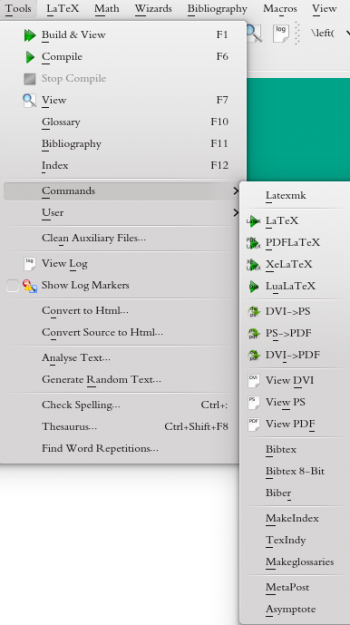
\includegraphics[scale=0.3]{Texstduianothercopmiler.png}
 \end{figure}
\subsubsection{ ویراشگر \lr{TeXmaker}}
در ویرایشگر \lr{TeXmaker} نیز از منوی \lr{option} گزینه \lr{Configure TeXmaker} را انتخاب کنید. به قسمت \lr{Quick Build} بروید. در آن‌جا می‌توانید کامپایلر مورد نظر خود را انتخاب کنید.
\begin{figure}[h!]
 \centering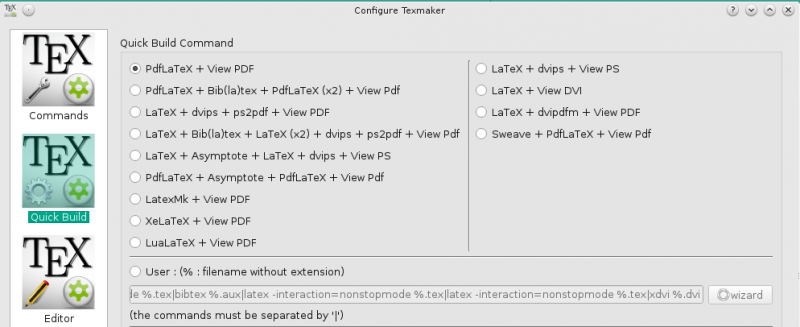
\includegraphics[width=0.80\linewidth]{TexmakerQuickbuild.png}
 \end{figure}
البته دقت کنید که با این کار شما تنظیم \lr{Quick Build} را عوض می‌کنید. در صفحه اصلی این ویرایشگر شما علاوه بر انتخاب \lr{Quick Build} می‌توانید کامپایلر مورد نظر خود را به صورت دستی نیز انتخاب کنید.
\begin{figure}[h!]
 \centering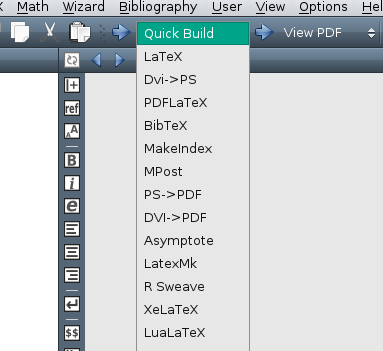
\includegraphics[scale=0.7]{Texmakermanual.png}
 \end{figure}
 
در هر ادیتوری می‌توان کدهای لاتک را نوشت اما ادیتور‌هایی هستند که به صورت گرافیکی نوشتن در محیط لاتک را آسان می‌کنند. یکی از بهترین این ادیتورها 
\lr{kile} است که می توانید از 
\href{https://kile.sourceforge.io/download.php}{https://kile.sourceforge.io/download.php}
نسخه مطلوب را برای سیستم عامل ویندوز  و یا کد منبع آن را برای سیستم عامل لینوکس دانلود کنید. همچنین با استفاده از دستور زیر در لینوکس‌ ابونتو یا مینت می‌توانید آن را نصب نمایید. تنظیمات در ان ادیتور‌ها نیز مشابه بالاست.
\begin{latin}
\begin{lstlisting}[style=Mybash]
sudo apt-get update
sudo apt-get install kile
\end{lstlisting}
\end{latin}
ادیتور‌های زیادی هستند که از لاتک برای نوشتن پشتیبانی می‌کنند منتهی برای زبان فارسی شاید مشکلاتی ایجاد کنند.
بعد از نصب \LR{TeXLive} و ادیتور می‌توانید نوشتن را شروع کنید.
\section{ساختار فایل‌های لاتک}
هر فایل لاتک از سه بخش اصلی تشکیل می‌شود. 
\begin{latin}
\begin{lstlisting}[style=Tex]
%document type
\documentclass[11pt,twoside,a4paper]{article}
%preiamble
\usepackage{xepersian}
\settextfont{XB Niloofar}
%main text
 \begin{document}
%*\rl{سلام}*)
\end{document}
\end{lstlisting}
\end{latin}
 بخش اول نوع سند را مشخص می‌کند. نوع سند می‌تواند مقاله،کتاب ، نامه و یا گزارش باشد(\lr{article, report, book, letter}). که این کلاسها به صورت پیشفرض در لاتک قرار دارند که همراه با آن نصب می شوند. برخی کلاسهای دیگر پیشفرض نیز در زیر آمده است. کلاسهای مختلفی را می‌توان در اینترنت پیدا کرد. کلاس این پایان‌نامه که iut-thesis.cls است را در پوشه آن می توانید بیابید.
   \begin{table}[h]
    \begin{latin}
  \begin{center}
 \begin{tabular}{|m{0.2\linewidth}|m{0.75\linewidth}|}
 \hline
article & For articles in scientific journals, presentations, short reports, program documentation, invitations, ...\\\hline
IEEEtran & For articles with the IEEE Transactions format.\\\hline
proc & A class for proceedings based on the article class.\\\hline
report & For longer reports containing several chapters, small books, thesis, ...\\\hline
book & For real books.\\\hline
slides & For slides. The class uses big sans serif letters.\\\hline
memoir & For changing sensibly the output of the document. It is based on the book class, but you can create any kind of document with it \\\hline
letter & For writing letters.\\\hline
beamer & For writing presentations (see LaTeX/Presentations).\\\hline
  \end{tabular}
    \end{center}
 \end{latin}
  \caption{جدول برخی کلاسهای در لاتک}
 \end{table}
 
 در همین قسمت می توان اندازه فونت پیشفرض، اندازه کاغذ و برخی ماهیت‌های سند را نیز تنظیم نمود. این ماهیت‌ها از قرار زیراند.
   \begin{table}[h!]
    \begin{latin}
  \begin{center}
 \begin{tabular}{|m{0.2\linewidth}|m{0.75\linewidth}|}
 \hline
 10pt, 11pt, 12pt &Sets the size of the main font in the document. If no option is specified, 10pt is assumed. \\\hline
a4paper, letterpaper,...&Defines the paper size. The default size is letterpaper; However, many European distributions of TeX now come pre-set for A4, not Letter, and this is also true of all distributions of pdfLaTeX. Besides that, a5paper, b5paper, executivepaper, and legalpaper can be specified. \\\hline
fleqn &Typesets displayed formulas left-aligned instead of centered. \\\hline
leqno &Places the numbering of formulas on the left hand side instead of the right. \\\hline
titlepage, notitlepage&Specifies whether a new page should be started after the document title or not. The article class does not start a new page by default, while report and book do.\\\hline
twocolumn &Instructs LaTeX to typeset the document in two columns instead of one.\\\hline
twoside, oneside&Specifies whether double or single sided output should be generated. The classes article and report are single sided and the book class is double sided by default. Note that this option concerns the style of the document only. The option twoside does not tell the printer you use that it should actually make a two-sided printout.\\\hline
landscape &Changes the layout of the document to print in landscape mode.\\\hline
openright, openany &Makes chapters begin either only on right hand pages or on the next page available. This does not work with the article class, as it does not know about chapters. The report class by default starts chapters on the next page available and the book class starts them on right hand pages.\\\hline
draft &makes LaTeX indicate hyphenation and justification problems with a small square in the right-hand margin of the problem line so they can be located quickly by a human. It also suppresses the inclusion of images and shows only a frame where they would normally occur.
\\\hline
  \end{tabular}
    \end{center}
 \end{latin}
  \caption{جدول برخی تنظیمات کلاسهای در لاتک}
 \end{table}
 
 بخش دوَم \lr{preiamble} است که محل واردکردن بسته‌های مختلف لاتک برای منظور های مختلف است. همچنین تنظیمات دیگر مربوط به بسته‌ها و یا تعریف متغییرها در این قسمت وارد می شود. از آنجایی که ما از بسته xepersian برای نوشتن فارسی استفاده می‌کنیم این بسته باید آخرین بسته‌ای باشد که فراخوانی می‌شود. هر بسته‌ای برای خود و چگونگی استفاده از آن روی اینترنت مستندات مربوط به خود را دارد.
 
 بخش سوَم مربوط به نوشتار متن و ساختار آن است. در این بخش ما از دستورات مختلف لاتک برای نوشتن سندی که می خواهیم به دست آوریم استفاده می کنیم. از فرامینی که بسته‌های لاتک در اختیار ما قرار می دهند بهره می گیریم تا به وسیله آنها فرمولها، تصاویر،زیرنویس‌ها، جداول، فصول، مراجع و... را بنویسیم. در فصل آینده دستوراتی را که در این بخش استفاده می کنیم و همچنین بسته‌های مرتبط با آنها را معرفی می‌نماییم.

\chapter{فونت و نویسه‌ها}\label{chp:chap2}
\thispagestyle{empty}
% \rhead{\leftmark}
\normalfootnotes
\section{انواع فونت‌ها در رایانه}
به یاد خالق فونت «وزیرمتن» و «فونت ساحل»  مرحوم صابر راستی کردار که فارسی نوشتن را برای فارسی نویسان عصر تکنولوژی زیبا کرد.
در حالت کلی تمامی فونت هایی که شما با آن سروکار دارید، در سه دسته کلی طبقه‌بندی می‌گردد.
\begin{description}
 \item[ فونت‌های \lr{bitmap}:] فونت‌های \lr{Bitmap} به صورت ماتریسی از نقاط بیان می‌شوند. به همین علت این فونت‌ها به سخت افزار سیستم وابسته‌ هستند و فقط در یک \lr{resolution} معین به کار می‌آیند. یک \lr{bitmap} روی صفحه ۷۵\lr{DPI} با وجود یک چاپگر ۱۲۰۰\lr{DPI} همچنان به صورت ۷۵\lr{DPI} خواهد بود. فونت‌های \lr{bitmap} صفحه نمایش معمولاً دارای پسوند \lr{bdf} یا \lr{pcf} می‌باشند. این فونت‌ها اغلب در پنجره‌ها، کنسول‌ها و ویرایشگرهای متنی کاربرد دارند، زیرا در این محلها عدم مقیاس پذیری مسئله چندان مهمی نیست.
 \item[فونت‌های \lr{Outline}:] به این دسته از فونت‌ها اصطلاحا فونت‌های برداری (\lr{vector font}) نیز گفته می‌شود. در این دسته از فونت‌ها، توصیف کلی فونت به صورت یکسری قواعد برداری و روابط ریاضیاتی بیان می‌شود، بدین‌سان این فونت‌‌ها تا هر اندازه دلخواهی توانایی مقیاس‌پذیر بودن دارند. برخی از انواع فونت های این دسته به شرح زیر است.
 \begin{latin}
\begin{itemize}
 \item Post script Type 1
    \item Post script Type 3
     \item True Type
     \item Open Type
\end{itemize}
\end{latin}
\item[فونت‌ها نوع\lr{Stroke}:] این دسته از فونت ها از یکسری خطوط به همراه توصیفی از نحوه چیدمان خطوط در کنار یکدیگر، تشکیل شده است. فونت های \lr{metafont }در این دسته جای می‌گیرند
\end{description}
\section{فونت در \lr{xepersian}}
در \lr{xepersian} شما می توانید سه دسته فونت کلی تعریف کنید. این سه دسته عبارت اند از:
\begin{itemize}
\item 
فونت مخصوص عبارات فارسی که با دستور \lr{settextfont} تعیین می شود، به عنوان مثال:
\begin{latin}
\begin{lstlisting}[style=Tex]
\settextfont{Vazirmatn}
\end{lstlisting}
\end{latin}
    فونت برای عبارات انگلیسی. اولا دقت کنید که برای این که \lr{xepersian} بتواند بفهمد که کلمه شما انگلیسی است، بدین‌سان شما باید کلمه و یا عبارت خود را درون دستور
 \lr{\textbackslash{lr}\{\}} قرار دهید، مثلا:
\begin{latin}
\begin{lstlisting}[style=Tex]
 \lr{English Words}
\end{lstlisting}
\end{latin}
و توسط دستور \lr{setlatintextfont} نیز یک فونت انگلیسی تعریف کنید. مانند آن چه که در ادامه آمده است.
\begin{latin}
\begin{lstlisting}[style=Tex]
\setlatintextfont{Vazirmatn}
\end{lstlisting}
\end{latin}
\item 
    در ضمن شما می توانید یک فونت هم برای اعداد و ارقام در فرمول های ریاضی تعریف کنید. به صورت زیر:
\begin{latin}
\begin{lstlisting}[style=Tex]
\setdigitfont{Vazirmatn}
\end{lstlisting}
\end{latin}
دقت کنید که به صورت پیش فرض اعداد و ارقام به صورت فارسی در فرمول ها در لاتک نوشته می شود، اگر بخواهد اعداد و ارقام به صورت انگلیسی در فرمول ها ظاهر شوند، کافی است دستور زیر را بنویسید:
\begin{latin}
\begin{lstlisting}[style=Tex]
\DefaultMathsDigits
\end{lstlisting}
\end{latin}
\end{itemize}
در مورد نحوه تنظیم اندازه فونت در بخش بعدی سخن به میان خواهد آمد. 
\section{اندازه فونت}
قبل از این‌که وارد بحث اصلی شویم، ابتدا باید بفهمیم که منظور از اندازه فونت چیست؟ در یک تعریف کلی به تفاوت ارتفاع بین بلندترین حرف و کوتاهترین حرف، اندازه فونت گویند.
\begin{figure}[h!]
 \centering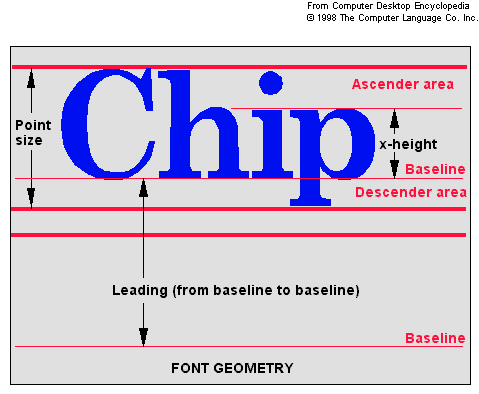
\includegraphics[scale=0.4]{8E8XO.jpg}
  \caption{تعریف اندازه فونت برای فونت های انگلیسی}
\end{figure}
اگر تاکنون با \lr{word} کار کرده اید، حتما فونت ها را با معیاری به نام اندازه می شناسید. این معیار اندازه با معیار اندازه بر حسب \lr{point} در \lr{Latex} متفاوت است. البته این تفاوت برای همه فونت ها یکسان نیست، لذا کار کمی پیچیده می شود. اما اگر در ادامه نیز همراهی کنید، فکر کنم به خوبی می توانید موضوع را متوجه شوید. فرض کنید که می‌خواهید نوشتار خود را با اندازه فونت ۱۴ در \lr{Latex} تایپ کنید. برای این کار باید چند نکته و گام را در نظر بگیرید.
\begin{figure}[h!]
 \centering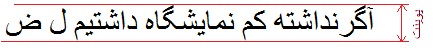
\includegraphics[scale=0.4]{FontSizePersian.jpg}
 \caption{تعریف اندازه فونت برای فونت های انگلیسی}
\end{figure}
\subsubsection{گام نخست}
در ابتدا باید یک فونت پایه برای نوشتار خود انتخاب کنید. در کل سه اندازه استاندارد برای نوشتار‌های رسمی وجود دارد:
\begin{itemize}
 \item     اندازه 10\lr{pt} که اندازه کوچک نامیده شده (که فونت‌اندازه پیشفرض تک می‌باشد.)
  \item     اندازه 11\lr{pt} که اندازه متوسط نامیده می‌شود.
   \item    اندازه 12\lr{pt} که اندازه بزرگ محصوب می‌شود.
برای تنظیم اندازه فونت پایه در lr{Latex}\ چندین روش وجود دارد، که ما در ادامه به دو مورد از آن‌ها اشاره می‌کنیم.
     \item   می توانید این مورد را در قسمت اختیاری \lr{documentclass} بنویسید. مانند:

\begin{latin}
\begin{lstlisting}[style=Tex]
\documentclass[12pt]{report}
\end{lstlisting}
\end{latin}
با این کار شما اندازه فونت پایه را 12\lr{pt} گذاشتید.

     \item   اگر دارید فایل استایل می نویسید، در دستور \lr{loadClass} عدد 12\lr{pt} را بگذارید.
\begin{latin}
\begin{lstlisting}[style=Tex]
 \LoadClass[12pt]{.....}
\end{lstlisting}
\end{latin}
     \item   در اکثر استایل‌های پیش‌فرض \lr{Latex} به مانند \lr{report، book، article، letter} و ... اندازه پیش‌فرض 10\lr{pt} است
\end{itemize}
\subsubsection{گام دوم}
اکنون شما می‌توانید با دو روش اندازه فونت خود را تعیین کنید. در روش اول، از دستور Scale در تعریف فونت استفاده می‌گردد. به عنوان مثال:
\begin{latin}
\begin{lstlisting}[style=Tex]
\settextfont[Scale=1.4]{XB Niloofar}
\setlatintextfont[Scale=1.3]{Times New Roman}
\end{lstlisting}
\end{latin}
برای مثال با اندازه فونت پایه 10\lr{pt} و Scale=1.2 اندازه فونت برابر با 12\lr{pt} خواهد شد، و یا برای اندازه فونت پایه 12\lr{pt} و \lr{Scale=1.2} اندازه فونت برابر با 14.4 خواهد شد. روش دوم مسستقل از اندازه فونت پایه است، در این روش در هرجایی از متن که می‌خواهید از دستور \lr{fontsize} به صورت زیر استفاده کنید.
\begin{latin}
\begin{lstlisting}[style=Tex]
\fontsize{x}{y}\selectfont
\end{lstlisting}
\end{latin}
در این روش از هر جایی از متن که دستورات فوق زده شود، اندازه فونت به مقدار x تنظیم خواهد شد و اندازه فاصله خط کرسی به y. البته هر جایی از متن که خواستید می‌توانید این اندازه را تغییر دهید به عنوان مثال، کد زیر را در نظر بگیرید.
\begin{latin}
\begin{lstlisting}[style=Tex]
\documentclass[10pt]{article}
\usepackage{xepersian}
\settextfont{XB Niloofar}
 
\begin{document}
%*\rl{در حالتی که اندازه‌ای تعریف نشده، نوشتار با اندازه فونت پایه چاپ می‌شود.}*)
\fontsize{13}{14}\selectfont
%*\rl{از این قسمت به بعد اندازه فونت ۱۳ خواهد شد.}*)
\fontsize{16}{17}\selectfont
%*\rl{از این قسمت به بعد اندازه فونت 16 خواهد شد.}*)
\end{document}
\end{lstlisting}
\end{latin}
خروجی در شکل زیر نشان داده شده است. 
\begin{figure}[h!]
 \centering
\includegraphics[scale=0.5]{Fontsizelatex.png}
 \caption{مثالی از تغییر اندازه فونت با دستور \lr{fontsize}}
 \end{figure}
 در کل بهتر است از روش \lr{fontsize} برای تغییر اندازه فونت به جای روش \lr{Scale} استفاده کنید. دلیلش هم این است که (۱) کیفیت در مقیاس‌های بزرگ پایین می‌آید زیرا که شما تنها ابعاد را بزرگ یا کوچک می‌کنید (۲) هیچ کنترلی روی فاصله خط کرسی وجود ندارد
\subsubsection{گام سوم}
البته قضیه بدین‌جا ختم نمی‌شود. برطبق این پست این موضوع در فونت‌های فارسی ظاهرا رعایت نمی‌شود. حروف فارسی به گونه‌ای هستند که این ارتفاع در آنها از حروف انگلیسی بیشتر است. بنابراین چنانچه ی متن فارسی با فونت ۱۲ داشته باشیم و در همان متن از فونت ۱۲ انگلیسی هم استفاده کنیم، حروف فارسی کمی کوچکتر به نظر می‌رسند. به همین دلیل در برخی از فونتها به طور عمد سایز فونت‌های فارسی را الکی بزرگ کردند تا از لحاظ ظاهری شل آنها با فونتهای انگلیسی همخوان باشد. این کار باعث به هم ریختن استاندارد شده است. در همان پست یاد شده کدهایی قرار داده شده است که شما می‌توانید نسبت دقیق را بدست آورید.
\section{فونت فارسی و انگلیسی}
در نرم افزار \lr{word} وقتی شما از یک فونت به عنوان نمونه \lr{B Nazanin} استفاده می کنید، \lr{word} در هنگام مواجه با کلمات انگلیسی، این کلمات را به یک فونت پیش فرض تبدیل می کند. چرا که اغلب فونت هایی که ما با آن ها کار می کنیم، تنها می توانند زبان فارسی و یا انگلیسی را پشتیبانی کنند. مثلا \lr{B Nazanin} فقط برای پشتیبانی از زبان فارسی است و نه برای انگلیسی. اما در \lr{LATEX} این گونه نیست. برای حل این مشکل دو راه حل دارید:
\begin{enumerate}
 \item     از فونت‌هایی استفاده کنید که هم فارسی را پشتیبانی می کنند و هم انگلیسی را، به مانند فونت‌های سری \lr{XB} مثل \lr{XB Niloofar}. برای دانلود فونت‌های از این قبیل به پیوند \lr{X Series fonts} مراجعه کنید.
  \item     در این روش، می بایست عبارات انگلیسی در متن فارسی را در داخل یک \textbackslash{lr}\{\} قرار دهید تا فهمیده شود که این عبارت باید با فونت انگلیسی نوشته شود. در این روش عبارت‌های انگلیسی با فونت انگلیسی در متن ظاهر می‌گردد.
\end{enumerate}
% نکات:
\begin{itemize}
 \item     در کل به نظر من راه حل دوم بهتر است.
  \item  در روش اوّل، نیازی نیست که کلمات انگلیسی خود را درون دستور \textbackslash{lr}\{\} قرار دهید.
\end{itemize}
\section{نحوه تعریف فونت های دیگر}
توسط دستورات 
\lr{defpersianfont} و \lr{deflatinfont} به ترتیب می توان یکسری فونت فارسی و انگلیسی دیگر تعریف کرد که در جاهای دیگر متن بتوان از آن استفاده کرد. مثلا در ادامه ما دو فونت تعریف کرده ایم:
\begin{latin}
\begin{lstlisting}[style=Tex]
\defpersianfont\myFafont[Scale=.8]{XM Traffic}
\deflatinfont\myEnfont[Scale=.9]{Adobe Arabic}
\end{lstlisting}
\end{latin}
هرگاه خواستیم یک عبارت از متن ما به صورت فونت های یادشده نوشته شود کافی است به صورت زیر عمل کنیم:
\begin{latin}
\begin{lstlisting}[style=Tex]
\myFafont{.................}
\end{lstlisting}
\end{latin}
که به جای نقطه چین کافی است عبارتی را که می خواهیم به صورت آن فونت در آید را قرار دهیم. 
\section{فونت‌های مورد نیاز قالب \lr{iut-thesis}}
تمامی فونت‌های مورد نیاز این قالب در پوشه \lr{fonts} قرارد دارد که باید آنها را نصب کنید. نصب فونت در لینوکس با قرار دادن پوشه‌ای حاوی فونت‌ها با نام \lr{.fonts} در پوشه خانگی و یک بار لاگین مجدد انجام می‌شود. در ویندوز نیز از طریق کنترل پانل و بخش فونت با کپی کردن فونت‌ها این کار صورت می پذیرد.

\chapter{نمونه‌ها و ابزار‌ها}\label{chp:chap3}
\thispagestyle{empty}
% \rhead{\leftmark}
%================================================================================
\section{مقدمه ای بر استفاده از بسته‌ها}\label{seq3.1}
در این بخش به طور خلاصه بیان می‌کنیم که چطور می‌توان شکل وارد نمود و یا نمونه کد و جدول و ... را به فایل مطلوبمان اضافه کرد. همانطور که قبلا نیز اشاره شد در لاتک با استفاده از بسته‌های مختلف می توان از ابزار‌هایی استفاده کرد که با آن اشکال، جداول، نمودارها و به طور کلی اجزای یک سند را شکل داد. این ابزارها که به صورت بسته‌های لاتک فراخوانی می‌شوند و از ابزار‌ها آنها می توان استفاده کرد. در زیر برخی از بسته‌های لاتک و امکاناتی را که در اختیار قرار می دهند آورده‌ایم.در زمان نوشتن این گفتار تعداد بسته‌های رسمی لاتک بیش از ۵۴۰۰ و بسته‌های غیر رسمی بیش از ۲۵۰۰ عدد است.
% \begin{table}
% % \begin{center}
\begin{latin}
%  \begin{tabular}{|m{0.2\linewidth}|m{0.8\linewidth}|}
\begin{longtable}{| p{.20\textwidth} | p{.80\textwidth} |}
 \hline
  amsmath &It contains the advanced math extensions for LaTeX. The complete documentation should be in your LaTeX distribution; the file is called amsdoc, and can be dvi or pdf. For more information, see the chapter about Mathematics. Successed by mathtools package described below.\\\hline
amssymb&It adds new symbols in to be used in math mode.\\\hline
amsthm&It introduces the proof environment and the {\color{green}\textbackslash{theoremstyle}} command. For more information see the Theorems section.\\\hline
array&It extends the possibility of LaTeX to handle tables, fixing some bugs and adding new features. Using it, you can create very complicated and customized tables. For more information, see the Tables section.\\\hline
babel&It provides the internationalization of LaTeX. It has to be loaded in any document, and you have to give as an option the main language you are going to use in the document. For more information see the Internationalization section.\\\hline
biblatex&Advanced bibliography handling. It is the package to use for writing a thesis.\\\hline
bm&Allows use of bold greek letters in math mode using the{\color{green} \textbackslash{bm}\{\dots\}} command. This supersedes the amsbsy package.\\\hline
booktabs &provides ex­tra com­mands as well as be­hind-the-scenes op­ti­mi­sa­tion for producing tables. Guide­lines are given as to what con­sti­tutes a good ta­ble in the package documentation.\\\hline
boxedminipage &It introduces the boxedminipage environment, that works exactly like minipage but adds a frame around it.\\\hline
caption &Allows customization of appearance and placement of captions for figures, tables, etc.\\\hline
% cancel &Provides commands for striking out mathematical expressions. The syntax is
% \begin{latin}
% \begin{lstlisting}[style=Tex]
% \cancel{x} or \cancelto{0}{x}
% \end{lstlisting}
% \end{latin}
% \\\hline
% chemmacros &Part of a bundle to typeset chemistry easily and consistent.\\\hline
% changepage &To easily change the margins of pages. The syntax is
% \begin{latin}
% \begin{lstlisting}[style=Tex]
% \changepage{textheight}{textwidth}%
%   {evensidemargin}{oddsidemargin}%
%   {columnsep}{topmargin}%
%   {headheight}{headsep}%
%   {footskip}
% \end{lstlisting}
% \end{latin}
% All the arguments can be both positive and negative numbers; they will be added (keeping the sign) to the relative variable.\\\hline
cleveref &En­hances LaTeX's cross-ref­er­enc­ing fea­tures, al­low­ing the for­mat of ref­er­ences to be de­ter­mined au­to­mat­i­cally ac­cord­ing to
the type of ref­er­ence.\\\hline
dcolumn &The package defines a new "D" column format in tab­u­lar en­vi­ron­ments for aligning the numbers in columns on the decimal point.\\\hline
enumitem &Adds support for arbitrarily-deep nested lists (useful for outlines). See List Structures.\\\hline
epstopdf &Provides and option to convert EPS images to PDF and include them with \textbackslash{includegraphics}\{\}.\\\hline
esint &Adds additional integral symbols, for integrals over squares, clockwise integrals over sets, etc.\\\hline
eucal &Other mathematical symbols.\\\hline
fancyhdr &To change header and footer of any page of the document. It is described in the Page Layout section.\\\hline
float &Im­proves the in­ter­face for defin­ing float­ing ob­jects such as fig­ures and ta­bles, introduces new floating objects types (boxed, ruled, plaintop) and provides an ability to define custom ones.\\\hline
fontenc &To choose the font encoding of the output text. You might need it if you are writing documents in a language other than English. Check in the Fonts section.\\\hline
gensymb &Pro­vides generic com­mands \textbackslash{de­gree}, \textbackslash{cel­sius}, \textbackslash{pert­hou­sand}, \textbackslash{mi­cro} and \textbackslash{ohm} which work both in text and maths mode.\\\hline
geometry &For easy management of document margins and the document page size. See Page Layout.\\\hline
glossaries &For creation of glossaries and list of acronyms. For more information, see the relevant chapter.\\\hline
graphicx &Allows you to insert graphic files within a document.\\\hline
grffile &Improves the file name pro­cess­ing of graphic/graphicx pack­ages to sup­port a larger range of file names (spaces, multiple dots, etc.).\\\hline
hyperref &It gives LaTeX the possibility to manage links within the document or to any URL when you compile in PDF. For more information, see the relevant section.\\\hline
indentfirst &Once loaded, the beginning of any chapter/section is indented by the usual paragraph indentation.\\\hline
inputenc &To choose the encoding of the input text. You might need it if you are writing documents in a language other than English. Check in the Special Characters section.\\\hline
latexsym &Other mathematical symbols.\\\hline
listings &To insert programming code within the document. Many languages are supported and the output can be customized. For more information, see the Source Code Listings.\\\hline
longtable &Al­lows you to write ta­bles that con­tinue to the next page. You can also define a header and a footer which will be shown on every page the table occupies, for example cont. from last page.\\\hline
mathptmx &Sets the default font of the entire document (including math formulae) to Times New Roman, which is a more familiar font, and useful in saving space when fighting against page limits.\\\hline
mathrsfs &Other mathematical symbols.\\\hline
mathtools &Successor of amsmath, some additional functionality, some bugs fixed.\\\hline
mhchem &allows you to easily type chemical species and equations. It automatically formats chemical species so you don't have to use subscript commands. It also Allows you to draw chemical formulas.\\\hline
microtype &It provides an improvement to LaTeX's default ty­po­graphic ex­ten­sions, improvements in such areas as char­ac­ter pro­tru­sion and font ex­pan­sion, in­ter­word spac­ing and ad­di­tional kern­ing, and hy­phen­at­able letter-spacing\\\hline
multicol &provides the mul­ti­cols environment which typesets text into multiple columns.\\\hline
natbib &Gives additional citation options and styles. Often used for journal submission.\\\hline
pdfpages &This package simplifies the insertion of external multi-page PDF or PS documents.\\\hline
rotating &It lets you rotate any kind of object. It is particularly useful for rotating tables. For more information, see the relevant section.\\\hline
setspace &Lets you change line spacing, e.g. provides the \doublespacing command for making double spaced documents. For more information, see the relevant section.\\\hline
showkeys &A useful package related to referencing. If you wish to reference an image or formula, you have to give it a name using \textbackslash{label}\{\dots\} and then you can recall it using \textbackslash{ref}\{\dots\}. When you compile the document these will be replaced only with numbers, and you can't know which label you had used unless you take a look at the source. If you have loaded the showkeys package, you will see the label just next or above the relevant number in the compiled version. An example of a reference to a section is Latex showkeys example.png. This way you can easily keep track of the labels you add or use, simply looking at the preview (both dvi or pdf). Just before the final version, remove it.\\\hline
showidx &It prints out all index entries in the left margin of the text. This is quite useful for proofreading a document and verifying the index. For more information, see the Indexing section.\\\hline
subfiles &The "root" and "child" document can be compiled at the same time without making changes to the "child" document. For more information, see the Modular Documents section.\\\hline
subcaption &It allows to define multiple floats (figures, tables) within one environment giving individual captions and labels in the form 1a, 1b.\\\hline
% syntonly &If you add the following code in your preamble:
% \begin{latin}
% \begin{lstlisting}[style=Tex]
% \usepackage{syntonly}
% \syntaxonly
% \end{lstlisting}
% \end{latin}
% LaTeX skims through your document only checking for proper syntax and usage of the commands, but doesn’t produce any (DVI or PDF) output. As LaTeX runs faster in this mode you may save yourself valuable time. If you want to get the output, you can simply comment out the second line.\\\hline
textcomp &Provides extra symbols, e.g. arrows like \textbackslash{textrightarrow}, various currencies (\textbackslash{texteuro},...), things like \textbackslash{textcelsius} and many others.\\\hline
theorem &You can change the style of newly defined theorems. For more information see the Theorems section.\\\hline
todonotes &Lets you insert notes of stuff to do with the syntax \textbackslash{todo}\{Add details.\}.\\\hline
siunitx &Helps you typeset of SI-units correctly. For example \textbackslash{SI}\{12\}\{\textbackslash{mega}\textbackslash{hertz}\}. Automatically handles the correct spacing between the number and the unit. Note that even non-SI-units are set, like dB, rad, ...\\\hline
ulem &It allows to underline text (either with straight or wavy line). Few examples of usage are added to the Fonts chapter.\\\hline
url &It defines the \textbackslash{url}\{\dots\} command. URLs often contain special character such as \'\_\' and \'\&\', in order to write them you should escape them inserting a backslash, but if you write them as an argument of \textbackslash{url}\{\dots\}, you don't need to escape any special character and it will take care of proper formatting for you. If you are using hyperref, you don't need to load url because it already provides the \textbackslash{url}\{\dots\} command.\\\hline
verbatim &It improves the verbatim environment, fixing some bugs. Moreover, it provides the comment environment, that lets you add multiple-line comments or easily comment out big parts of the code.\\\hline
xcolor &It adds support for colored text. For more information, see the relevant section.\\\hline
xypic &It is used to create trees, graphs, (commutative) diagrams, and similar things. See Xy-pic.\\\hline
% % \end{center}
\end{longtable}
%  \end{tabular}
\end{latin}
% \end{table}

\section{فرمولها}\label{seq:3.2}
فرمول‌نویسی و شماره گذاری فرمول‌ها در لاتک بسیار ساده است . کد زیر 
\begin{latin}
\begin{lstlisting}[style=Tex]
\begin{equation}\label{eq:1.2.2}
\bar{r}_{r\mathbf{R}}=\langle{\mathbf{R}n}|r|\mathbf{R}n\rangle
\end{equation}
\end{lstlisting}
\end{latin}
خروجی زیر را می دهد.
\begin{equation}\label{eq:1.2.2}
\bar{r}_{r\mathbf{R}}=\langle{\mathbf{R}n}|r|\mathbf{R}n\rangle
\end{equation}
همانطور که دیده می‌شود  برای نوشتن عبارات در فرمول‌ها از دستور زبان خاصی استفاده می شود که IDE ها معمولا این موارد را به صورت گرافیکی در اختیار قرار می دهند و افراد با استفاده از آنها به راحتی آنها را  در کد لاتک خود درج می کنند.  کلید 
\lr{\textbackslash{label\{eq:1.2.2\}}}
چاپ نمی‌شود و فقط برای ارجاع به فرمول است عبارت \lr{eq:1.2.2} یک عبارت اختیاری است که شما می توانید به دلخواه آن را تنظیم کنید و هر جایی که می‌خواهید  به فرمول فوق ارجاع دهید با استفاده از 
\lr{\textbackslash{ref\{eq:1.2.2\}}}
 می‌توانید این ارجاع را وارد کنید که در متن به شکل \ref{eq:1.2.2} چاپ می شود. مثلا می گوییم در فرمول \ref{eq:1.2.2} ما یک معادله گفتیم.
 
 فرمول‌ها می توانند چند خط باشند 
 \begin{latin}
\begin{lstlisting}[style=Tex]
 \begin{gather}
\psi _{n\mathbf{k}} ({\bf r}) = u_{n\mathbf{k}} ({\bf r})  \exp{(i\mathbf{k.r})} \\
 u_\mathbf{k}({\bf r})=u_\mathbf{k}({\bf r}+\mathbf{R})
\end{gather}
\end{lstlisting}
\end{latin}
که می شود
 \begin{gather}
\psi _{n\mathbf{k}} ({\bf r}) = u_{n\mathbf{k}} ({\bf r})  \exp{(i\mathbf{k.r})} \\
 u_\mathbf{k}({\bf r})=u_\mathbf{k}({\bf r}+\mathbf{R})
\end{gather}
ویا هم خط شده باشند
 \begin{latin}
\begin{lstlisting}[style=Tex]
\begin{align}\label{eq2}
w_n({\bf r}-\mathbf{R})=\left|\mathit{\mathbf{R}n}\right\rangle &=\frac {V}{(2\pi )^3}\int 
_{\mathit{BZ}}\mathit{d\mathbf{k}}\exp{(-\mathit{i\mathbf{k}.\mathbf{R}})}\left|\psi \right\rangle \\ 
&= \frac V{(2\pi )^3}\int 
_{\mathit{BZ}}\mathit{d\mathbf{k}}\exp{(-\mathit{i\mathbf{k}.\mathbf{R}})}u_{\mathit{n\mathbf{k}}}({\bf r})e^{\mathit{i\mathbf{k.r}}}\nonumber
\end{align}
\end{lstlisting}
\end{latin}
که می‌شود
\begin{align}\label{eq2}
w_n({\bf r}-\mathbf{R})=\left|\mathit{\mathbf{R}n}\right\rangle &=\frac {V}{(2\pi )^3}\int 
_{\mathit{BZ}}\mathit{d\mathbf{k}}\exp{(-\mathit{i\mathbf{k}.\mathbf{R}})}\left|\psi \right\rangle \\ 
&= \frac V{(2\pi )^3}\int 
_{\mathit{BZ}}\mathit{d\mathbf{k}}\exp{(-\mathit{i\mathbf{k}.\mathbf{R}})}u_{\mathit{n\mathbf{k}}}({\bf r})e^{\mathit{i\mathbf{k.r}}}\nonumber
\end{align}
که محل هم خط سازی را با علامت \lr{\&} مشخص می کنیم . گاهی نیاز است در فرمول ما شماره فرمول نداشته باشیم. برای این موارد از 
\lr{\textbackslash{nonumber}}

چنانچه بخواهیم عبارتی مانند $\epsilon$  یا  $ \bar{r}_{r\mathbf{R}}=\langle{\mathbf{R}n}|r|\mathbf{R}n\rangle$ که عباراتی ریاضی هستند در وسط متن بنویسیم آنها را  بین دو \$ قرار می دهیم. به عبارتی دیگر متن 
 \begin{latin}
\begin{lstlisting}[style=Tex]
 %*\rl{است }*) $ \bar{r}_{r\mathbf{R}}$   %*\rl{ این یک نمونه فرمول در وسط  متن }*)
\end{lstlisting}
\end{latin}
خروجی به شکل :
  این یک نمونه فرمول در وسط  متن  $ \bar{r}_{r\mathbf{R}}$ است.
  
ماتریس هم به شکل زیر نوشته می شود
 \begin{latin}
\begin{lstlisting}[style=Tex]
 \begin{equation}
  S= \begin{pmatrix}
      S_{cc} & S_{cv} \\
      S_{vc} & S_{vv}\\
      \end{pmatrix}
 \end{equation}
\end{lstlisting}
\end{latin}
که می شود
 \begin{equation}
  S=
 \begin{pmatrix}
 S_{cc} & S_{cv} \\
 S_{vc} & S_{vv}\\
 \end{pmatrix}
 \end{equation}
 
 نمونه‌ای از یک فرمول طولانی که در چند خط آمده  است به شکل زیر است.
  \begin{latin}
\begin{lstlisting}[style=Tex]
 \begin{align}
 \langle {\bf s}^{\prime}L^{\prime} | H | R{\bf s}L\rangle= & \langle {\bf s}^{\prime}L^{\prime}|-\frac{\Delta}{2} +\sum_{L_{1}} v_{{\bf s}^{\prime}L_1}(|{\bf r}-{\bf s}^{\prime}|) Y_{L_1}({\bf r}-{\bf s}^{\prime})|{\bf s}L\rangle \nonumber \\
 + & \sum_{L_{2}} v_{{\bf s}L_{2}}(|{\bf r}-R-{\bf s}) Y_{L_{2}}({\bf r}-R-{\bf s})|R{\bf s}L\rangle \nonumber \\
 + & \langle {\bf s}^{\prime}L^{\prime} | \sum_{({\bf s}^{\prime\prime}\neq)R^{\prime\prime}+{\bf s}^{\prime\prime}(\neq R+{\bf s}) , L_{1} } v_{{\bf s}^{\prime\prime}L_1}(|{\bf r}-R^{\prime\prime}-{\bf s}^{\prime\prime} |) Y_{L_{1}}({\bf r}-R^{\prime\prime}-{\bf s}^{\prime\prime}) | {\bf s}L\rangle
\end{align}
\end{lstlisting}
\end{latin}
خروجی آن نیز به شکل 
 \begin{align}
 \langle {\bf s}^{\prime}L^{\prime} | H | R{\bf s}L\rangle= & \langle {\bf s}^{\prime}L^{\prime}|-\frac{\Delta}{2} +\sum_{L_{1}} v_{{\bf s}^{\prime}L_1}(|{\bf r}-{\bf s}^{\prime}|) Y_{L_1}({\bf r}-{\bf s}^{\prime})|{\bf s}L\rangle \nonumber \\
 + & \sum_{L_{2}} v_{{\bf s}L_{2}}(|{\bf r}-R-{\bf s}) Y_{L_{2}}({\bf r}-R-{\bf s})|R{\bf s}L\rangle \nonumber \\
 + & \langle {\bf s}^{\prime}L^{\prime} | \sum_{({\bf s}^{\prime\prime}\neq)R^{\prime\prime}+{\bf s}^{\prime\prime}(\neq R+{\bf s}) , L_{1} } v_{{\bf s}^{\prime\prime}L_1}(|{\bf r}-R^{\prime\prime}-{\bf s}^{\prime\prime} |) Y_{L_{1}}({\bf r}-R^{\prime\prime}-{\bf s}^{\prime\prime}) | {\bf s}L\rangle
\end{align}
 
 می توانید در آدرس زیر فرمولها و نویسه‌های ریاضی بیشتری را ببینید. 
 \begin{latin}
\url{https://en.wikibooks.org/wiki/LaTeX/Mathematics}
\end{latin}
%%%%%%%%%%%%%%%%%%%%%%%%%%%%%%%%%%%55
\section{درج اشکال و تصاویر}\label{seq:3.3}
برای درج یک شکل در متن می‌توانیم از دستور زیر استفاده کنیم:
\begin{latin}
\begin{lstlisting}[style=Tex]
\includegraphics[scale=1]{fig-name}‎
\end{lstlisting}
\end{latin}

که در آن پارامتر اختیاری scale اندازه‌ی شکل را تعیین می‌کند و  fig-name نام شکلی است که می‌خواهیم در سند قرار دهیم. لطفا توجه فرمایید که این شکل یا باید در کنار فایل اصلی قرار داده شود و یا مانند زیر مسیر کامل آن تعریف شده باشد:
\begin{latin}
\begin{lstlisting}[style=Tex]
\includegraphics[scale=1]{/hoem/user/Desktop/fig_name}‎
\end{lstlisting}
\end{latin}
همچنین، می‌توان با استفاده از دستور زیر مسیر کلیه‌ی تصاویر را در یک پوشه تنظیم کرد:
\begin{latin}
\begin{lstlisting}
\graphicspath{ {images/} }
\end{lstlisting}
\end{latin}
که images نام پوشه‌ای است که کلیه تصاویر در آن قرار دارد.\\
توجه داشته باشید که با دستور بالا شکل مثل یک قسمت از متن تلقی می‌شود و چنانچه‌ بخواهید مکان شکل شما به صورت شناور و پویا توسط لاتک تعیین شود می‌توانید آن را در داخل یک محیط figure قرار دهید.
\begin{latin}
\begin{lstlisting}[style=Tex]
\begin{figure}[...]
\centering
\caption{%*\rl{عنوان شکل}*)}
‎\includegraphics[scale=1]{fig_name}‎
\end{figure} 
\end{lstlisting}
\end{latin}

به جای ... به عنوان پارامتر اختیاری figure می‌توانید یکی از حروف htbpH را قرار دهید یا یک رشته دلخواه از این مجموعه حروف که به ترتیب باعث می‌شوند که شکل در مکان دستور درج شکل (here)، بالای صفحه دستور درج شکل (top)، پایین صفحه دستور درج شکل (bottom)، در صفحه مجزایی شامل اجزای شناور (page of floats) و حتما در همین‌جا حتی با ناتمام گذاشتن صفحه قبل (Here) قرار گیرد.

دستور centering باعث وسط‌چین شدن شکل می‌شود، دستور caption هم باعث می‌شود که عنوان به شکل اضافه شود. توجه داشته باشید که دستور caption را می‌توانید بعد از دستور فراخوانی شکل قرار دهید تا عنوان به پایین شکل اضافه شود.

\section{مرجع‌دهی تصویر}
چنانچه مایل باشید که تصویر مورد نظر را در متن ارجاع دهید باید از label استفاده نمود. به عنوان مثال به کد زیر توجه فرمایید:
\begin{latin}
\begin{lstlisting}[style=Tex]
\begin{figure}[h]
    \centering
    \includegraphics[width=0.25\textwidth]{mesh}
    \caption{a nice plot}
    \label{fig:latex-fig}
\end{figure}
\end{lstlisting}
\end{latin}

این شکل به صورت زیر در متن ارجاع داده می‌شود:

\fcolorbox{gray!40}{gray!40}{\textcolor{black}{همانگونه که در شکل \lr{$\backslash$ref\{fig:latex-fig\}} نمایش داده شده است برای ارجاع دادن تصویر در یک متن از lable استفاده می‌شود.}}\\
نتیجه به صورت زیر مشاهده می‌شود:\\
\fcolorbox{gray!40}{gray!40}{\textcolor{black}{همانگونه که در شکل ۳ نمایش داده شده است برای ارجاع دادن تصویر در یک متن از lable استفاده می‌شود.}}
 
برای توضیحات بیشتر می توانید به لینکی که در زیر آمده است مراجعه کنید.
\begin{latin}
 \url{https://www.sharelatex.com/learn/Inserting\_Images}\\
 \url{https://en.wikibooks.org/wiki/LaTeX/Floats,_Figures_and_Captions}
\end{latin}
 
 در ادامه چند نمونه شکل آمده است که می توانید کد منبع آنها را در فایل تک پایان‌نامه ببینید. 
 
 وقتی که تنها یک شکل را بخواهیم وارد کنیم که الگوی فوق به کار می‌رود. 
 \begin{figure}[ht]
 \centering
 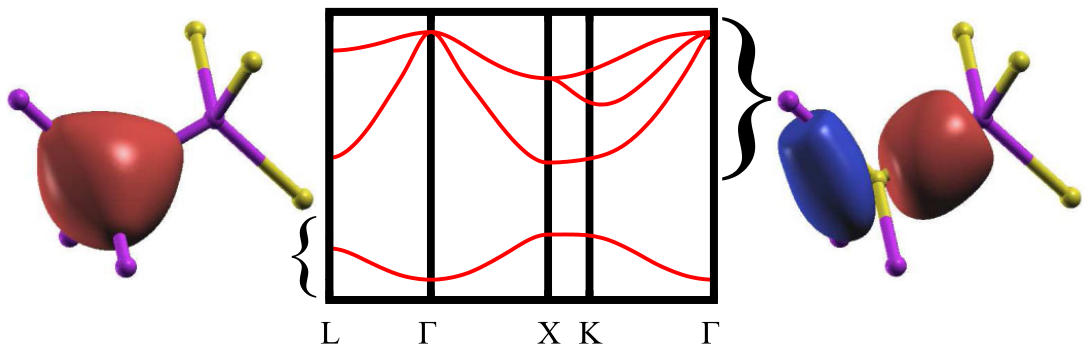
\includegraphics[scale=1.8]{GaAsps}{
\caption{\label{fig:2.2.2}
توابع وانییر بیشینه جایگزیده ساخته شده از نوار \lr{s} یا سه نوار \lr{p} در \lr{GaAs}\cite{Marzari2012}
}}
\end{figure}
 
 نمونه شکل \ref{fig:bloch} برای زمانی است که دو تصویر یا بیشتر کنار هم بخواهیم  است.
\begin{figure}[ht]
    \centering
    \begin{subfigure}[b]{0.4\textwidth}
        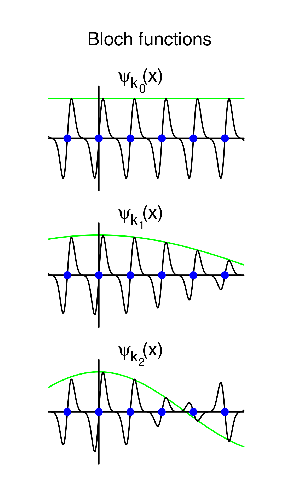
\includegraphics{bloch}
        \caption{شکل سمت راست}
        \label{fig:bloch}
    \end{subfigure}
    ~ %add desired spacing between images, e. g. ~, \quad, \qquad, \hfill etc. 
      %(or a blank line to force the subfigure onto a new line)
    \begin{subfigure}[b]{0.4\textwidth}
        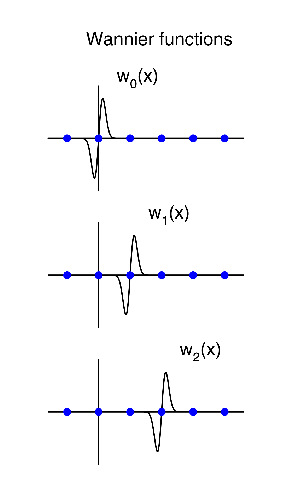
\includegraphics{wannier}
        \caption{شکل سمت چپ}
        \label{fig:wannier}
    \end{subfigure}
  \caption{
الف : توابع بلوخ متناظر با سه نقطه k مختلف در یک بعد در فضای واقعی که قسمت سبز رنگ، مربوط به پوش 
 $e^{i\mathbf{k}r}$
 است. ب : توابع وانیر جایگزیده که فضای متناظر با سمت چپ را تنیده است\cite{Marzari2012}}
\end{figure}

شکل نمونه زیر وقتی است که بخواهیم زیرنویس تصویر را کنارنویس کنیم در این صورت از بسته \lr{SCfigure} استفاده می کنیم.
\begin{SCfigure}
    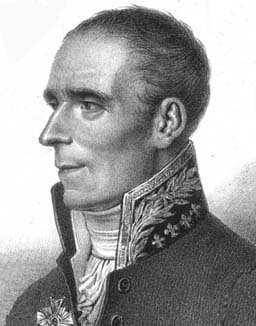
\includegraphics[width=0.35\textwidth]{Laplace}
        \caption{\protect\rule{0ex}{5ex}ایشان آقای لاپلاس است}
\end{SCfigure}
\newpage
%%%%%%%%%%%%%%%%%%%%%
\section{انواع لیست در\lr{LaTeX} }
در این بخش تلاش میگردد  انواع روش های ایجاد لیست در متن و نحوه استفاده از آنها بیان گردد. استفاده از لیست ها در 
\lr{\LaTeX}
بسیار راحت میباشد.   برای لیست هایی که نیاز به ترتیب خاص ندارند میتوان از محیط 
\lr{itemize} 
 و برای لیست های دارای ترتیب  میتوان از محیط
\lr{enumerate} 
استفاده کرد. استفاده از این دو محیط نیاز به افزودن بسته خاصی ندارد.
 برای ایجاد لیست بر اساس عنوان نیز میتوان از محیط 
\lr{decription}
استفاده کرد. لازم به ذکر است که برای استفاده از این محیط لازم است بسته
\lr{enumitem}
فراخوانی گردد.  


\subsection{لیست بدون ترتیب } 
 برای استفاده از محیط 
\lr{itemize}
 میتوان از دستور زیر استفاده نمود.
\begin{latin}
\begin{lstlisting}[style=Tex]
\begin{itemize}[label=$\ast$]
   \item %*\rl{یک}*)
   \item %*\rl{دو}*)
   \item %*\rl{سه}*)
\end{itemize}
\end{lstlisting}
\end{latin}

شایان ذکر است که آرگومان ورودی(در اینجا 
\verb![label=$\ast$]!
)
 شکل مورد استفاده برای لیست بندی را مشخص میکند.این دستور خروجی به شکل زیر ایجاد میکند.
\begin{itemize}[label=$\ast$]
\item یک
\item دو
\item سه
\end{itemize}
در صورتی که نیاز باشد نمادهای مورد استفاده در لیست تغییر کنند، میتوان بصورت زیر نمادها را تغییر داد.
\begin{latin}
\begin{lstlisting}[style=Tex]
\begin{itemize}
   \item[$-$] %*\rl{دش\hspace{2 em}}*)
   \item[$\ast$] %*\rl{ستاره}*)
   \item[$+$] %*\rl{پلاس\hspace{2 em}}*)
\end{itemize}
\end{lstlisting}
\end{latin}
که نتیجه خروجی به شکل زیر میباشد:
\begin{itemize}
    \item[$-$] دش
    \item[$\ast$] ستاره
    \item[$+$] پلاس
\end{itemize}



\subsection{لیست های دارای ترتیب }
برای ایجاد لیست دارای ترتیب میتوان از محیط 
\lr{enumerate} 
به شکل زیر استفاده نمود.
\begin{latin}
 \begin{lstlisting}[style=Tex]
\begin{enumerate}[label=\alph*)]
   \item %*\rl{یک}*)
   \item  %*\rl{دو}*)
   \item  %*\rl{سه}*)
\end{enumerate}
\end{lstlisting}
\end{latin}
 
آرگومان ورودی 
\verb![label=\alph*)]!
شیوه ترتیب بندی را مشخص میکند. میتوان از دستور 
\verb![label=(\roman*)]!
برای شماره گذاری با حروف یونانی و از دستور 
\verb![label=\arabic*)]!
برای شماره گذاری با اعداد فارسی استفاده نمود.
خروجی این دستور به شکل زیر میباشد.

\begin{enumerate}[label=\alph*)]
	\item یک
	\item دو
	\item سه
\end{enumerate}



در صورتی که در ایجاد لیست نیاز به زیرگروه نیز باشد. میتوان به شکل زیر این زیرگروهها را ایجاد کرد:


\begin{latin}
\begin{lstlisting}[style=Tex]
\begin{enumerate}[label=(\roman*)]
    \item  %*\rl{یک}*)
    \begin{enumerate}[label=(\arabic*)]
        \item  %*\rl{دو}*)
        \item  %*\rl{سه}*)
        \item  %*\rl{چهار}*)
    \end{enumerate}
    \item  %*\rl{پنج}*)
    \item  %*\rl{شش}*)
\end{enumerate}
\end{lstlisting}
\end{latin}
 که نتیجه خروجی آن به شکل زیر میباشد:

\begin{enumerate}[label=(\roman*)]
	\item یک 
    \begin{enumerate}[label=(\arabic*)]
    	\item دو
        \item سه
        \item چهار
    \end{enumerate}
    \item پنج
    \item شش
\end{enumerate}

\subsection{ایجاد لیست با عنوان دلخواه } 
برای اینکه از عناوین در ایجاد لیست استفاده شود می توان از محیط 
\lr{description}
 به صورت زیر استفاده نمود.
\begin{latin}
\begin{lstlisting}[style=Tex]
\begin{description}
   \item[Biology] %*\rl{زیست شناسی\hspace{2 em}}*) 
   \item[Physics] %*\rl{علم فیزیک\hspace{2 em}}*) 
   \item[Psychology] %*\rl{روانشناسی}*) 
\end{description}
\end{lstlisting}
\end{latin}
که نتیجه خروجی به صورت زیر میباشد:
\begin{description}
\item[Biology]  زیست شناسی
\item[Physics] علم مواد و حرکت
\item[Psychology] روانشناسی
\end{description}
%%%%%%%%%%%%%%%%%%%%5
\section{نوشتن جداول}\label{seq:3.4}
رای رسم جدول در لاتک از \lr{tabular} استفاده می‌شود. نخست باید آغاز و پایان آن را مشخص کنیم.
\begin{latin}
\begin{lstlisting}[style=Tex]
\begin{tabular}{lcr}

\end{tabular}
\end{lstlisting}
\end{latin}

هم‌زمان با این کار باید تعداد ستون‌های جدول نیز به لاتک معرفی شود. این کار با افزودن یکی از حروف c (برای ستونی با داده‌های مرکزچین)، l (برای ستونی با داده‌های چپ چین) و r (برای ستونی با داده‌های راست‌چین) داخل آکلاد انجام می‌شود، یعنی برای یک ستون راست‌چین از یک r، دو ستون راست‌چین دو r و .... سپس داده‌های سطر اول را در بین شروع و پایان محیط \lr{tabular} قرار می‌دهیم. برای رفتن به سطر بعد هم از\textbackslash\textbackslash استفاده می‌کنیم.

محیط \lr{tabular} نیز مثل یک قسمت از متن تلقی می‌شود و برای اینکه خصوصیات یک محیط پویا(شناور) را به آن بدهیم آن را در محیط \lr{table} قرار داده و از دستور مربوطه برای وسط چین کردن و دادن عنوان هم بهره خواهیم برد(همانند محیط \lr{figure} پارامترهای اختیاری مربوط به \lr{table} هم به صورت کاملا مشابه قابل تنظیم هستند).

\begin{latin}
\begin{lstlisting}[style=Tex]
\begin{table}[htbp]
\centering
\caption{title}
\begin{tabular}{lcr}
column1 & column2 & column3 \\
column1 & column2 & column3 \\
column1 & column2 & column3 \\
\end{tabular}
\end{table}
\end{lstlisting}
\end{latin}
%%%%%%%%%
\section{قالب دهی به جدول و تعریف آن به صورت شناور}

برای رسم خطوط جدا کننده در بین ستون ها یا سطرها از فرمان ها و نکات زیر استفاده می‌کنیم:
\begin{itemize}
\item  اگر به هنگام تعریف محیط \lr{tabular} در آرگومان دوم بین ستون ها از کاراکتر \textbar (پایپ) استفاده کنید، به همان ترتیب و به همان تعداد بین ستون ها خط ایجاد می‌شود.
\item برای تعریف خطوط بین سطرها باید در مکان مناسب از فرمان \lr{$\backslash$hline} استفاده کنید. به تعداد دلخواه می‌توانید از این فرمان استفاده نمایید.
\item اگر می‌خواهید در پایان جدول نیز خط افقی رسم کنید، برخلاف گفته قبلی این بار باید در انتهای سطر آخر نیز از کاراکترهای \textbackslash\textbackslash استفاده نمایید.
\item  اگر می‌خواهید به جای رسم یک خط کامل بین سطرهای جدول، از خطوط ناقص استفاده کنید، باید از فرمان زیر استفاده کنید:
\end{itemize}

\begin{latin}
\begin{lstlisting}[style=Tex]
\cline{column#1 – column#N}
\end{lstlisting}
\end{latin}

\section{تعریف جدول به صورت شناور و نحوه ارجاع دادن به آن}
برای تعریف جدول به صورت شناور و همچنین قابلیت ارجاع دهی و \lr{caption} گذاری، باید به جدول به عنوان یک موجودیت مستقل نگاه کنید. برای اینکار باید آنرا در داخل یک محیط دیگر بنام محیط \lr{table} تعریف کنید.
\begin{latin}
\begin{lstlisting}[style=Tex]
\begin{table}
\begin{tabular}
...
\end{tabular}
\end{table}
\end{lstlisting}
\end{latin}

\noindent
\textbf{
نکته ۱} : محیط \lr{table} نیز همانند محیط \lr{figure} از محیط های شناور است و خود لاتکس در مورد محل قرارگیری آن در صفحه تصمیم می‌گیرد.\\
\textbf{نکته ۲} : با استفاده از دستور

\begin{latin}
\begin{lstlisting}[style=Tex]
\caption {name}
\end{lstlisting}
\end{latin}

می‌توان به جدول زیرنویس اختصاص داد.\\
\textbf{نکته ۳: }برای ارجاع دادن به یک جدول همانند تصویر، ابتدا باید یک \lr{lable} به آن اختصاص دهید و در ادامه با استفاده از \lr{lable} به آن ارجاع دهید.

در زیر یک نمونه از جدول آمده است.
\begin{latin}
 \begin{lstlisting}[style=Tex]
 \begin{table}[ht]
\begin{center}
\caption{ %*\rl{
انتخاب‌های مختلف برای قسمت شعاعی توابع حدس اوّلیّه،}*)
$\alpha=Z/a$ \cite{Wannier902013}. \label{tab:radial2}}
\begin{latin}
\renewcommand{\arraystretch}{0.6}
\begin{tabular}{|cc|}
\hline
 $n$ & $R_{\mathrm{n}}({\bf r})$ \\\hline
1        &  $2 \alpha^{3/2}\exp(-\alpha r)$ \\\hline
2        &  $\frac{1}{2\sqrt{2}}\alpha^{3/2}(2-\alpha r)\exp(-\alpha r/2)$ \\\hline
3        &  $\sqrt{\frac{4}{27}}\alpha^{3/2}(1-2\alpha r/3+2\alpha^{2}r^{2}/27)\exp(-\alpha r/3)$ \\\hline
\end{tabular}
\end{latin}
\end{center}
\end{table}  
 \end{lstlisting}

\end{latin}
که خروجی به شکل زیر دارد
\begin{table}[ht]
\begin{center}
\caption{ 
انتخاب‌های مختلف برای قسمت شعاعی توابع حدس اوّلیّه،
$\alpha=Z/a$ \cite{Wannier902013}. \label{tab:radial2}}
\begin{latin}
\renewcommand{\arraystretch}{0.6}
\begin{tabular}{|cc|}
\hline
 $n$ & $R_{\mathrm{n}}({\bf r})$ \\\hline
1        &  $2 \alpha^{3/2}\exp(-\alpha r)$ \\\hline
2        &  $\frac{1}{2\sqrt{2}}\alpha^{3/2}(2-\alpha r)\exp(-\alpha r/2)$ \\\hline
3        &  $\sqrt{\frac{4}{27}}\alpha^{3/2}(1-2\alpha r/3+2\alpha^{2}r^{2}/27)\exp(-\alpha r/3)$ \\\hline
\end{tabular}
\end{latin}
\end{center}
\end{table}

همانطور که مشاهده می‌شود خانه‌های جدول با \& و سطور با استفاده از \textbackslash\textbackslash از هم جدا می شوند و \lr{\textbackslash{hline}} برای ایجاد خط فاصل بین سطور استفاده می‌شود. سایر ساختار در جداول مشابه به تصاویر است.
\begin{table}[h]
\begin{center}
\renewcommand{\arraystretch}{0.6}
\begin{latin}
\begin{tabular}{|c|c|c|c|}
\hline
$l$ & $m_{\mathrm{r}}$ & Name & $\Theta_{lm_{\mathrm{r}}}(\theta,\varphi)$ \\\hline
 0  &  1  &  \verb#s#   & $\frac{1}{\sqrt{4\pi}}$ \\\hline
 1  &  1  &  \verb#pz#  & $\sqrt{\frac{3}{4\pi}}\cos\theta$ \\\hline
 1  &  2  &  \verb#px#  & $\sqrt{\frac{3}{4\pi}}\sin\theta\cos\varphi$ \\\hline
 1  &  3  &  \verb#py#  & $\sqrt{\frac{3}{4\pi}}\sin\theta\sin\varphi$ \\\hline
 2  &  1  &  \verb#dz2# &$\sqrt{\frac{5}{16\pi}}(3\cos^{2}\theta -1)$ \\\hline
 2  &  2  &  \verb#dxz# & $\sqrt{\frac{15}{4\pi}}\sin\theta\cos\theta\cos\varphi$ \\\hline
 2  &  3  &  \verb#dyz# &$\sqrt{\frac{15}{4\pi}}\sin\theta\cos\theta\sin\varphi$ \\\hline
 2  &  4  &  \verb#dx2-y2# &$\sqrt{\frac{15}{16\pi}}\sin^{2}\theta\cos2\varphi$ \\\hline
 3  &  6  &  \verb#fx(x2-3y2)# & $\frac{\sqrt{35}}{4\sqrt{2\pi}}\sin^{3}\theta(\cos^{2}\varphi-3\sin^{2}\varphi)\cos\varphi$\\\hline
 3  &  7  &  \verb#fy(3x2-y2)# & $\frac{\sqrt{35}}{4\sqrt{2\pi}}\sin^{3}\theta(3\cos^{2}\varphi-\sin^{2}\varphi)\sin\varphi$\\\hline
\end{tabular}
\end{latin}
\caption{توابع زاویه‌ای}
\label{tab:angular}
\end{center}
\end{table}

نمونه زیر یک جدول فارسی است
\begin{table}[h]
\begin{center}
 \begin{tabular}
    {>{\columncolor{blue}\color{white}\bfseries}rl}
\rowcolor[gray]{0.8}
    \color{black} روز & \bfseries تعداد حاضرین\\[2pt]
دوشنبه&    57 \\  سشنبه&   11 \\
چهرشنبه& 96 \\  پنجشنبه& 122 \\
جمعه&   210 \\  شنبه& 198 \\
یکشنبه&    40 \\
\cellcolor[gray]{0.8}\color{black}جمع& 724
\end{tabular}
\caption{نمونه‌ای دیگر از جدول}
 \end{center}
\end{table}


%چنانچه بسته  float  را استفاده کنید بایستی از دستورات زیر برای تغییر در caption جداول استفاده کنید که در این صورت با فعالسازی دستور زیر از این به بعد جداول با caption  در بالا خواهند آمد. به توضیحات فایل main رجوع کنید
% \floatsetup[table]{capposition=bottom}
% \floatsetup[table]{capposition=top}

جدول به صورت لندسکیپ
 \begin{landscape}
\begin{table}[h]
\begin{center}
\caption{ انتخاب‌های مختلف برای قسمت شعاعی توابع حدس اوّلیّه،$\alpha=Z/a$ \cite{Wannier902013}. \label{tab:radial}}
\begin{latin}
\renewcommand{\arraystretch}{0.6}
\begin{tabular}{|cc|}
\hline\hline
&\\
\ \ $n$ \ \ & $R_{\mathrm{n}}({\bf r})$ \\
&\\\hline&\\
1        &  $2 \alpha^{3/2}\exp(-\alpha r)$ \\
&\\\hline&\\
2        &  $\frac{1}{2\sqrt{2}}\alpha^{3/2}(2-\alpha
r)\exp(-\alpha r/2)$ \\
&\\\hline&\\
3        &  $\sqrt{\frac{4}{27}}\alpha^{3/2}(1-2\alpha r/3+2\alpha^{2}r^{2}/27)\exp(-\alpha r/3)$ \\
&\\\hline\hline
\end{tabular}
\end{latin}
\end{center}
\end{table}
\end{landscape}
%%%%%%%%%%%%%%%%%%%%%%%%%%%%%%%%%%%%
 \section{محیط های ریاضی}
 می توانید از محیط های زیر استفاده کنید
 
 \begin{tabular}{|c|c|}
\hline
definition&section\\\hline
theorem & قضیه\\\hline
lemma&لم\\\hline
proposition&گزاره\\\hline
corollary&نتیجه\\\hline
remark&ملاحظه\\\hline
example&مثال\\\hline
\hline
 \end{tabular}
\subsection{ قضیه انتخاب}
در این قسمت نشان می دهیم
\begin{lemma}\textbf{(قطری سازی)}
نمونه یک لم اینجا آمده است.
\end{lemma}
\begin{proof}
نمونه یک اثبات  در اینجا آمده است.
\end{proof}
\begin{remark}
اگر به ازای تمام مقادیر n داشته باشیم
$|u_n(.)|\leqslant M$
\end{remark}
\begin{theorem}
نمونه ای دیگر
\end{theorem}
\begin{example}
 نمونه مثال
\end{example}
%%%%%%%%%%%%%%%%%%%%%%%
\section{\lr{tikz} و استفاده از آن}

بسته تیکز (\lr{Tikz}) احتمالاً قدرتمندترین ابزار برای تولید اشکال گرافیکی در لاتک است. به منظور استفاده از آن ابتدا باید قابلیت تصویرپردازی تیکز را با قرار دادن دستور زیر در دیباچه (\lr{preamble}) فایل متنی فعال کنید:
\begin{latin} 
\begin{lstlisting}
\usepackage{tikz}
\end{lstlisting}
\end{latin} 
محیط تصویرپردازی تیکز در متن با قرار دادن دستورات \lr{\textbackslash{begin\{tikzpicture}\}} و \lr{\textbackslash{end\{tikzpicture}\}} به ترتیب در ابتدا و انتهای دستورات این محیط فعال می‌شود. به عنوان مثال یک شکل گرافیکی را می‌توان به سادگی با تعدادی دستور مطابق زیر تولید کرد:
\begin{latin} 
\begin{lstlisting}[style=Tex]
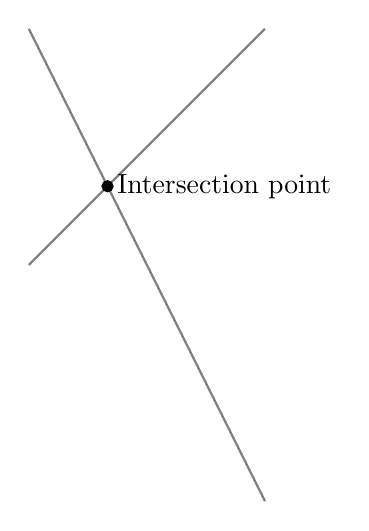
\begin{tikzpicture}
\draw[gray, thick] (-1,2) -- (2,-4);
\draw[gray, thick] (-1,-1) -- (2,2);
\filldraw[black] (0,0) circle (2pt) node[anchor=west] {Intersection point};
\end{tikzpicture}
\end{lstlisting}
\end{latin} 

خروجی این دستورات به شکل زیر است:

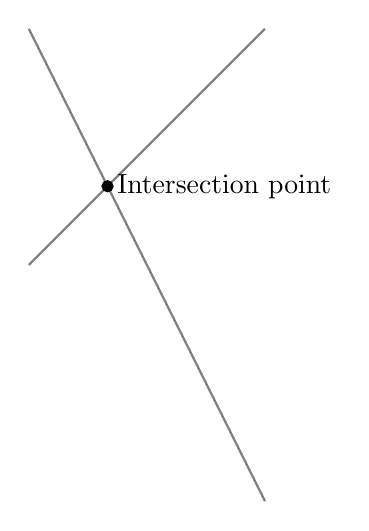
\begin{tikzpicture}
\draw[gray, thick] (-1,2) -- (2,-4);
\draw[gray, thick] (-1,-1) -- (2,2);
\filldraw[black] (0,0) circle (2pt) node[anchor=west] {Intersection point};
\end{tikzpicture}

در این مثال دو خط و یک نقطه رسم شده است. به منظور تولید خط از دستور \lr{\textbackslash{draw[gray, thick]}} استفاده شده که در آن یک المان گرافیکی تعریف شده که رنگ آن خاکستری (\lr{gray}) و ضخامت آن کلفت (\lr{thick}) است. خط در حقیقت با استفاده از دو نقطه انتهایی آن \lr{(-1,2)} و \lr{(2,-4)} که با علامت \lr{--} به هم متصل شده اند تعریف شده است. نقطه نیز در واقع یک دایره توپر است که با استفاده از دستور \lr{\textbackslash{filldraw[black]}} رسم شده است. در این دستور مرکز دایره نقطه \lr{(0,0)} و شعاع آن \lr{(2pt)} تعیین شده است. در جلوی آن یک گره (\lr{node}) تعریف شده که در حقیقت یک جعبه می‌باشد که شامل یک متن (در اینجا متن \lr{"intersection point"}) است که با دستور \lr{[anchor=west]} در سمت راست نقطه قرار داده شده است. توجه کنید که در انتهای هر دستور رسم باید علامت نقطه ویرگول (\lr{;}) را قرار دهید.

توجه: محیط رسم شکل تیکز را می‌توان در یک محیط دیگر مانند محیط شکل (\lr{figure}) قرار داد. 

شکلهای زیاد و با گرافیک بالایی را می توان با استفاده از \lr{tikz} تولید نمود .
%%%%%%%%%%%%%%%%%%%%%%%%%%%%%%%
\usetikzlibrary{lindenmayersystems}

\pgfdeclarelindenmayersystem{A}{
    \rule{F -> FF[+F][-F]}
}

\pgfdeclarelindenmayersystem{B}{
    \rule{F -> ffF[++FF][--FF]}
}

\pgfdeclarelindenmayersystem{C}{
    \symbol{G}{\pgflsystemdrawforward}
    \rule{F -> F[+F][-F]FG[+F][-F]FG}
}

\pgfdeclarelindenmayersystem{D}{
    \symbol{G}{\pgflsystemdrawforward}
    \symbol{H}{\pgflsystemdrawforward}
    \rule{F -> H[+HG][-HG]G}
    \rule{G -> HF}
}

\tikzset{
    type/.style={l-system={#1, axiom=F,order=3,step=4pt,angle=60},
      blue, opacity=0.4, line width=.5mm, line cap=round   
    },
}

\newcommand\drawsnowflake[2][scale=0.2]{
    \tikz[#1]
    \foreach \a in {0,60,...,300}  {
    \draw[rotate=\a,#2] l-system;
    };
}

\begin{center}
\foreach \width in {.2,.4,...,.8} 
{  \drawsnowflake[scale=0.3]{type=A, line width=\width mm} }

\foreach \width in {.2,.4,...,.8} 
{  \drawsnowflake[scale=0.38]{type=A, l-system={angle=90}, line width=\width mm} }    

\foreach \width in {.2,.4,...,.8} 
{  \drawsnowflake[scale=0.3]{type=B, line width=\width mm} }

\foreach \width in {.2,.4,...,.8} 
{  \drawsnowflake{type=B, l-system={angle=30}, line width=\width mm} }

\drawsnowflake[scale=0.24]{type=C, l-system={order=2}, line width=0.2mm}
\drawsnowflake[scale=0.25]{type=C, l-system={order=2}, line width=0.4mm}
\drawsnowflake[scale=0.25]{type=C, l-system={order=2,axiom=fF}, line width=0.2mm}
\drawsnowflake[scale=0.32]{type=C, l-system={order=2,axiom=---fff+++F}, line width=0.2mm}

\drawsnowflake[scale=0.38]{type=D, l-system={order=4,angle=60,axiom=GF}, line width=0.7mm}
\drawsnowflake[scale=0.38]{type=D, l-system={order=4,angle=60,axiom=GfF}, line width=0.7mm}
\drawsnowflake[scale=0.38]{type=D, l-system={order=4,angle=60,axiom=FG}, line width=0.7mm}
\drawsnowflake[scale=0.38]{type=D, l-system={order=4,angle=60,axiom=FfG}, line width=0.7mm}
\end{center}
%%%%%%%%%%%%%%%%%%%
در آدرس زیر نمونه‌های بیشتر را ببینید.
\begin{latin}
 \url{http://www.texample.net/tikz/examples/}
\end{latin}
نمونه‌ای از فلوچارت در ادامه آمده است
\begin{figure}[h!]
 \begin{center}
  \tikzstyle{startstop} = [rectangle, rounded corners, minimum width=3cm,text width=13.5em, minimum height=1cm,text badly centered, draw, fill=red!30]
  \tikzstyle{io} = [trapezium, trapezium left angle=70, trapezium right angle=110, minimum width=3cm, minimum height=1cm, text centered, draw, fill=blue!30]
  \tikzstyle{process} = [rectangle, minimum width=3cm, minimum height=1cm, text centered, draw=black, fill=orange!30]
  \tikzstyle{arrow} = [thick,->,>=stealth]
   \tikzstyle{decision} = [diamond, draw, fill=green!30,text width=4.5em, text badly centered, node distance=3cm, inner sep=0pt]
  \tikzstyle{block} = [rectangle, draw, fill=blue!20,text width=5em, text centered, rounded corners, minimum height=4em]
  \tikzstyle{line} = [draw, -latex']
  \tikzstyle{cloud} = [draw, ellipse,fill=red!20, node distance=3cm,minimum height=2em]
  \begin{tikzpicture}[node distance=2.1cm,auto]
  \node (start) [startstop] {\rl{دریافت توابع موج بلوخ از کد ساختار الکترونی و شروع فرآیند کمینه سازی}};
  \node (pro1) [process,below of=start] {$|\phi_{n\bf k}\rangle=\sum_{m}|\psi_{m\bf k}\rangle\langle\psi_{m\bf k}|g_n\rangle$};
  \node (pro2) [process,below of=pro1] {$S_{mn}^{({\bf k})}=\langle\phi_{m\bf k}|\phi_{n\bf k}\rangle=\left(A^\dagger A\right)_{mn}$};
  \node (pro3) [process,below of=pro2] {$|\tilde{\phi}_{n\bf k}\rangle=\sum_{m}\left(S^{-1/2}\right)_{mn}|\phi_{m\bf k}\rangle$};
  \node (pro4) [process,left of=start,xshift=-7cm] {$u_{n\bf k}^{(0)}({\bf k})=\exp{(-i{\bf k.r})}\tilde{\phi}_{m\bf k}({\bf r})$};
  \node (pro5) [process,below of=pro4] {$M_{mn}^{(0)({\bf k,b})}=\langle u_{m \bf k}^{(0)}|u_{m \bf k+b}^{(0)}\rangle$};
  \node (pro6) [process,below of=pro5] {$U_{mn}^{({\bf k})}=AS^{-\frac{1}{2}}$};
   \node (pro7) [process,below of=pro6] {$G^{({\bf k})}=\frac{d\Omega}{dW^{({\bf k})}}=f(M_{mn}^{\bf k,b})$};
  \node (dec1) [decision, below of=pro7] {$G^{({\bf k})}=0$};
  \node (pro8) [process,below of=dec1,yshift=-1cm] {$\Delta W^{({\bf k})}=\epsilon G^{({\bf k})}$};
  \node (pro9) [process,below of=pro8] {$U_{new}^{({\bf k})} \rightarrow U_{old}^{({\bf k})} \exp{[\Delta W^{({\bf k})}]}$};
  \node(pro10)[process,below of=pro9]{$ M^{({\bf k,b})}=U^{({\bf k})\dagger}M^{(0)({\bf k,b})}U^{({\bf k,b})}$};
  \node(result)[io,right of=dec1,xshift=6cm,yshift=-3cm]{$w_{n{\bf R}}({\bf r})=\frac{V}{(2\pi)^3}\int_{\mathrm{BZ}}\left[\sum_{m} U^{({\bf k})}_{mn} \psi_{m{\bf k}}({\bf r})\right]e^{-\mathrm{i}{\bf k}.{\bf R}} \:\mathrm{d}{\bf k}$};
  \node (end) [startstop,below of=result,yshift=-0.5cm] {\rl{پایان}};
  \draw[arrow] (start) -- (pro1);
  \draw [arrow] (pro1) -- (pro2);
  \draw [arrow] (pro2) -- (pro3);
  \draw [arrow] (pro3.west) -- node[anchor=north]{}+(-3cm,0)|-(pro4);
  \draw [arrow] (pro4)--(pro5);
  \draw [arrow] (pro5)--(pro6);
  \draw [arrow] (pro6)--(pro7);
  \draw [arrow] (pro7)--(dec1);
  \draw [arrow] (dec1.east) -- node[anchor=south]{\rl{بله}}+(7,0)-| (result);
  \draw[arrow] (dec1.south) -- node[anchor=west]{\rl{خیر}}+(0,-1)--(pro8);
  \draw[arrow] (pro8)--(pro9);
  \draw[arrow] (pro9)--(pro10);
  \draw[arrow](pro10.west)-- node[]{}+(-0.5cm,0)|-(dec1.west);
  \draw[arrow] (result)--(end);
  \end{tikzpicture}
 \end{center}
\caption{روندنمای محاسبه‌ی توابع وانییر بیشینه جایگزیده}\label{fig:3.8.1}
\end{figure}
برای دیدن چگونگی تولید روند نمای بالا با استفاده از \lr{Tikz} به کد منبع پایان‌نامه رجوع کنید.

% \chapter{مرجع فارسی}\label{chp:chap4}
\thispagestyle{empty}
%===============================
\chapter{نحوه ی تولید فایل 
	\lr{bib}
	}
	
	برای نوشتن ارجاعات در متن و تهیه‌ی لیست ارجاعات نیاز به یک فایل با پسوند 
	\lr{.bib}	
	داریم. این فایل bib‌ بعدا در انتهای متن هنگامی که دستور 
\begin{latin}
\begin{lstlisting}[style=Tex]
\bibliography{biblographyFilename.bib}
\end{lstlisting}
\end{latin}
را وارد می کنیم تا لیست مراجع را برایمان تولید کند، مورد نیاز خواهد بود.
	
	نگران دستورات نباشید در قالب همه‌ی دستورات و تنظیمات قبلا نوشته شده‌اند و شما کافی است اطلاعات خودتان را به جای اطلاعات موجود وارد کنید.
	
	برای تولید فایل با پسوند bib دو راه وجود دارد. راه اول این است که این فایل را به صورت دستی تولید کنیم. راه دوم که راه بسیار بهتری است این است که از نرم افزار های موجود که این فایل را برای ما تولید می کنند استفاده کنیم. همانند کاری که غالبا دوستان با نرم افزار EndNote در word انجام می‌دهند. من اکیدا استفاده از روش دوم یعنی استفاده از نرم افزار را پیشنهاد می‌کنم. با این حال روش دستی را نیز برای کسانی که علاقه مند هستند توضیح می‌دهم.
	\section{تولید فایل به صورت دستی }
	برای تولید فایل به صورت دستی کافی است مطابق با الگوهای زیر عمل کنید. یک فایل درست کنید و  پسوند آن را به  bib تغییر دهید . توجه داشته باشید که در هنگام نامگذاری فایل ، اسم فایل نباید دارای فاصله باشد. اطلاعات مقاله‌ی مورد نظر را با الگوی زیر وارد کنید. به جای اطلاعات داخل کروشه اطلاعات مربوط به مقاله‌ی مورد نظر را وارد کنید. برای هر مرجع یک بار باید این فرم را در همان فایل bib کپی کنید و اطلاعات آن را وارد کنید. 
\begin{latin}
	\begin{lstlisting}[style=Tex]
@article{citekey1,
	author = {Family1, Name1 and Family2, Name2},
	doi = {doiAdress},
	journal = {Jurnal Name},
	pages = {Pages},
	title = {{Article title}},
	url = {http://ulr.url},
	volume = {Volume},
	year = {1992}
	}
\end{lstlisting}
\end{latin}
در مورد کتاب می توانید به شیوه ی زیر عمل کنید.
\begin{latin}
	\begin{lstlisting}[style=Tex]
@book{citekey2,
	author = {Family1, Name1 and Family2, Name2 },
	doi = {doi},
	edition = {edition},
	editor = {Editors},
	isbn = {ISBN},
	pages = {Pages},
	publisher = {Publisher},
	title = {{Book title}}
	}
	\end{lstlisting}
\end{latin}

توجه داشته باشید که نوشتن پر کردن همه ی اطلاعات فرم های بالا ضروری نیست و اطلاعاتی را که ندارید می‌توانید پاک کنید. درآخر هم فایل را ذخیره کنید.

در مورد مراجع فارسی تنها تفاوت یک کلید اضافه است که زبان را تعیین می کند از این  رو کلید \lr{language=persian} را باید در مدخل مورد نظر وارد کنیم. نمونه‌ای از این حالت در برایتان در ادامه آورده ام.
\begin{latin}
	\begin{lstlisting}[style=Tex]
@ARTICLE{Vahedi87,
  AUTHOR =  {%*\rl{  واحدی, مصطفی} *) },
  TITLE =  {%*\rl{ درختان پوشای کمینه دورنگی مسطح}*)},
  JOURNAL =  {%*\rl{مجله فارسی نمونه}*)},
  VOLUME =  {1},
  YEAR =  {1387},
  NUMBER =  {2},
  MONTH =  {%*\rl{آبان}*)},
  PAGES =  {22-30},
  doi = {10.1103/PB.47.1651},
  language =   {Persian}
}
	\end{lstlisting}
\end{latin}
	
\section{تولید فایل به وسیله ی نرم افزار}
برای تولید این فایل نرم افزار های زیادی وجود دارد. یکی از نرم افزار‌هایی که کار را بسیار راحت کرده است نرم افزار 
\lr{Mendaley Desktop}
است. این نرم افزار  رایگان است و بر روی همه ی  سیتم عامل ها چه ویندوز ، چه لینوکس یا مک و حتی بر روی اندروید قابل نصب است. توجه داشته باشید که با هر نرم افزاری که بتوانید با آن خروجی bib بگیرید قادر هستید کارهای مراجع پایان نامه‌ی خود را انجام دهید. نرم افزار mendeley علاوه بر قابلیت‌های نرم افزار‌های دیگر، قابلیت های زیر را نیز دارد:
\begin{itemize}
	\item مدیریت فایل‌های مقالات و دسته بندی آنها را انجام می دهد.
	\item تولید فایل \lr{.bib} که مورد نیاز برای لتکس است. البته با فرمت های دیگر که برای سایر برنامه‌ها مورد نیاز است نیز فایل خروجی تولید می کند.
	\item نرم افزار اطلاعات مقاله را از فایل \lr{PDF}  به صورت هوشمند یا با استفاده از اتصال به اینترنت و از منابع مقالات نظیر \lr{Science Direct} یا \lr{Google Scholar} استخراج می کند و این یعنی در انتهای کار احتمال این که اسم نویسنده ای را اشتباه وارد کرده باشید نیست و ارجاع مقاله به فرم صحیح وارد شده است.
	\item هماهنگ سازی منابع کتابخانه ای شما در صورتی که بیش از یک دستگاه برای مطالعه دارید را انجام می‌دهد فرض کنید که چند سیستم دارید یکی در دانشکده و یکی لبتاب شخصی خودتان و شاید حتی یک سیستم در خانه، با این برنامه نیازی نیست که هر بار تمامی مقالات و یا رفرنس های خود را در بین کامپیوتر‌های خودتان منتقل کنید. هر بار که یک مقاله یا فایل را در یکی از سیستم‌هایتان وارد کردید، آن فایل بر روی تمامی سیستم‌هایتان قابل دریافت است.
	\item  امکان Highlight کردن متون و جست و جو در متن مقالات و انتخاب متن آنها یا یادداشت گذاری در مقالات به نحوی که قابل جست و جو باشد نیز وجود دارد و همه ی اینها مجددا بر روی تمامی سیستم هایی که دارید قابل مشاهده است. 
	\item پیشنهاد مقالات جدید بر اساس مقالات موجود در کتابخانه با استفاده از ایمیل. نرم افزار به صورت اتوماتیک و در صورت تمایل در موضوعاتی که مقالات آن در کتابخانه‌تان موجود است، اگر مقاله‌ی جدیدی وارد شود به شما اطلاع می‌دهد و لینک آن را برایتان ارسال می کند.
	\item  قابلیت کار با word و تولید فرمت های مورد استفاده در EndNote و \lr{JabRef}. خود نرم افزار mendeley یک افزونه دارد که در word نصب می شود و با استفاده از آن می توانید در آن محیط هم کار مراجع را سامان بدهید.
\end{itemize}

برای دانلود 
\lr{Mendaley Desktop}
کافی است  به سایتش به آدرس 
\begin{latin}
	\url{https://www.mendeley.com/}
\end{latin}
مراجعه کنید و متناسب با سیستم عاملی که در اختیار دارید نسخه ی مناسب را دانلود کنید. 

برای استفاده از قابلیت های آن کافی است یک بار  در آن ثبت‌نام کنید.
\lr{Mendaley Desktop} 
یک افزونه هم دارد که بر روی مرورگرتان نصب می شود و هر جا که مقاله ای دیدید یا حتی ویدیو با سایتی که نیاز داشته باشید به آن ارجاع بدهید، با کلیک بر روی آن اطلاعات مربوط و لازم برای ارجاع دهی را به صورت خودکار و هوشمند دریافت می کند و به کتابخانه‌تان اضافه می‌کند.
برای نصب آن به آدرس زیر در محیط برنامه بروید 
\begin{latin}
	\begin{lstlisting}[style=Tex]
Tools --> Install Web Importer
	\end{lstlisting}
\end{latin}
\section{محیط برنامه }
\begin{figure}[h]
\centering
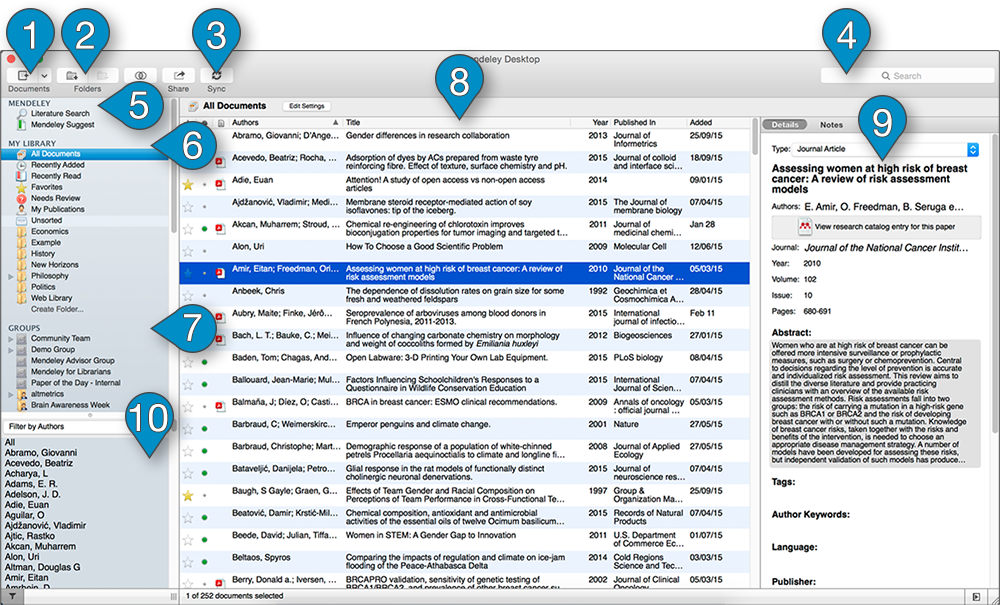
\includegraphics[width=\linewidth]{MDOverview}
\caption{شکل محیط برنامه}
\label{fig:MDOverview}
\end{figure}
به پیوست این قالب احتمالا دو فایل آموزش به صورت PDF قرار داده شده است که این نرم افزار رابه صورت کامل آموزش می‌دهند. با این حال اگر این دو فایل را نیافتید فقط کافی است به فارسی ``آموزش mendeley'' را جست و جو کنید. درضمن کتابخانه مرکزی دانشگاه هم، هر ترم دوره‌ی آموزشی این نرم‌افزار را برگزار می‌کند که خوب است شرکت کنید.
برای کسانی هم که علاقه‌مندند خودشان آموزش‌های اصلی را از سایت برنامه ببینند در آدرس زیر می‌توانند آموزش های مد نظرشان را پیدا‌کنند.
\begin{latin}
	\url{https://www.mendeley.com/guides/desktop/01-desktop-interface}
\end{latin}

فقط می ماند دو نکته که شاید به درد بخورد.

اول این که من معمولا مقاله را دانلود می کنم (به هر طریقی) بعد از آن با استفاده از 
\lr{Drag and Drop}
یا همان کشیدن و رها کردن خودمان فایل مقاله را به کتابخانه ی برنامه اضافه می کنم. حالا می‌ماند به دست آوردن مشخصات دقیق مقاله. اگر برنامه مشخصات دقیق را خودش پیدا کرده بود که هیچ، در غیر این صورت فقط کافی است 
\lr{doi}
مقاله را در قسمت 
doi
وارد کنیم و دکمه ی جست‌وجوی کنار آن را بزنیم، اطلاعات مربوط به مقاله از منابع معتبر دریافت می شود و در کتابخانه وارد می شود. 

کار وارد کردن منابع که تمام شد، آنهایی را که نیاز داریم انتخاب می کنیم. بر روی یکی از آنها کلیک راست می‌کنیم و بعد گزینه‌ی export‌ را انتخاب می‌کنیم. یک پنجره باز می شود که در آن آدرس فایل را برای ذخیره شدن انتخاب می کنیم. نام فایل را وارد می کنیم و کار تمام است. فقط حواستان باشد که نه تنها در اینجا بلکه در هیچ کجای لتکس نام هیچ فایلی را نباید با فاصله بنویسیم یعنی مثلا نباید بنویسید \lr{my biblography file name } باید همه‌ی اینها را سر‌هم بنویسید \lr{myBiblographyFileName}.

\section{نحوه‌ی ارجاع دهی در متن }
بعد از این که فایل با پسوند bib  را به هر نحوی تولید کردید نیاز است که در جاهای مختلف متن ارجاعات را مشخص کنید. اگر یادتان باشد آنجایی که داشتیم فایل bib را آماده می کردیم در ابتدای هر کدام از  ورودی ها یک عبارتی بود که من در مثال های بالا نام آنها را \lr{citekey1} و \lr{citekey2} گذاشتم. با استفاده از این کلید ها هر جای پایان نامه که باشد فرقی نمی کند (زیر عکس یا حتی در جدول ها و..) می توانید با نوشتن عبارت 
\begin{latin}
	\begin{lstlisting}[style=Tex]
\cite{citekey}
	\end{lstlisting}
\end{latin}
و آن کلید مربوطه مثلا citekey1 یا citekey2 در هر جای متن به آن مرجع به خصوص ارجاع دهید. 
در انتهای متن به صورت اتوماتیک و با تنظیمات مربوط به دانشگاه، لیست مراجع مرتب می شوند. 

\section{نحوه‌ی اجرای فایل لاتکس}
دانستن این نکته ضروری است که برای داشتن ترتیب مناسب مراجع نیاز است که لتکس را دو بار کامپایل کنید. حال اگر از برنامه های ویرایش متن خوبی نظیر texStudio استفاده می کنید، خود این برنامه‌ها این کار را برای شما اتوماتیک انجام می‌دهند و گرنه باید خودتان به این ترتیبی که می‌گویم فایل لتکس را کامپایل کنید.
\begin{enumerate}
	\item xelatex
	\item BibTex
	\item xelatex
	\item xelatex
\end{enumerate}
بار اول لتکس می فهمد که در اینجا یک سری رفرنس و مرجع وجود دارد. با اجرای مرحله‌ی دوم فایل‌های مربوط به مراجع را می‌خواند و آماده می‌کند. با اجرای مرحله ی سوم به هر مرجع در متن یک شماره می‌دهد و با اجرای مرحله‌ی چهارم این شماره‌ها را مرتب می‌کند. 
% =======================================================================
\section{ نمونه‌ هایی از مرجع زنی}\label{seq:4.1}
 در زیر نمونه‌هایی از مرجع زنی را می بینید.
 
 مرجع \cite{Vahedi87} یک نمونه مقاله مجله فارسی است.\\
مرجع \cite{Amintoosi87afzayesh}  یک نمونه  مقاله کنفرانس فارسی \\
مرجع \citep{Amintoosi87afzayesh}  یک نمونه  مقاله کنفرانس فارسی \\
نمونه ای از چند مرجع با هم \cite{Eschrig2003,Koepernik1997,Opahle1999}.
\chapter{فهرست‌ها}\label{chp:chap5}
\thispagestyle{empty}
\rhead{\leftmark}
%================================================================================
\section{فهرست مطالب ،اشکال و جداول}
وقتی شما در این پایان‌نامه و یا در کلاسهایی مثل \lr{book} برای شروع فصل از کلید 
\lr{\textbackslash{chapter}\{\}}
استفاده می کنید و یا برای بخش‌هات و زیر بخش های از 
\lr{\textbackslash{section}\{\}}
و
\lr{\textbackslash{subsection}\{\}}
سیستم لاتک خود تنطیمات ترتیب فصول را بر حسب تقدم آمدن آنها مرتب می کند. به این ترتیب هر جایی که بخواهیم فهرست مطالب چاپ شود فقط کافی است عبارت 
\lr{\textbackslash{tableofcontents}}
  اشکال و جداول نیز از قاعده‌ای مشابه پیروی می کنند و جایی که بخواهیم لیست آنها را چاپ کنیم از به ترتیب از 
  \lr{\textbackslash{listoffigures}}
  و
  \lr{\textbackslash{listoftables}}
استفاده می‌کنیم.
\section{ لغتنامه و فهرست اختصارات}\label{seq:5.2}
چگونگی اضافه کردن فهرست لغتنامه و همچنین اختصارات در آدرس زیر آمده است\\.\url{http://www.parsilatex.com/mediawiki/index.php?title=\%D8\%B1\%D8\%A7\%D9\%87\%D9\%86\%D9\%85\%D8\%A7\%DB\%8C\_\%D8\%A7\%DB\%8C\%D8\%AC\%D8\%A7\%D8\%AF\_\%D9\%88\%D8\%A7\%DA\%98\%D9\%87\%E2\%80\%8C\%D9\%86\%D8\%A7\%D9\%85\%D9\%87} \\
متن زیر چگونگی اضافه کردن و نشتن لغات و اختصارات را نشان می‌دهد.

این نمایش جایگزیده در توسعه هامیلتونی‌های مدل -هابارد، تنگابست و...- نیز به کار رفته است که موجب بررسی سیستم‌های فرمیونی هم‌بسته‌ی قوی شده است\cite{Schnell2002}. همچنین از آنها برای ساخت توابع گرین در فرمالیسم لانداور\LTRfootnote{Landauer} به منظور مطالعه رسانندگی \glspl{Ballistic}\cite{Calzolari2004}، گرمایی\cite{Paul2003} و الکتریکی\cite{Lopez-Bezanilla2009} مواد به خصوص در مواردی که سرشت کوانتومی مدنظر است، استفاده می‌شود\cite{Lee2005}.
\glspl{Quantum Transport}
زمینه‌ای است که توابع وانیر بیشینه جایگزیده در آن بسیار موفق عمل کرده است. در این شاخه به دلیل آنکه رفتار موضعی الکترون مدنظر است، این توابع با تولید ماتریس‌های هامیلتونی که بیشتر عناصر دور از قطرشان صفر است و تقریباً سه قطری هستند، امکان دستیابی به تابع گرین را راحت‌تر می‌نماید؛ از این رو در محاسبات مربوط به \glspl{Quantum Transport} بسیار سودمنداند
\cite{Kim2013}.

نمونه اختصارات میکروسکوپ\gls{AFM} و همچنین می توانید متن زیر را برای بررسی بیشتر ببینید
\\
در واقع این توابع معادل  \glspl{Localized Molecular Orbitals}هستند و تصویری از طبیعت شیمیایی پیوند‌ها در مواد ارائه می‌کنند\cite{Boys1960}. برای این منظور حالات الکترونی اشغالی را بر حسب \glspl{Maximum Localized Wannier Functions}\glsuseri{MLWFs} بسط داده و اطلاعاتی مربوط به ویژگی‌های پیوند و مختصات شیمیایی مواد را به دست می‌آورند. رفتار موضعی الکترون در برخی پدیده‌های فیزیکی مانند ترابرد کوانتومی، ناخالصی در جامدات، اتم‌های سرد و... به استفاده از نمایش جایگزیده‌ی تابع موج در فیزیک کوانتوم رونق بخشیده است. این‌گونه رفتارها در بررسی پدیده‌های الکترونیکی، اپتیک و لیزر، نانومواد و... نیز مهم هستند. در ادامه این بخش به پاره‌ای از پژوهش‌هایی که در حوزه ساختار الکترونی مواد با استفاده از توابع وانیر انجام می‌شود، به اختصار خواهیم پرداخت. برای آشنایی بیشتر با کاربردهای این توابع و به خصوص \glspl{Maximum Localized Wannier Functions}\lr{(MLWFs)} \glsuseri{MLWFs} می‌توان به مقاله‌ای که نیکولا مارزاری و دیگران در سال 2012 انتشار داده‌اند، مراجعه نمود.
 
 کد مربوط به متن فوق را می‌توانید در فایل قالب لاتک ببینید. در این پایان‌نامه و با استفاده از این متد هر جا یکی از کلمات لغتنامه و یا اختصارات آمده باشد علاوه بر ایندکس‌گذاری، کلمه مربوطه زیرنویس نیز می شود. لغتنامه اختیاری است و می توانید با کامنت کردن خط مربوط به چاپ آن در فایل \lr{main.tex}  آن را از پایان‌نامه حذف کنید.
\section{مدیریت مراجع در لاتک}\label{App:RefMan}
با دستور 
 \lr{\textbackslash bibitem}
  می‌توان یک مرجع را تعریف نمود و با فرمان
 \lr{\textbackslash cite}
  به آن ارجاع داد. این روش برای تعداد مراجع زیاد و تغییرات آنها مناسب نیست. در ادامه به صورت مختصر توضیحی در خصوص برنامه \lr{BibTeX} که همراه با توزیع‌های معروف تِک عرضه می‌شود و نحوه استفاده از آن در زی‌پرشین خواهیم داشت.

\subsection{ مدیریت مراجع با  \texorpdfstring{\lr{Bib\TeX}}{Bib\TeX} }
یکی از روش‌های قدرتمند و انعطاف‌پذیر برای نوشتن مراجع مقالات و مدیریت مراجع در لاتک، استفاده از  \lr{BibTeX} است.
 روش کار با  \lr{BibTeX} به این صورت است که مجموعه‌ی همه‌ی مراجعی را که در پروژه/پایان‌نامه/رساله استفاده کرده یا خواهیم کرد، 
در پرونده‌ی جداگانه‌ای نوشته و به آن فایل در سند خودمان به صورت مناسب لینک می‌دهیم.
 کنفرانس‌ها یا مجله‌های گوناگون برای نوشتن مراجع، قالب‌ها یا قراردادهای متفاوتی دارند که به آنها استیلهای مراجع گفته می‌شود.
 در این حالت به کمک ‌استیل‌های \lr{BibTeX} خواهید توانست تنها با تغییر یک پارامتر در پرونده‌ی ورودی خود، مراجع را مطابق قالب موردنظر تنظیم کنید. 
 بیشتر مجلات و کنفرانس‌های معتبر یک پرونده‌ی سبک (\lr{BibTeX Style}) با پسوند \lr{bst} در وب‌گاه خود می‌گذارند که برای همین منظور طراحی شده است.

به جز نوشتن مقالات این سبک‌ها کمک بسیار خوبی برای تهیه‌ی مستندات علمی همچون پایان‌نامه‌هاست که فرد می‌تواند هر قسمت از کارش را که نوشت مراجع مربوطه را به بانک مراجع خود اضافه نماید. با داشتن چنین بانکی از مراجع، وی خواهد توانست به راحتی یک یا چند ارجاع به مراجع و یا یک یا چند بخش را حذف یا اضافه ‌نماید؛ 
مراجع به صورت خودکار مرتب شده و فقط مراجع ارجاع داده شده در قسمت کتاب‌نامه خواهندآمد. قالب مراجع به صورت یکدست مطابق سبک داده شده بوده و نیازی نیست که کاربر درگیر قالب‌دهی به مراجع باشد. 
در این جا مجموعه‌ سبک‌های بسته \lr{Persian-bib} که برای  زی‌پرشین آماده شده‌اند به صورت مختصر معرفی شده و روش کار با آن‌ها گفته می‌شود. برای اطلاع بیشتر به راهنمای بسته‌ی \lr{Persian-bib} مراجعه فرمایید.
\subsection{سبک‌های فعلی قابل استفاده در زی‌پرشین}
در حال حاضر فایلهای سبک زیر برای استفاده در زی‌پرشین آماده شده‌اند:

\singlespacing
\begin{description}
\item [\lr{unsrt-fa.bst}] این سبک متناظر با \lr{unsrt.bst} می‌باشد. مراجع به ترتیب ارجاع در متن ظاهر می‌شوند.
\item [\lr{plain-fa.bst}] این سبک متناظر با \lr{plain.bst} می‌باشد. مراجع بر اساس نام‌خانوادگی نویسندگان، به ترتیب صعودی مرتب می‌شوند.
 همچنین ابتدا مراجع فارسی و سپس مراجع انگلیسی خواهند آمد.
\item [\lr{acm-fa.bst}] این سبک متناظر با \lr{acm.bst} می‌باشد. شبیه \lr{plain-fa.bst} است.  قالب مراجع کمی متفاوت است. اسامی نویسندگان انگلیسی با حروف بزرگ انگلیسی نمایش داده می‌شوند. (مراجع مرتب می‌شوند)
\item [\lr{ieeetr-fa.bst}] این سبک متناظر با \lr{ieeetr.bst} می‌باشد. (مراجع مرتب نمی‌شوند)
\item [\lr{plainnat-fa.bst}] این سبک متناظر با \lr{plainnat.bst} می‌باشد. نیاز به بسته \lr{natbib} دارد. (مراجع مرتب می‌شوند)
\item [\lr{chicago-fa.bst}] این سبک متناظر با \lr{chicago.bst} می‌باشد. نیاز به بسته \lr{natbib} دارد. (مراجع مرتب می‌شوند)
\item [\lr{asa-fa.bst}] این سبک متناظر با \lr{asa.bst} می‌باشد. نیاز به بسته \lr{natbib} دارد. (مراجع مرتب می‌شوند)
\item[\lr{ModifiedIEEEtranFa.bst}] این سبک متناظر با نحوه ارجاع در پایان‌نامه‌های دانشگاه صنعتی اصفهان می‌باشد.
\end{description}
\doublespacing

با استفاده از استیلهای فوق می‌توانید به انواع مختلفی از مراجع فارسی و لاتین ارجاع دهید. به عنوان نمونه مرجع 
\cite{Omidali82phdThesis}
 یک نمونه پروژه دکترا (به فارسی) و مرجع 
\cite{Vahedi87} یک نمونه مقاله مجله فارسی است.
مرجع 
\cite{Amintoosi87afzayesh}  یک نمونه  مقاله کنفرانس فارسی و
مرجع 
\cite{Pedram80osool} یک نمونه کتاب فارسی با ذکر مترجمان و ویراستاران فارسی است. مرجع 
\cite{Khalighi07MscThesis} یک نمونه پروژه کارشناسی ارشد انگلیسی و
\cite{Khalighi87xepersian} هم یک نمونه متفرقه  می‌باشند.
مراجع 
\cite{Gonzalez02book,Baker02limits} 
نمونه کتاب و مقاله انگلیسی هستند.

استیل مورد استفاده در این پروژه/پایان‌نامه/رساله 
\lr{ModifiedIEEEtranFa}
است که خروجی آنرا در بخش مراجع می‌توانید مشاهده کنید.
نمونه  خروجی سبک \lr{asa-fa} در شکل \ref{fig:asafa} آمده است.

\begin{figure}[t]
\centering
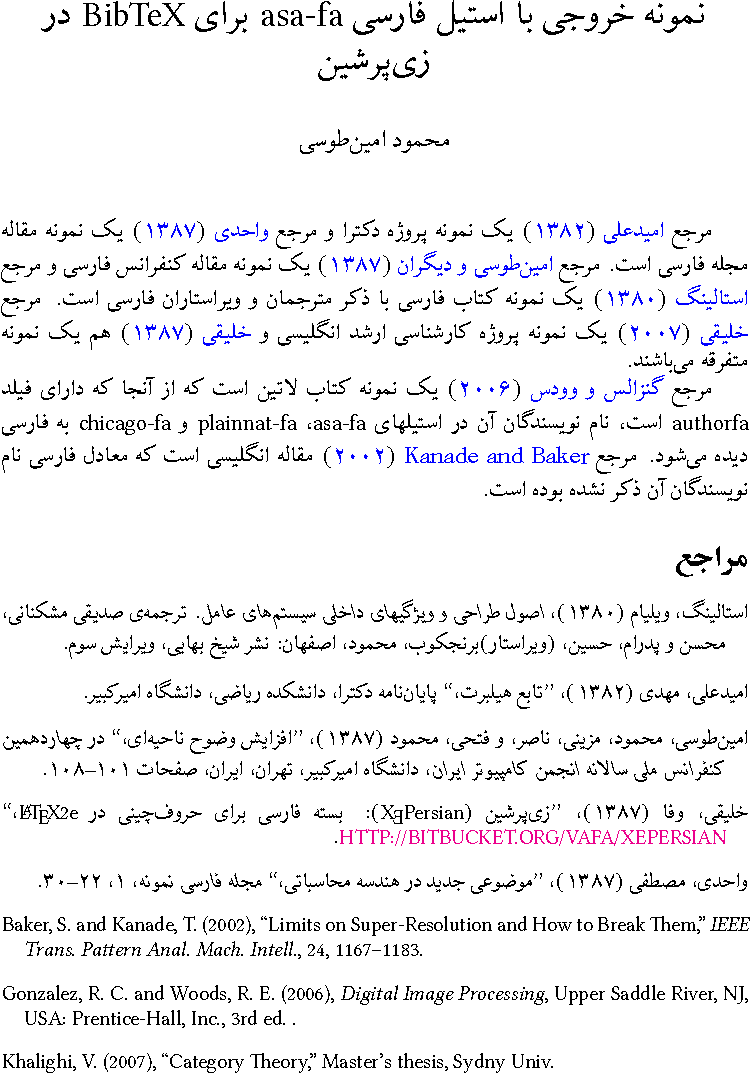
\includegraphics[width=.8\textwidth]{asa-fa-crop.pdf}
\caption{نمونه خروجی با سبک \lr{asa-fa}}
\label{fig:asafa}
\end{figure} 
\subsection{ نحوه استفاده از سبک‌های فارسی}
برای استفاده از بیب‌تک باید مراجع خود را در یک فایل با پسوند \lr{bib} ذخیره نمایید. یک فایل \lr{bib} در واقع یک پایگاه داده از مراجع\LTRfootnote{Bibliography Database}  شماست که هر مرجع در آن به عنوان یک رکورد از این پایگاه داده
با قالبی خاص ذخیره می‌شود. به هر رکورد یک مدخل\LTRfootnote{Entry} گفته می‌شود. یک نمونه مدخل برای معرفی کتاب \lr{Digital Image Processing} در ادامه آمده است:

\singlespacing
\begin{LTR}
\begin{verbatim}
@BOOK{Gonzalez02image,
  AUTHOR =      {Rafael Gonzalez and Richard Woods},
  TITLE =       {Digital Image Processing},
  PUBLISHER =   {Prentice-Hall, Inc.},
  YEAR =        {2006},
  EDITION =     {3rd},
  ADDRESS =     {Upper Saddle River, NJ, USA}
}
\end{verbatim}
\end{LTR}
\doublespacing

در مثال فوق، \lr{@BOOK} مشخصه‌ی شروع یک مدخل مربوط به یک کتاب و \lr{Gonzalez02book} برچسبی است که به این مرجع منتسب شده است.
 این برچسب بایستی یکتا باشد. برای آنکه فرد به راحتی بتواند برچسب مراجع خود را به خاطر بسپارد و حتی‌الامکان برچسب‌ها متفاوت با هم باشند معمولاً از قوانین خاصی به این منظور استفاده می‌شود. یک قانون می‌تواند فامیل نویسنده‌ی اول+دورقم سال نشر+اولین کلمه‌ی عنوان اثر باشد. به \lr{AUTHOR} و $\dots$ و \lr{ADDRESS} فیلدهای این مدخل گفته می‌شود؛ که هر یک با مقادیر مربوط به مرجع مقدار گرفته‌اند. ترتیب فیلدها مهم نیست. 

انواع متنوعی از مدخل‌ها برای اقسام مختلف مراجع همچون کتاب، مقاله‌ی کنفرانس و مقاله‌ی ژورنال وجود دارد که برخی فیلدهای آنها با هم متفاوت است. 
نام فیلدها بیانگر نوع اطلاعات آن می‌باشد. مثالهای ذکر شده در فایل \lr{References.bib} کمک خوبی به شما خواهد بود. 
%این فایل یک فایل متنی بوده و با ویرایشگرهای معمول همچون \lr{Notepad++} قابل ویرایش می‌باشد. برنامه‌هایی همچون 
%\lr{TeXMaker}
% امکاناتی برای نوشتن این مدخل‌ها دارند و به صورت خودکار فیلدهای مربوطه را در فایل \lr{bib}  شما قرار می‌دهند.  
با استفاده از سبک‌های فارسی آماده شده، محتویات هر فیلد می‌تواند به فارسی نوشته شود، ترتیب مراجع و نحوه‌ی چینش فیلدهای هر مرجع را سبک مورد استفاده  مشخص خواهد کرد.

نکته: بدون اعمال تنظیمات موردنیاز \lr{Bib\TeX} در \lr{TeXWorks}، مراجع فارسی در استیل‌هایی که مراجع را به صورت مرتب شده چاپ می‌کنند، ترتیب کاملاً درستی نخواهند داشت. برای توضیحات بیشتر \cite{persianbib87userguide} را ببینید یا به سایت پارسی‌لاتک مراجعه فرمایید.

\textbf{برای درج مراجع خود لازم نیست نگران موارد فوق باشید. در فایل 
\lr{References.bib}
 که همراه با این پروژه/پایان‌نامه/رساله هست، موارد مختلفی درج شده است و کافیست مراجع خود را جایگزین موارد مندرج در آن نمایید.
}

پس از قرار دادن مراجع خود، یک بار \lr{XeLaTeX} را روی سند خود اجرا نمایید، سپس \lr{bibtex} و پس از آن دوبار \lr{XeLaTeX} را. در \lr{TeXstudio} کلید \lr{F8} و در \lr{TeXWorks} هم گزینه‌ی \lr{BibTeX} از منوی \lr{Typeset}، \lr{BibTeX} را روی سند شما اجرا می‌کنند.

برای بسیاری از مقالات لاتین حتی لازم نیست که مدخل مربوط به آنرا خودتان بنویسید. با جستجوی نام مقاله + کلمه \lr{bibtex}  در اینترنت سایتهای بسیاری همچون \lr{ACM} و \lr{ScienceDirect} را خواهید یافت که مدخل \lr{bibtex} مربوط به مقاله شما را دارند و کافیست آنرا به انتهای فایل \lr{References} اضافه کنید.

از هر یک از سبکهای \lr{Persian-bib} می‌توانید استفاده کنید، البته اگر از سه استیل آخر استفاده می‌کنید و مایلید که مراجع شما شماره بخورند باید بسته \lr{natbib} را با گزینه \lr{numbers} فراخوانی نمایید.

%   \chapter{یک راهنما}\label{chp:chap4}
\thispagestyle{empty}
\rhead{\leftmark}
\section{نمونه لغات}
\begin{thm}\label{thm:a}
اگر $A$ و $B$ آن‌گاه $C$.
\end{thm}
در قضیه~\ref{thm:a} داریم ... \\
کلمه

برای وارد کردن یک واژه از دستور 
\lr{glspl}
باید استفاده نمود. مثل واژه 
\glspl{RandomVariable}
که اگر در فایل \lr{\TeX}  آن نگاه کنید، مشاهده می‌کنید که برای وارد کردن واژه  \glspl{RandomVariable} از دستور \lr{glspl} استفاده شده است. در ضمن  در اولین استفاده از این واژه، معادل انگلیسی آن نیز پاورقی خورده است.  و اکنون واژه \glspl{Optimization}  را تعریف می‌کنیم. 

از اختصارات، اختصارات \gls*{BAN} و \gls{CDMA} را وارد می‌کنیم. برای بار اول پاورقی می‌خورد. اما برای بار دوم پاورقی زده نمی‌شود. دقت کنید که کلمه اول یعنی چون از \lr{gls*} استفاده شده است، بار اول به حساب نمی آید. 

از اختصارات، اختصارات \gls{BAN} و \gls{CDMA} را وارد می‌کنیم. 
از اختصارات، اختصارات \gls{BAN} و \gls{CDMA} را وارد می‌کنیم. 
از اختصارات، اختصارات \gls{BAN} و \gls{CDMA} را وارد می‌کنیم. 

تا واژه و یا اختصاری را در متن با دستورات \lr{gls}‌ و \lr{glspl} وارد نکنید، واژه نه در متن ظاهر شده و نه در واژه‌نامه‌ها وارد می‌شود.
\cite{Vahedi87,Amintoosi87afzayesh}\cite{Ri2014}
استفاده از واژه‌ها و اختصارات

در بسته glossaries روش‌های مختلفی برای فراخوانی واژه‌ها و اختصارات قرار داده شده است. در ادامه به صورت مختصر این مطلب را توضیح می‌دهیم. دقت کنید که آرگومان ورودی تمامی دستورات یاد شده، label واژه و یا اختصار تعریف شده است.
gls

با این دستور معادل فارسی واژه یاد شده در مکانی که این دستور را قرار داده‌اید وارد می‌شود. مثال فرض کنید در قسمت واژه‌نامه، واژه‌ای به صورت زیر تعریف می‌کنیم.

\newword{Action}{Action}
{کنش}{کنش‌ها}

اکنون اگر در فایل tex خود می‌نویسیم.

یک ربات در مجموع تعدادی ‪\gls{Action}‬ می‌تواند انجام دهد

خروجی pdf به صورت زیر خواهد شد.

یک ربات در مجموع تعدادی کنش می‌تواند انجام دهد

در ضمن اگر این اولین باری است که از این واژه استفاده می‌کنیم، به طور خودکار معادل انگلیسی واژه استفاده شده یعنی کنش که Action است، در پاورقی وارد می‌شود.

برای اختصارات، نیز فرض کنید اختصاری به صورت زیر تعریف کرده‌ایم.

\newacronym{DFT-My}{DFT}{Discrete Fourier Transform}

اکنون در متن خود برای وارد کردن DFT می‌توانید از دستور gls استفاده کنید.

یکی از تبدیلات مهم ‪\gls{DFT-My}‬ است.

آن‌چه که شما در خروجی pdf‌ خواهید دید به صورت زیر خواهد شد.

یکی از تبدیلات مهم DFT است.

در ضمن اگر این اولین باری است که از این اختصار استفاده می‌کنیم، به طور خودکار حالت بازشده آن یعنی Discrete Fourier Transform، در پاورقی وارد می‌شود.
glspl

با استفاده از این دستور می‌توانید حالت جمع یک واژه را در متن وارد کنید. بار دیگر فرض کنید که واژه‌ای به صورت زیر در قسمت واژگان تعریف کرده‌اید.

\newword{RandomVariable}{Random Variable}
{متغیر تصادفی}{متغیرهای تصادفی}

اکنون فرض کنید که در متن فایل tex خود عبارت زیر را نوشته‌اید.

مجموع ‪\glspl{RandomVariable}‬ را می‌توان به صورت

خروجی فایل pdf چیزی شبیه به صورت زیر خواهد شد.

مجموع متغیرهای تصادفی را می‌توان به صورت

همان‌طور که مشاهده می‌کنید حالت جمع واژه RandomVariable قرار داده شده است. در ضمن اگر این کلمه برای اولین بار مورد استفاده قرار گرفته است، معادل انگلیسی حالت مقرد آن یعنی Random Variable در پاورقی وارد می‌شود.
*glspl و *gls

این دستورات به مانند glspl و gls عمل می‌کند. یعنی حالت مفرد یا جمع واژه را در متن می‌گذارد، واژه را در واژه‌نامه‌ها وارد می‌کند. اما اگر اولین مرتبه‌ای است که واژه فراخوانی می‌شود آن را پاورقی نمی‌زند. به عنوان مثال متن زیر را در نظر بگیرید.

یک ربات در مجموع تعدادی ‪\glspl*{Action}‬ می‌تواند انجام دهد. اما ‪\glspl{Action}‬ یک ربات را می‌توان

در خروجی pdf، در هر دو حالت قسمت حالت جمع واژه با برچسب Action قرار می‌گیرد. اما با این‌که در اولین جمله اولین‌باری است که کلمه Action آمده است، این کلمه پاورقی نمی‌خورد. و اولین بار فراخوانی واژه Action در جمله دوم در نظر گرفته می‌شود و همان جا نیز پاورقی ایجاد خواهد شد.

اما سوال این‌جا است که این حالت * به چه کار خواهد آمد؟ فرض کنید که شما می‌خواهید در caption یک جدول یا شکل یک واژه را بکار ببرید. مثلا فرض کنید.

\begin{figure}
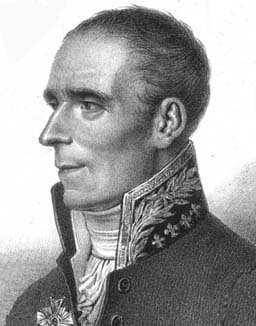
\includegraphics{Laplace.jpg}
\caption{
این مثالی از یک ‎\gls{Action}	 مجاز است.
}
\label{fig:sample1}
\end{figure}

همان‌طور که می‌دانید caption ها اشکال در فهرست اشکال جمع‌آوری می‌شوند، و به احتمال زیاد اولین جایی که واژه Action بکار می‌رود در caption ها است که در فهرست اشکال آورده شده است. پرواضح است که ما نمی‌خواهیم در فهرست اشکال پاورقی داشته باشیم. پس بهتر است که در caption‌ جداول و اشکال از حالت * دستورات استفاده کنیم. یعنی:

\begin{figure}
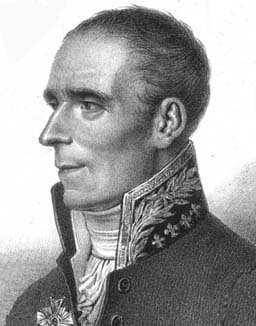
\includegraphics{Laplace.jpg}
\caption{
این مثالی از یک ‪‎\gls*{Action}‬ مجاز است.
}
\label{fig:sample4}
\end{figure}

glsentrytext

این دستور به مانند gls است. با این تفاوت که فقط در متن قسمت text اختصار یا واژه مورد نظر وارد می‌شود، و واژه مورد نظر نه پاورقی می‌خورد و نه در واژه‌نامه‌ها وارد می‌شود. برای واژه و اختصار زیر را در نظر بگیرید.

\newword{Optimization}{Optimization}{بهینه‌سازی}{}
 
\newacronym{DFT}{DFT}{Discrete Fourier Transform}

اکنون اگر در متن خود بنویسید:

می‌توانیم با ‎\glsentrytext{Optimization}‎ تبدیل ‎\glsentrytext{DFT}‎ را

شما در خروجی pdf عبارت زیر را مشاهده خواهید کرد.

می‌توانیم با بهینه‌سازی تبدیل DFT را


اماواژه Optimization و اختصار DFT اگر در این جا حتی اولین باری باشد که بکار رفته باشد، دیگر پاورقی نخواهد خورد، در ضمن این واژه و اختصار وارد واژه‌نامه و فهرست اختصارات نیز نخواهد شد.
glsentryplural

این دستور به مانند glspl است. با این تفاوت که فقط در متن قسمت جمع واژه مورد نظر وارد می‌شود، و واژه مورد نظر نه پاورقی می‌خورد و نه در واژه‌نامه‌ها وارد می‌شود.
glsuseri

اگر از این دستور استفاده کنید، واژه و یا اختصار در متن نمی آید اما در واژه نامه و یا فهرست اختصارات وارد می‌شود. 

\begin{figure}[ht]
\centering
\fbox{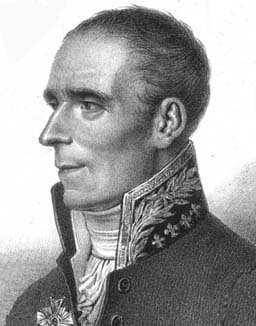
\includegraphics[scale=.5]{Laplace.jpg}}
%\captionsetup{textfont=rm,justification=centering,labelsep=newline}
\caption{\label{fig:laplace} پیر سیمون لاپلاس}
\end{figure}
%\end{document}

  

%با تکرار و اضافه کردن خطوط فوق می توانید فصل اضافه کنید .فایلهای تک درون فولد chapter فایلهای مربوط به هر کدام از فصل هاست.به ساختار آنها و labelها دقت کنید.
%===================================== Print Bibs & Glossaries
% خطوط زیر برای اضافه نمودن و تفکیک فصول پیوست است
\appendix
 % !TEX TS-program = XeLaTeX
% !TeX root=main.tex
% دستورات زیر باید در اولین فایل پیوست باشند. آنها را حذف نکنید!    
\chapter{نمونه‌هایی برای وارد کردن کد برنامه‌ها}\label{App:RefMan1}
\thispagestyle{empty}
%==================================================================
نمونه کد \lr{C}
\begin{latin}
\begin{lstlisting}[style=CStyle]
#include <stdio.h>
int main(void)
{
   printf("Hello World!"); 
}
\end{lstlisting}
\end{latin}
نمونه کد بش:
\begin{latin}
\begin{lstlisting}[style=Mybash]
 ~$ sudo apt-get update & sudo apt-get upgrade
 ~$ sudo apt-get install python3 python3-numpy python3-scipy
 ~$ chmod +x fplo2wannier
\end{lstlisting}
\end{latin}
نمونه کد پایتون:
\begin{latin}
\begin{lstlisting}[style=Mypython]
 #!/usr/bin/python3 -u
from sys import argv
arg=[int(x) for x in argv[1:4]]
xtel=1.0/arg[0]
ytel=1.0/arg[1]
ztel=1.0/arg[2]
x,y,z=0.0,0.0,0.0
with open("./wankp","w") as f:
	f.write("%s f 1 1 \n"%(arg[0]*arg[1]*arg[2]))
	
for z in range(arg[2]):
	for y in range(arg[1]):
		for x in range(arg[0]):
			with open("./=.kp","a") as f:
				f.write("%s %s %s\n"%(repr(x*xtel).ljust(20),
                repr(y*ytel).ljust(20),repr(z*ztel).ljust(20)))
				print("%s %s %s\n"%(repr(x*xtel).ljust(20),
                repr(y*ytel).ljust(20),repr(z*ztel).ljust(20)))
\end{lstlisting}
\end{latin}
% \end{landscape}
نمونه کد برای زبان جولیا
\begin{latin}
\begin{lstlisting}[style=julia]
#= This is a code sample for the Julia language
(adapted from http://julialang.org) =#
function mandel(z)
    c = z
    maxiter = 80
    for n = 1:maxiter
        if abs(z) > 2
            return n-1
        end
        z = z^2 + c
    end
    return maxiter
end

function helloworld()
    println("Hello, World!") # Bye bye, MATLAB!
end

function randmatstat(t)
    n = 5
    v = zeros(t)
    w = zeros(t)
    for i = 1:t
        a = randn(n,n)
        b = randn(n,n)
        c = randn(n,n)
        d = randn(n,n)
        P = [a b c d]
        Q = [a b; c d]
        v[i] = trace((P.'*P)^4)
        w[i] = trace((Q.'*Q)^4)
    end
    std(v)/mean(v), std(w)/mean(w)
end
\end{lstlisting}
\end{latin}
نمونه کد برای کد متلب
\begin{latin}
 \begin{lstlisting}[style=mymatlab]
  n = 40;
y = randi([500, 600], 1, n);
a = zeros(n,1);

% PARFOR-Loop (no workers)
if matlabpool('size') > 0, matlabpool close, end

p1 = Par(n);

parfor id = 1:n
  Par.tic;
  a(id) = max(svd(rand(y(id))));
  p1(id) = Par.toc;
end

stop(p1);

plot(p1);

% Plot using optional colormap input
% plot(p1,@bone);
 \end{lstlisting}
\end{latin}
نمونه کد برای فرترن
\begin{latin}
 \begin{lstlisting}[style=myfortran]
! Der folgende Fortran-Code ist bei Wikipedia geklaut.
SUBROUTINE test( Argument1, Argument2, Argument3 )
   REAL,              INTENT(IN) :: Argument1
   CHARACTER(LEN= *), INTENT(IN) :: Argument2
   INTEGER,           INTENT(IN), OPTIONAL :: Argument3
   ! This makes sense
END SUBROUTINE
\end{lstlisting}
\end{latin}



%  \chapter{راهنمای محیط پردازش تصویر \lr{Tikz}}\label{appen2}
\thispagestyle{empty}
% \chapter{مدیریت مراجع درتک}\label{App:Refan}
\thispagestyle{empty}
\chapter{اتصال بسته محاسباتی \lr{FPLO} و\lr{Wannier90}}\label{chp:chap4}
\thispagestyle{empty}
\rhead{\leftmark}
%================================================================================

\section{چگالی‌ حالات هیبریدی و هیبریدی منطقه ای }\label{seq:4.2}
چگالی حالات کل الکترون‌ها در یک ساختار از عبارت زیر حاصل می‌شود:\cite{Martin2004}
\begin{equation}
 \rho(\varepsilon)=\frac{1}{N_{{\bf k}}}\sum_{n,{\bf k}}\delta(\varepsilon_{n,{\bf k}}-\varepsilon)=\frac{V_{cell}}{(2\pi)^d} \int_{BZ} d{\bf k}\delta(\varepsilon_{n,{\bf k}}-\varepsilon)
\end{equation}
که با نوشتار دیراک 
\begin{equation}
 \rho(\varepsilon)=\sum_{n}\langle\psi_n|\psi_n\rangle\delta(\varepsilon_{n}-\varepsilon)
\end{equation}
هم ارز است  و در آن $\varepsilon_n$ ویژه مقدار ویژه حالت $\psi_n$ است. با استفاده از پایه‌های کامل و بهنجار $|i\rangle\langle i|=1$ و $|r\rangle\langle r|=1$ می‌توانیم عبارات زیر را بنویسیم.
\begin{align}
\rho_{i}(\varepsilon)=\sum_n\langle\psi_n|i\rangle\langle i|\psi_n\rangle\delta(\varepsilon-\varepsilon_n)\label{eq:4.2.3}\\
\rho(r,\varepsilon)=\sum_n\langle\psi_n|r\rangle\langle r|\psi_n\rangle\delta(\varepsilon-\varepsilon_n)\label{eq:4.2.4}
\end{align}
عبارات فوق به ترتیب \glspl{چگالی حالات تصویر شده}و \glspl{چگالی حالات موضعی}هستند.\cite{gpaw} 
اربیتال‌های $|i\rangle$ و $|r\rangle$ می‌توانند هر اربیتال دلخواه انتخابی- با رعایت شرط کاملیّت و بهنجار 
بودن- باشند؛ امّا ما در محاسبات خود در برنامه \lr{FPLO2WANNIER} از بخش زاویه‌ای توابع $g_n$ که در 
بخش \ref{seq:4.1} معرفی شده‌اند یعنی $\Theta_{lm_{\mathrm{r}}}(\theta,\varphi)$های معرفی شده در جداول 
\ref{tab:angular} و \ref{tab:hybrids} به عنوان توابع انتخابی استفاده نموده‌ایم. لازم به یادآوری است که 
جدول \ref{tab:angular} اربیتالهای اتمی و جدول  \ref{tab:hybrids} اربیتال‌های هیبریدی را به دست می‌دهد و 
تنها بخش حقیقی آنها را شامل می‌شود؛\cite{Rehfeld1978,Weissteina} لذا شرط به هنجارش در استفاده از آنها 
رعایت نشده است و نباید انتظار داشت که انتگرال حاصل از چگالی حالات آنها با تعداد الکترون‌های مورد بررسی 
برابر باشد؛ البته برای یک حالت خاص و در یک فایل جداگانه این مورد با توابع به‌هنجار نیز توسط 
\lr{FPLO2WANNIER} محاسبه‌می‌گردد.

در کدهای محاسباتی معمولا چگالی حالات موضعی به دست‌می‌آید و همچنین چگالی حالات تصویر شده  برای 
اربیتال‌های اتمی \lr{s,p,f} و \lr{f} به دست می‌آید. توجه به این نکته ضرری است که در کدهای محاسباتی شمارش 
حد بالا و پایین انتگرال‌ها در چگالی حالات تصویر شده بر مبنای تسلسل انرژی اربیتال‌های اتم‌های شرکت‌کننده در 
ساختار است. این توالی مشخص می‌کند که کدام نوارهای انرژی باید برای تصویر شدن روی اربیتال اتمی مورد نظر 
\lr{s,p,d}
انتخاب شوند و کدام یک در چگالی حالت آن اربیتال نقشی ندارند.(جدول ترتیب پرشدن اربیتالها \ref{wikiatomic}) 
چون در کد نوشته شده در این پایان‌نامه این قاعده هنوز وارد نشده است -چون کار زمانبری است و زمان کافی بعد 
از تغییر جهت به این سمت وجود نداشت- هم اکنون تمام نوارها روی اربیتال انتخابی ما تصویر می‌شوند که این باعث 
می‌شود صرفاً چگالی حالات کل نسبت  به اربیتال انتخابی تغییر کند و نوارهای مربوط به زیرلایه‌های غیر از 
زیرلایه‌های مطلوب نیز در این محاسبات دخیل باشند. البته‌می‌توان با انجام محاسبات صرفاً برای یک اربیتال 
انتخابی خاص و انتخاب نوارهای متعلق به آن به نتیجه‌نسبتاً مطلوبی رسید. از طرفی چون در توابع هیبریدی تمام 
الکترون‌های چند اربیتال مختلف ممکن است دخیل باشند امکان انتخاب نوارهای انرژی و اربیتال‌های انتخابی هیبریدی 
مرتبط، امکان بررسی چگالی حالات هیبریدی را به دست می‌دهد که همان نتیجه مطلوب ما بوده و در ادامه نتایج آن 
خواهد آمد. به علاوه با ایجاد امکان انتقال مراکز اربیتالهای انتخابی به نقطه‌ای خاص -مثلاً روی اتمی خاص و یا 
روی پیوندی خاص- امکان به دست آوردن چگالی حالات موضعی با توجّه به شرایط فوق توسط کد \lr{FPLO2WANNIER} محیا 
شده است.
% \begin{figure}[ht]
% \centering
% \includegraphics[scale=0.6]{Electron_orbitals}
% \caption{\label{fig:4.2.1}
% توالی انرژی برای زیرلایه‌ها بر اساس اعداد کوانتومی آنها و نمونه ای از اربیتاهای اتمی و هیبریدی\cite{wikiatomic} }
% \end{figure}
\begin{table}
\renewcommand{\arraystretch}{0.4}
\begin{center}
 \begin{tabular}{|c||c|c|c|c|c|c|}
 \hline
$n$  & s & p & d & f & g & h \\
\hline\hline
1     & 1&  &  &  &  &   \\
\hline
2    & 2 &3 &   &  &  &  \\
\hline
3     & 4 &5 & 7 &  &  &  \\
\hline
4     & 6 & 8 & 10 & 13 &  &  \\
\hline
5     & 9 & 11 & 14 & 17 &21 &  \\
\hline
6     &16 & 19 & 23 & 27 & 32 & 37 \\
\hline
\end{tabular}
\caption{ 
توالی انرژی برای زیرلایه‌ها بر اساس اعداد کوانتومی آنها. شماره لایه\lr{(n)} در ستون اوّل و هر خانه مشخص‌کننده ترتیب الکترون‌گیری اربیتال مربوطه است. تعداد الکترونها اختصاص یافته به هر اربیتال وابسته به محاسبه و مواد شرکت کننده در محاسبه است.\cite{wikiatomic}
}
\end{center}
\end{table}
ترسیم چگالی حالات با استفاده از فرمولهای فوق به خاطر ماهیّت تابع دیراک به صورت خطوط تیز است. برای درک بهتر 
چگالی حالات معمولاً از یک پهن‌شدگی برای نمایش چگالی حالات استفاده‌می‌شود. در 
\lr{FPLO2WANNIER}
نیز از تابع گاوسی به این منظور استفاده شده است. به علاوه فایلی جداگانه همان محاسبه‌ی فرمولهای فوق 
را نیز به دست‌ می‌دهد. چگالی حالات با ورود پهن‌شدگی به شکل زیر خواهد شد.
\begin{align}
\rho_{i}(\varepsilon)=\sum_n\frac{1}{\sigma\sqrt{\pi}}\exp(-\frac{(\varepsilon-\varepsilon_i({\bf k}))^2}{\sigma^2})\langle\psi_n|i\rangle\langle i|\psi_n\rangle\delta(\varepsilon-\varepsilon_n)\label{eq:4.2.5}\\
\rho(r,\varepsilon)=\sum_n\frac{1}{\sigma\sqrt{\pi}}\exp(-\frac{(\varepsilon-\varepsilon_i({\bf k}))^2}{\sigma^2})\langle\psi_n|r\rangle\langle r|\psi_n\rangle\delta(\varepsilon-\varepsilon_n)\label{eq:4.2.6}
\end{align}
مقدار $\sigma$به صورت پیش فرض برابر $0.2$ الکترون‌ولت در نظر گرفته شده است که کاربر‌می‌تواند آن را تغییر 
دهد.
%===================================================================================
\section{معرفی ورودی‌ها و خروجی‌ها}\label{seq:4.3}
به طور کلی ورودی برنامه \lr{FPLO2WANNIER} به شرح زیر است.
\begin{itemize}
 \item\lr{{\bf +symmetry}}و یا \lr{{\bf +symminfo}}
 که هردو به صورت خودکار توسط 
 \lr{FPLO}
 و
 \lr{Fedit}
  تولید و شامل نگاشت‌های مربوط به نقاط هم ارز در منطقه اوّل بریلوئن است و در انتهای 
آن بردارهای شبکه و شبکه وارون و تبدیل‌های آنها آمده است که این قسمت توسط برنامه \lr{FPLO2WANNIER}  
استخراج‌ می‌شود و در خروجی نیز چاپ می‌گردد.
 \item
   \lr{{\bf +gridscfpsi.g$\bf 001$}}
 فایل تابع موج که توسط زیر پنجره \lr{grid} از رابط کاربری \lr{fedit} تنظیمات مشبندی آن انجام‌می‌گیرد 
همچنین می‌توان دامنه انرژی در این قسمت تعیین کرد و باید توجه داشت که ابتدای این دامنه در یک گاف انرژی 
بوده و با دامنه‌ی انرژی که در زیرپنجره‌ی \lr{bandplot} تعین می‌شود یکسان باشد. نام آن اختیاری است و در 
توضیحات مربوط به این فایل در دستورالعمل \lr{FPLO} آمده است.\cite{Koepernik2009}
 \item\lr{{\bf wannier.wout}}
 که از \glspl{محاسبات مقدماتی} بسته \lr{wannier90}  به دست می‌آید. از این فایل بردارهای همسایگی اوّل استخراج‌می‌شود. \lr{wannier} یک نام پیش‌فرض است.
 \item\lr{{\bf =.kp}}
 که از آن نقاط مشبندی منطقه اوّل بریلوئن استخراج ‌می‌شود. در ابتدای پروژه این فایل استفاده ‌می‌شد ولی اکنون می‌توان با تغییراتی نیاز به این فایل را حذف نمود که 
این کار هنوز انجام نشده است. البته این فایل برای استخراج ویژه مقادیر انرژی در نقاط مختلف شبکه وارون نیز استفاده می‌شود؛ فلذا بایستی آن را متناسب با مش‌بندی 
شبکه وارون و با استفاده از برنامه‌ی جنبی \lr{kmeshfplo} ایجاد نمود.\ref{kmeshfplo}
 \item\lr{{\bf +band\_kp}}
ویژه مقادیر روی مشبندی شبکه وارون را که در فایل \lr{=.kp} آمده به دست‌می‌دهد و برای استخراج آن باید تنظیماتی در زیرپنجره‌ی \lr{bandplot} در \lr{Fedit} 
انجام داد.
 فایل \lr{wannier.win} که حامل اطلاعات مربوط به ورودی اجرای برنامه \lr{wannier90} به اضافه‌ی کلیدهای اضافی است که ورودی‌های برنامه \lr{FPLO2WANNIER} می‌باشند. ورودی \lr{wannier.win} اجرای \lr{FPLO} از روی این فایل ساخته می‌شود.
\end{itemize}
در فایل \lr{wannier.win} به جز آنچه در دستورالعمل بسته محاسباتی \lr{wannier90} آمده است گزینه‌های زیر قابل انتخاب است.\cite{Wannier902013} انتخاب‌های زیر صرفاً در هنگام اجرای \lr{FPLO2WANNIER} کاربرد دارند و برای اجراهای مربوط به \lr{wannier90} بدون کاربرد بوده و باید غیرفعال باشند که در این زمینه \lr{FPLO2WANNIER} هم مانند \lr{wannier90} از علامت‌های ! و \# استفاده می‌کند.
\begin{itemize}
 \item\lr{{\bf special\_bands}}
شماره نوارهایی که می‌خواهیم روی آنها محاسبات \lr{FPLO2WANNIER} انجام شود در مقابل این کلید وارد می‌شوند. این شماره‌ها بر اساس شماره‌های به دست آمده از 
شماره ستون نوارهای فایل\lr{+band\_kp} است؛ به این ترتیب که ستون اول در این فایل نقاط منطقه اوّل و ستون‌های بعدی مربوط به نوار اول تا \lr{n}ام هستند. می‌توان 
دامنه‌ای از نوارها را با - مشخص نمود. به عنوان مثال 
 \begin{latin}
\begin{lstlisting}[style=Mybash]
special_bands 1,2,5-7
\end{lstlisting}
\end{latin}
نوارهای ۱،۲،۵،۶و۷ را از سایر نوارها جدا می‌کند.
 
 \item\lr{{\bf energy\_dos}}
شامل سه عدد که به ترتیب ابتدا، انتها ،و تعداد بازه‌های انرژی برای چگالی حالات تصویر را‌می‌گیرد.
\begin{latin}
\begin{lstlisting}[style=Mybash]
energy_dos -15 0 1000
\end{lstlisting}
\end{latin}
در این مثال بازه انرژی $−۱۵$ تا $۰$ الکترون‌ولت به $۱۰۰۰$ قسمت تقسیم‌می‌شود تا چگالی حالات روی آنها حساب شود.
\item\lr{{\bf dos\_sigma}}
می‌تواند مقدار پهن‌شدگی تابع گاوسی در محاسبه چگالی حالات را تغییر دهد.
\begin{latin}
\begin{lstlisting}[style=Mybash]
dos_sigma 0.2
\end{lstlisting}
\end{latin}
\item\lr{{\bf exclude\_bands}}
شماره نوارهایی که در این جا آمده باشند از لیست محاسبه حذف می‌شوند. در حال حاضر در کد پس از حذف این نوارها برچسب دهی به نوارهای باقی مانده به ترتیب خواهد بود. به 
عبارتی اگر ده نوار داشته باشیم و نوار ۵و۹ را حذف کنیم نوارهای از یک تا ۸ برچسب‌می‌خورند و ساختار به این شکل محاسبه‌می‌شود. درستی این کار هنوز بررسی نشده است اما 
این گزینه در بسته \lr{wannier90} وجود دارد. قاعده دامنه نوارها که قبلاً برای \lr{special\_bands} بیان شد در این مورد نیز صادق است.
\item\lr{{\bf dos\_projections}}
بخش تصویرهای چگالی حالات به شکل زیر تعریف‌می‌شود و نوع تابع هیبریدی را که می‌خواهیم تصویر را روی آن مشخص کنیم به دست می‌دهد. می‌توان یک تقریب از چگالی حالت 
منطقه‌ای نیز با وارد کردن مختصات به دست آورد. دقّت شود که برای به دست آوردن توابع تصویر باید در قسمت \lr{special\_bands} به تعداد الکترون‌هایی که اربیتال 
مذبور در کل شرکت‌می‌دهد توجه داشت و همان نوارها رانیز مشخص نمود.

\begin{latin}
\begin{lstlisting}[style=Mybash]
  begin dos_projections
  c=0.0,0.0,0.0:s
 end dos_projections
\end{lstlisting}
\end{latin}
و یا 
\begin{latin}
\begin{lstlisting}[style=Mybash]
  begin dos_projections
  c=0.0,0.0,0.0:dx2-y2
 end dos_projections
\end{lstlisting}
\end{latin}
هر دوی این موارد در مبدأ بررسی شده ‌اند. این که خود کد بر اساس تعداد الکترون‌های ظرفیت مشخص کند کدام نوار مربوط به کدام اربیتال است خود یک پروژه کدنویسی است که 
فرصت آن در این پایان‌نامه پیش نیامد و اکنون فقط می‌توان از طریق فایل ورودی \lr{wannier.win} نوارهای اربیتال مذبور را مشخص نمود تا کد تصویر چگالی حاالت روی حالت 
هیبریدی دلخواه را محاسبه کند.
\item{\bf توابع حدس گاوسی}
به شکل زیر تعریف‌می‌شوند و از تابع گاوسی برای تولید یک فایل \lr{wannierfr.amn} استفاده می‌کنند. 
\begin{latin}
\begin{lstlisting}[style=Mybash]
frprojections c=0,0,0:sigmafr=9
\end{lstlisting}
\end{latin}
 عدد \lr{sigmafr} مقدار $\sigma$ را در معادله گاوس مشخص‌می‌کند. \cite{Weisstein}
 \begin{equation}
  \sigma(\varepsilon-\varepsilon_i({\bf k}))\longrightarrow\frac{1}{\sigma\sqrt{\pi}}\exp(-\frac{(\varepsilon-\varepsilon_i({\bf k}))^2}{\sigma^2})
 \end{equation}
 این توابع بیشتر برای امتحان‌کردن کد با توابع اوّلیّه مختلف ایجاد شده‌اند.
\end{itemize}
خروجی‌های برنامه \lr{FPLO2WANNIER} به صورت پیشفرض در یک پوشه به نامه \lr{FPLO2WAN} تولید‌می‌شوند. فایل‌های زیر بعد از اجرا در آن به وجود‌می‌آیند.
\begin{itemize}
 \item\lr{{\bf wannier.win}}
 بازنویسی فایل ورودی با همین نام بدون کلید‌های مربوط به برنامه \lr{FPLO2WANNIER} است تا اجرای \lr{wannier90} بدون خطا باشد.
 \item\lr{{\bf wannier.mmn}}
 حاوی ماتریس $M_{mn}^{(\bf{k,b})}$ یعنی مجموعه انتگرال‌های‌های بخش دوره‌ای تابع موج و همسایگی‌های اوّل آن‌ها 
می‌شود که در معادله‌ی \ref{eq:2.6.13} معرفی شده است. این فایل با استخراج توابع موج از بسته محاسباتی \lr{FPLO} تولید و بررسی شد. برای این منظور ابتدا لازم بود 
بهنجار بودن توابع موج خروجی \lr{FPLO} بررسی شود. پس از مطالعه و کدنویسی‌های فراوان و استفاده از دو روش مختلف انتگرال‌گیری -جمع روی توابع و \glspl{انتگرال‌گیری 
سه‌خطی}\cite{trilinear}- که جواب‌های یکسانی ارائه کرده‌اند توانستیم فایلی بزرگ -در حدود چند ده گیگابایت!که همان فایلهای خروجی \lr{FPLO}  با عنوان 
\lr{+gridscfpsi.g$001$}
است- استخراج کنیم که محتوای آن توابع موج به هنجار در تمامی نقاط منطقه اوّل بریلوئن است. چون این ماتریس از توابع موج استخراج می‌شود؛ لذا از انتگرال زیر برای به 
دست آوردن آن استفاده شده است.\cite{Marzari1997}
  \begin{equation}
 M_{mn}^{(\bf{k,b})}=exp(-i\textbf{b.r})\langle\psi_{m{\bf k}}|\psi_{n{\bf k}+{\bf b}}\rangle
 \end{equation}
 \item\lr{{\bf wannier.amn}}
 حاوی توابع تصویر تولید شده یا همان ماتریس $(A_{\mathbf{k}})_{mn}$ است که در معادلات بخش \ref{sec:sec2.4} به آن اشاره شد. در این فایل از ماتریس  
$(A_{\mathbf{k}})_{mn}$ 
به شکل زیر استفاده شده است که تمامی فضا -و نه $\frac{1}{8}$ مشخص شده توسط مشبندی شبکه مستقیم- را به شکل زیر می‌پوشاند.
%  \begin{latin}
 \begin{align}\label{eq:4.3.3}
  (A_{{\mathbf k}})_{mn}=& \int_{0}^{a_{1}}\int_{0}^{a_{2}}\int_{0}^{a_{3}}\psi_{m{\bf k}}(x,y,z) \{ g_{n}(x,y,z)\nonumber\\
  & +  g_{n}(x-a_{1},y,z)e^{ik_{1}a_{1}}  +  g_{n}(x,y-a_{2},z)e^{ik_{2}a_{2}}\nonumber\\
  &  +  g_{n}(x,y,z-a_{3})e^{ik_{3}a_{3}}  +  g_{n}(x-a_{1},y-a_{2},z)e^{ik_{1}a_{1}}e^{ik_{2}a_{2}}\nonumber\\
  &  +  g_{n}(x-a_{1},y,z-a_{3})e^{ik_{1}a_{1}}e^{ik_{3}a_{3}}+  g_{n}(x,y-a_{2},z-a_{3})e^{ik_{1}a_{1}}e^{ik_{1}a_{1}}\nonumber\\
  &  +  g_{n}(x-a_{1},y-a_{2},z-a_{3})e^{ik_{1}a_{1}}e^{ik_{2}a_{2}}e^{ik_{3}a_{3}} \}
 \end{align}
%  \end{latin}
  \item {\lr{\bf wannier\_$1$.amn}}
  همان ماتریس $(A_{\mathbf{k}})_{mn}$که فقط همان مشبندی $\frac{1}{8}$ فضایی را داراست.
  \item\lr{{\bf xsf}}
   اگر برنامه \lr{FPLO2WANNIER} به شکل
\begin{latin}
\begin{lstlisting}[style=Mybash]
 ~$ fplo2wannier -x y
\end{lstlisting}
\end{latin}
اجرا شود این فایل‌ها که نمایش $g_n$های اوّلیّه هستند و‌می‌توان آنها را با برنامه \lr{xcrysden} مشاهده 
نمود تولید‌می‌گردد. همچنین با این اجرا از برنامه فایلهای \lr{cord} نیز تولید می‌شوند. به علاوه این 
فایل‌ها فقط نمایش $\frac{1}{8}$ فضای مش‌بندی شده است ولی یک نمونه آزمایشی از ترسیم این توابع به طور کامل 
در فایهای \lr{wannier.xsf} نیز تولید می‌شود که نمایش کاملی از شکل اربیتال‌های حدس به کار رفته در محاسبات 
را نشان می‌دهد.
\begin{figure}[ht]
 \centering
 \includegraphics[scale=0.7]{px}
\caption{\label{fig:px}
چگالی حالت اربیتال \lr{s} محاسبه شده با \lr{FPLO} و \lr{FPLO2WANNIER}
}
\end{figure}
\item\lr{{\bf cord}}
مختصات تغییر یافته برای توابع تصویر را‌می‌دهد. هم مشبندی دکارتی و هم کروی و هم تابع تصویر مربوطه در این فایل می‌آید.
\item\lr{{\bf wannier.pds}}
چگالی حالات هیبریدی بدون پهن شدگی برای تابع  $g_n$ و نوارهای انتخاب شده در را ورودی‌ می‌دهد. چنانچه انتقالی نیز وجود داشته باشد چگالی حالات هیبریدی منطقه‌ای را 
به دست خواهد داد. 
\item\lr{{\bf wannier.pds\_sigma}}
چگالی حالات فوق الذّکر که با توزیع گاوسی به آن یک پهن‌شدگی داده شده است را به دست می‌دهد
\item\lr{{\bf wannier.pds\_sigma\_orth}}
چگالی حالات فوق الذّکر که با توزیع گاوسی به آن یک پهن‌شدگی داده شده است را به دست می‌دهد. تفاوت بین این فایل و فایل قبل در 
نوع $g_n$ به کار رفته است که تنها منطقه مشبندی ارائه شده توسط \lr{FPLO} را شامل می‌شود. به عبارت دیگر 
$g_n$
در این مورد تنها جمله اول داخل آکولاد عبارت \ref{eq:4.3.3} را در بر می‌گیرد. به علاوه این تابع 
بهنجار شده و سپس محاسبات انجام‌می‌پذیرد. (در حال امتحان است.)
\end{itemize}
به غیر از پوشه‌ی \lr{FPLO2WAN}پوشه دیگری نیز تولید‌می‌شود که به صورت پیش‌فرض \lr{TEMP} نام‌گذاری شده است.و به بخش‌های زیر تقسیم‌می‌شود:
\begin{itemize}
 \item\lr{{\bf waves}}
 شامل فایل‌هایی به تعداد تمام نقاط \lr{k} -مثلاً تعدا $16\times1\times1$ عدد فایل- می‌باشد که توابع موج بر روی مش‌بندی بنیادی در همه نوارهای دلخواه که در 
ورودی شماره آنها را وارد شده است و از فایل حجیم  \lr{+gridscfpsi.g$001$} استخراج می‌شوند. این کار 
امکان دسترسی به بخش‌های مطلوب تابع موج با بارگذاری باینری آنها را فراهم‌می‌آورد و به محاسبات سرعت می‌بخشد. به علاوه چنانچه نیاز برای محاسبه بر 
روی تعداد دیگری از توابع هیبریدی وجود داشته باشد از قطعه قطعه نمودن مجدد فایل سنگین تابع موج اجتناب می کند و می توان فایلهای تقسیم شده را با استفاده از دستور 
زیر در هنگام اجرای برنامه به عنوان ورودی وارد نمود.
\begin{latin}
\begin{lstlisting}[style=Mybash]
 ~$ fplo2wannier -t TEMP
\end{lstlisting}
\end{latin}
 \item\lr{{\bf points}}
 حاوی مشبندی دکارتی شبکه می‌باشد که توابع موج در آن نقاط داده شده است. این نقاط از تقسیم‌بندی بردارهای شبکه به تعداد بخش‌های وارد شده در زیرمنوی \lr{grid} در 
رابط \lr{Fedit} ایجاد ‌می‌شوند. این مش‌بندی باید آنقدر زیاد باشد تا توابع موج ایجاد شده در فرایند بهنجارش انتگرالی برابر یک داشته باشند که مسأله‌ی بهنجارش در 
هنگام خواند توابع موج توسط \lr{FPLO2WANNIER} بررسی شده و چنانچه این توابع بهنجار نباشند با ارائه‌ی خطا از برنامه خارج می‌شود.
 \item\lr{{\bf data}}
که حاوی اطلاعات به دست آمده از خوانش فایل‌های خروجی \lr{FPLO} بوده و برای اینکه کاربر مجبور نشود در هر بار محاسبه یک بار فایل تابع موج را قطعه قطعه کند ایجاد 
شده است. چنانچه در توسعه‌های بعدی خواهان اضافه کردن بخشی برای قطع و ادامه محاسبات باشیم وجود این فایل کمک‌می‌کند. این فایل حاوی اکثر متغیر‌های به کار رفته در 
برنامه نیز‌می‌باشد که با استفاده از ابزار \glspl{لغت‌نامه} در زبان برنامه نویسی پایتون که برنامه \lr{FPLO2WANNIER} با آن نوشته شده است ایجاد و خوانده ‌می‌شود.
\end{itemize}
% اگر لغت‌نامه نمی خواهید خط زیر را کامنت کنید
\printglossary
% اگر فهرست اختصارات نمی‌خواهید خط زیر را کامنت کنید
\printabbreviation
% ================================================= biblography
% خط زیر استایل مراجع را مشخص می کند چند استایل دیگر نیز معرفی شده اند
{\bibliographystyle{./styles/iut-fa.bst}
% {\bibliographystyle{ieeetr-fa.bst}
% {\bibliographystyle{plainurl}
% {\bibliographystyle{plain-fa}
% \setLTRbibitems
% \resetlatinfont
% خطوط زیر هر جا قرار بگیرند همانجا مراجع چاپ می شوند
\begin{singlespace}
\bibliography{./chapters/References}
\end{singlespace}
% ========================================== Latin Abstract
\begin{latin}
\latintitle{A Guide for Writing Thesis by LaTeX in Isfahan University of Technology}
\latinauthor{Mersad Mostaghimi}
\latindegree{Master Degree of Science}
\latinthesisdate{2018}
\latinsupervisor{Dr.Mahmud Ashrafizadeh}
\latinadvisor{Dr.Mojtaba Alaei}
% چنانچه استاد راهنمای دوم و یا مشاور دوم دارید گزینه‌های زیر را پر کنید
\seclatinsupervisor{Dr.Sayed Javad Hashemifar}% می‌تواند خالی باشد استاد راهنمای دوم
\seclatinadvisor{}%استاد مشاور دوم می‌تواند خالی باشد
\latinfaculty{Department of Physics}
\latinuniversity{Isfahan University of Technology}
\latincity{Isfahan}
\latindegree{M.S.c}
\lang{Farsi}
% ایمیل‌های بیشتر را با کاما جدا کنید
\supervisoremail{hashemifar@cc.iut.ac.ir.com}
\email{m.mostaghimi@ph.iut.ac.ir.com}

\latinfaculty{Department of Physics}
\latinsupervisorM{Dr. M.Ashrafizadeh, Assoc. Prof}
\latinadvisorM{Dr. M. Alaei, Assis. Prof}
\latinrefreeinB{Dr. I. Abdolhoseini Sarsari, Assis. Prof}
\latinrefreeinA{Dr. N. Rezaei}
% چنانچه اساتید داور راهنما و مشاور بیشتری دارید گزینه مربوط را پر کنید
\seclatinsupervisorM{Dr. S. J. Hashemifar, Assoc. Prof}%می‌تواند خالی باشد راهنمای دوم
\seclatinadvisorM{}%می‌تواند خالی باشدمشاور دوم
\latinrefreeoutB{}%داور سوم می‌تواند خالی باشد
\latinrefreeoutA{}%می‌تواند خالی باشد داور چهارم
\latinDGC{Dr. F. Shahbazi}
\latindefenddate{April 24, 2018}
%

\makelatinabstract
\begin{latin}
\singlespace
\thispagestyle{empty}
\begin{center}
\begin{minipage}{.8\textwidth}
In this project, we calculate the maximally localized wannier functions of a carbon chain and silisine by using FPLO and WANNIER90 packages. First the Marzari and Vanderbilt algorithm for finding the maximally localized wannier functions and the WANNIER90 code which is based on this algorithm, is introduced. We also introduce the Full Potential Localized Orbital method implemented in the FPLO package. Then the structural and electronic properties of carbon chain and  silisine are calculated. Next,we use the Python script language and the results obtained within FPLO to develop a program for calculating the overlap and initial guess matrix which are required for Wannier90. Finally, the maximally localized wannier functions of carbon chain and silisine are calculated. in this procedure, the hybrid density of state are also computed . 
\\
%==================================================================
\end{minipage}
\end{center}
\textbf{Keywords:} {\it wannier, FPLO, full potential, local orbital , hybrid density of state,wannier90, maximally localized wannier}
\end{latin}

% %\label{LastPage}
\makelatindeftitle
\makelatintitle
\end{latin}
%---------------------------------------------------------------------------------------------------
\end{document}

 
